\chapter{Top Physics}
\label{chapter:topanalysis}
\section{Introduction}

\begin{figure}
  \centering
  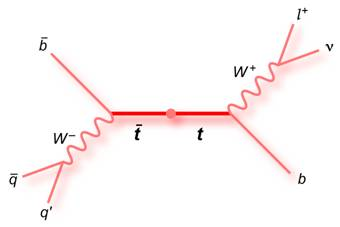
\includegraphics[width=0.5\textwidth]{TopAnalysis/figures/TopFeynmann.jpg}
  \caption[Semileptonic $t\bar{t}$ decay]{Semileptonic $t\bar{t}$ decay}
  \label{fig:topfeynmann}
\end{figure}

Here we give details of an analysis proposed for measuring the top quark forward-backward asymmetry, A$_{FB}^t$, at CLIC during the 1.4 TeV stage. 

As already described in Chapter \ref{theory}, A$_{FB}^t$ is sensitive to the electroweak form factors of the ttX(X=Z,$\gamma$) vertex. By measuring A$_{FB}^t$ and the $t\bar{t}$ cross section at multiple energies and with different beam polarizations it is possible to extract values for the electroweak form factors and use these as a probe for testing the \ac{SM} and searching for \ac{BSM} physics. This measurement is well motivated by the existing result for the b quark forward-backward asymmetry as measured at \ac{LEP}, which currently provides the largest deviation from the \ac{SM} within electroweak fits. Due to the limited energy at \ac{LEP} (which is still the highest energy e$^+$e$^-$ collider to have existed,) no analagous measurement of the asymmetry for tops has ever been performed at a lepton collider. 

\begin{table}
  \centering
  \begin{tabular}{l |c}
    \toprule
    Decay Mode     & Branching Fraction (\%) \\
    \midrule
    Fully Hadronic & 45.3  \\
    $tt\rightarrow WbWb\rightarrow qqbqqb$ & \\
    \midrule
    Semileptonic & 43.8 \\
    $tt\rightarrow WbWb\rightarrow qqbl\nu b$ &  \\
    \midrule
    Fully Leptonic & 10.6 \\
    $tt\rightarrow WbWb\rightarrow l\nu bl\nu b$ &  \\
    \midrule
    $tt\rightarrow Other$ & 0.4 \\
    \bottomrule
  \end{tabular}
  \caption{Top Pair Decay Modes}
  \label{table:topdecaymodes}
\end{table}

A$_{FB}$ is defined as:

\begin{equation}
A_{FB}^t=\frac{N_F-N_B}{N_F+N_B}
\end{equation}
Where N$_{F}$ and N$_{B}$ are the number of top quarks produced in the forward and backward directions which are defined to be the hemispheres corresponding to an angle of less than and greater than 90$^0$ relative to the direction of motion of the electrons initial momentum respectively.

As tops decay almost exclusively to a W and b (99.8\% of decays) they are typically described in terms of the resulting decay modes of the Ws. The dominant decay modes are described in \reftab{table:topdecaymodes}. Here we will look at measuring $A_{FB}^{t}$ using the semileptonic $t\bar{t}$ decay channel (see \reffig{fig:topfeynmann}) in which one of the W's decays to a lepton and neutrino and the other W decays to a a pair of quarks. This decay mode is ideal as the lepton from the leptonically decaying top provides the ability to charge tag the top while the fully hadronic decay allows an accurate measurement of the production angle of the top, both of which are necessary for measuring $A_{FB}^{t}$ to high precision. Due to the sensitivity of $A_{FB}^{t}$ to polarization states, the measurment will be done for two different electron beam polarizations, -80\% and +80\%, assuming an even split of luminosity between the two configurations. The dominant signal and background processed examined by this analysis, as well as their cross sections and production ID numbers for each polarization are shown in \reftabs{table:topsamplesnegpol} and \ref{table:topsamplespospol}. All samples are simulated using the CLIC\_ILD\_CDR detector model. This is a variation of the ILD detector model developed for use at the ILC. The samples also include an overly of $\gamma\gamma\rightarrow$ hadron events from beamstrahlung based on a 30~ns window around the generated physics events. The dominant backgrounds are expected to be from alternative $t\bar{t}$ decays (fully hadronic decay modes and semileptonic decays containing taus) and from single top events (see \reffig{fig:singletop}) which will have very simliar topologies due to the fact they can both contain a hadronically decaying top.

\begin{figure}
  \centering
  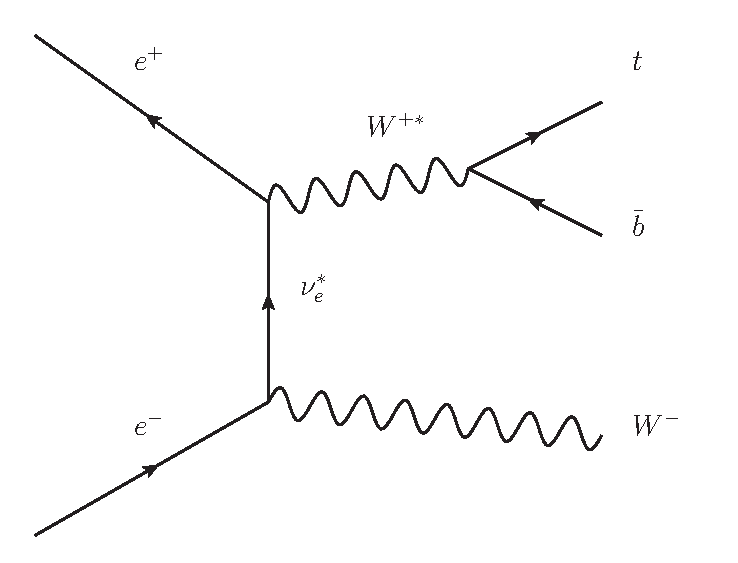
\includegraphics[width=0.5\textwidth]{TopAnalysis/figures/SingleTop}
  \caption[Dominant single top production mode]{Dominant single top production mode capable of mimicking the signal process}
  \label{fig:singletop}
\end{figure}

\begin{table}
  \centering
  \begin{tabular}{l | r | r |r}
    \toprule
    Process     & Cross Section(fb) & Production ID & Events Used (10$^{-3}$) \\
    \midrule
    $e^+e^-\rightarrow qqqql\nu$ & 142.3 & 6589,6592,6634,6637 & 3860 \\
    \midrule
    $e^+e^-\rightarrow qqqqqq$ & 116.4 & 6595, 6598, 6601, 6604,  & 310 \\
     &  & 6610, 6607, 6613, 6616,  &  \\
     &  &  6619, 6622  &  \\
    \midrule
    $e^+e^-\rightarrow qql\nu l\nu$ & 44.1 & 6586, 6625, 6628, 6631 & 100 \\
    \midrule
    $e^+e^-\rightarrow qqqq$ & 2304.0 & 8254 & 1,590 \\
    \midrule
    $e^+e^-\rightarrow qql\nu$ & 6975.0 & 7477 & 3,520 \\
    \midrule
    $e^+e^-\rightarrow qqll$ & 2681.0 & 8244 & 1,190 \\
    \midrule
    $e^+e^-\rightarrow qq\nu\nu$ & 1395.0 & 8271 & 1,120 \\
    \midrule
    $e^+e^-\rightarrow qq$ & 4843.0 & 8283 & 2,400 \\
    \bottomrule
  \end{tabular}
  \caption{Samples used in the -80\% electron beam polarization study}
  \label{table:topsamplesnegpol}
\end{table}

\begin{table}
  \centering
  \begin{tabular}{l | r | r |r}
    \toprule
    Process     & Cross Section(fb) & Production ID & Events Used (10$^{-3}$) \\
    \midrule
    $e^+e^-\rightarrow qqqql\nu$ & 53.5 & 6646, 6697, 6691, 6694 & 160 \\
    \midrule
    $e^+e^-\rightarrow qqqqqq$ & 44.9 & 6652, 6655, 6658, 6661, & 198 \\
     &  & 6664, 6667, 6670, 6673, &  \\
     &  & 6676, 6679 &  \\
    \midrule
    $e^+e^-\rightarrow qql\nu l\nu$ & 15.3  & 6643, 6682, 6685, 6688 & 15.3 \\
    \midrule
    $e^+e^-\rightarrow qqqq$ & 347 & 8257 & 500 \\
    \midrule
    $e^+e^-\rightarrow qql\nu$ & 1640 & 7480 & 1,000 \\
    \midrule
    $e^+e^-\rightarrow qqll$ & 2530 & 8241 & 1,000 \\
    \midrule
    $e^+e^-\rightarrow qq\nu\nu$ & 180 & 8274 & 200 \\
    \midrule
    $e^+e^-\rightarrow qq$ & 3170 & 8286 & 1,500 \\
    \bottomrule
  \end{tabular}
  \caption{Samples used in the +80\% electron beam polarization study}
  \label{table:topsamplespospol}
\end{table}


\section{Event Reconstruction}
Reconstruction of the signal events is performed using ILCSOFT v01-17-10 and consists of three main stages. The first stage is to identify isolated leptons arising from the leptonically decaying top. These leptons are then removed and the remaining PFOs are resolved into two large radius ``fat jets''. These two fat jets must then be associated with either the b jet produced by the leptonically decaying top or to the combination of three jets arrising from the hadronically decaying top. A kinematic fitter is then used to reconstruct the neutrino and any \ac{ISR}/\ac{BS} photons present in the event.

\subsection{Lepton Finding}

Lepton finding is the first stage of reconstruction performed in each event. Due to the fact the measurement of $A_{FB}^{t}$ is entirely reliant on using the lepton charge to distinguish between top and antitop decays, it is essential that a high efficiency and purity are achieved and that there is no angular dependence on the performance. For this analysis lepton finding is done in two steps. Firstly, lepton candidates with energy $>$ 10~GeV are identified using the particle ID provided by the Pandora Particle Flow Algorithm \cite{Thomson200925}. Only muons and electrons are examined due to the fact tau leptons require different reconstruction techniques to identify and are typically reconstructed with significantly lower efficiency. This first stage removes $>$ 90\% of fake candidates with negligible impact on efficiency. The second stage of lepton selection is to examine how isolated each of the candidates are. This is evaluated by resolving all PFOs in the event into five jets, then for each lepton candidate measuring the energy of the candidate relative to the jet it was been associated with. For this process the inclusive ee kt algorithm was chosen for the jet finding to ensure that all lepton candidates are always placed within a jet. The lepton candidate found to have the highest ratio of $E_{Candidate}/E_{Jet}$ is then declared to be the isolated lepton arrising from the letonically decaying top. In the event that no lepton is selected by the first step, the restrictions on the particle ID and energy are relaxed and the lepton is selected purely based on which PFO is the most isolated according to step two. This method ensures that there is always exactly one lepton selected per event. The net efficiency with which this method selects a candidate with the correct charge is found to be 93\% for electrons and 96\% for muons.

As well as understanding the net efficiency for finding leptons it is also important to examine the angular dependence of the efficiency to ensure there is no bias that could effect the measurement of $A_{FB}^{t}$. \reffig{fig:netefficiency} shows how the efficiency varies with angle. The efficiency is seen to rapidly decline for $|Cos\theta| > 0.9$ due to detector acceptances. A decrease in efficiency is also seen for electrons at angles corresponding to the transition point between the ECAL barrel and endcaps. This effect is not seen for muons as they are also reconstructed using the muon detectors placed at a larger radius. Overall the efficiency is seen to be consistently worse for electrons than muons. This is to be expected as muons produce easily recognisable signatures in the detector due to the fact they typically penetrate through the tracker, ECAL, HCAL and muon sytems whereas electrons only leave deposits in the tracker and ECAL. In the case that tracks are lost during reconstruction or are wrongly associated to other PFOs it is then possible for photons to wrongly be labelled as electrons and vice versa leading to a higher fake rate for electrons.

\begin{figure}
  \centering
  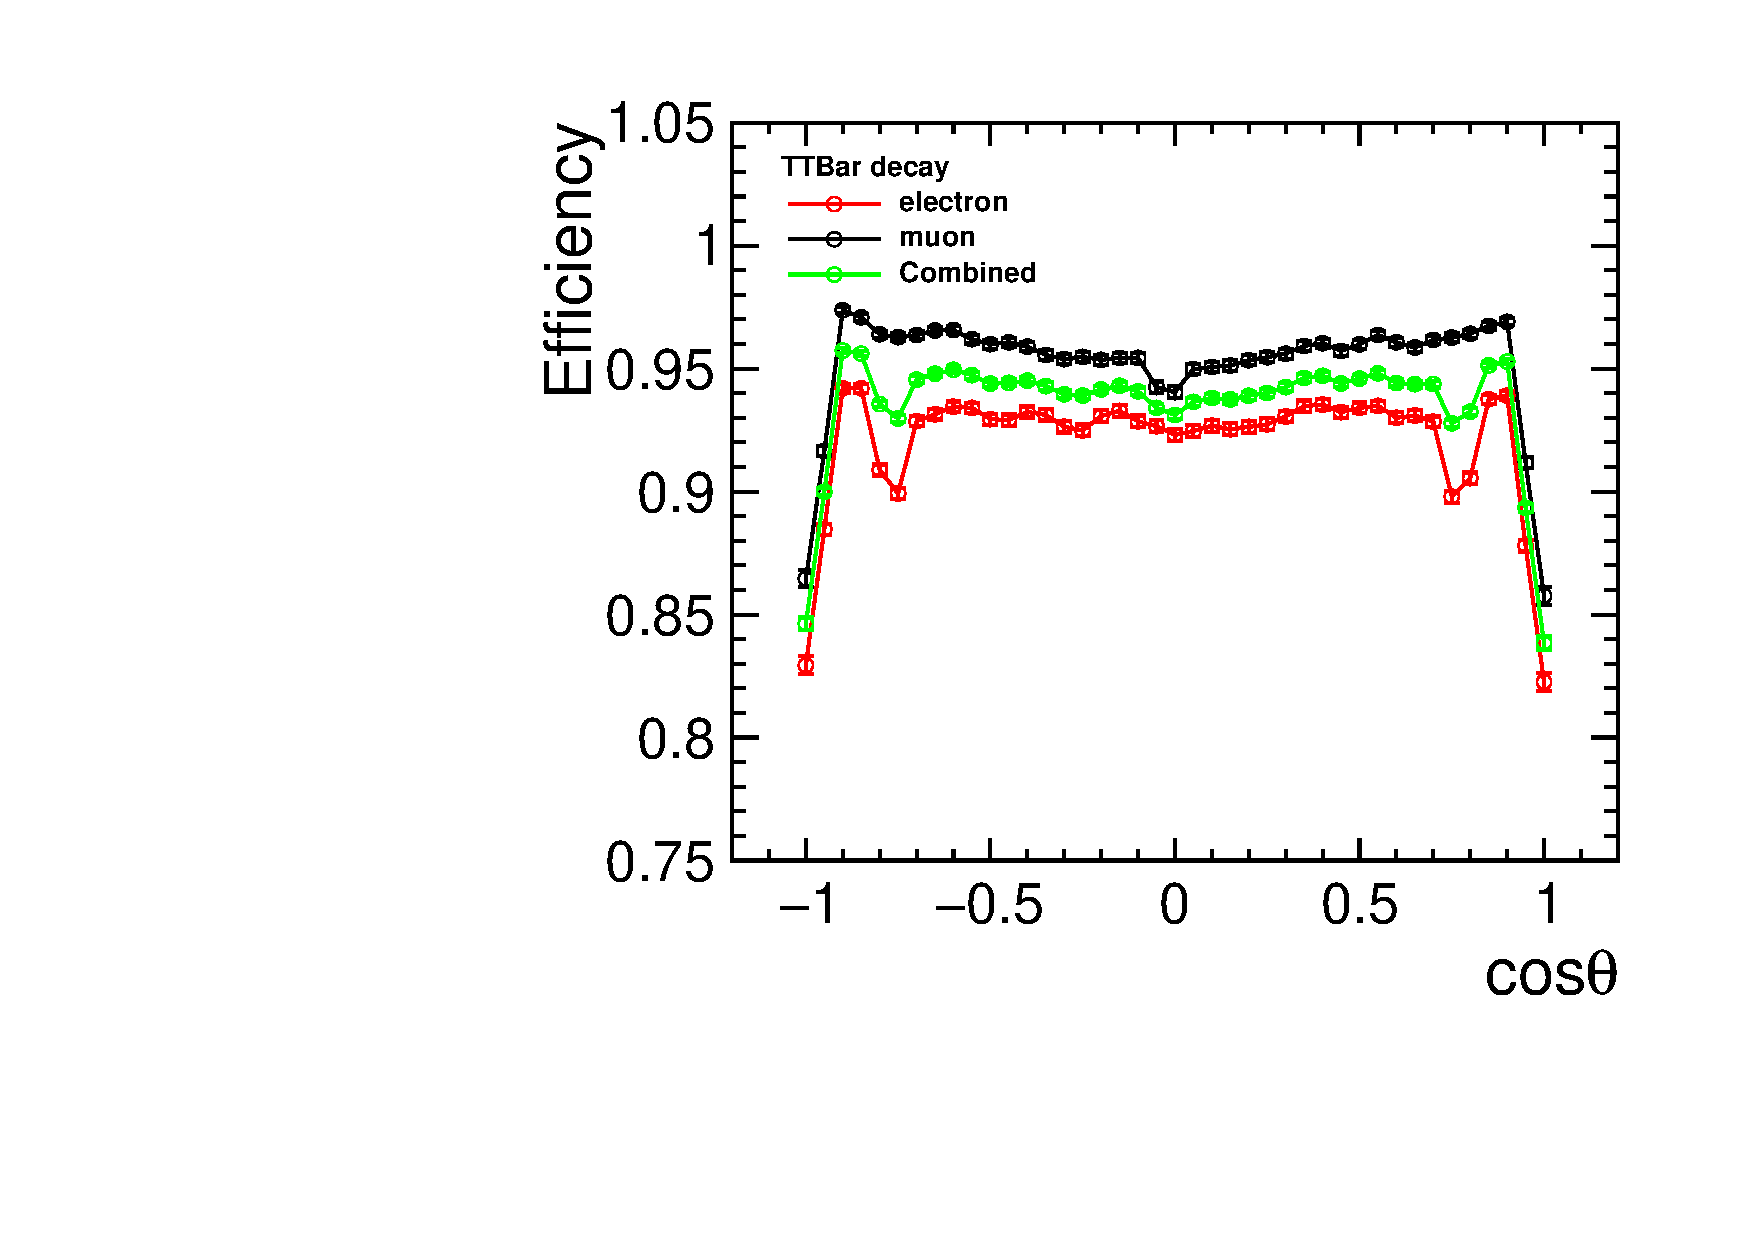
\includegraphics[width=0.6\textwidth]{TopAnalysis/figures/NetEfficiencys.pdf}
  \caption[Charge Tagging Efficiency]{Efficiency for identifying leptons with the correct charge as a function of angle}
  \label{fig:netefficiency}
\end{figure}

As well as checking the angular dependence of the charge tagging efficiency it is also key to examine the charge dependence of the lepton finding to make sure there is no preference for identifying particles over antiparticles. The angular dependence of the charge tagging efficiency for particles vs antiparticles is shown in \reffig{fig:chargeEfficiencies}. An asymmetry in the performance is observed in both electrons and muons.

\begin{figure}
  \centering
  \begin{subfigure}{.5\textwidth}
    \centering
    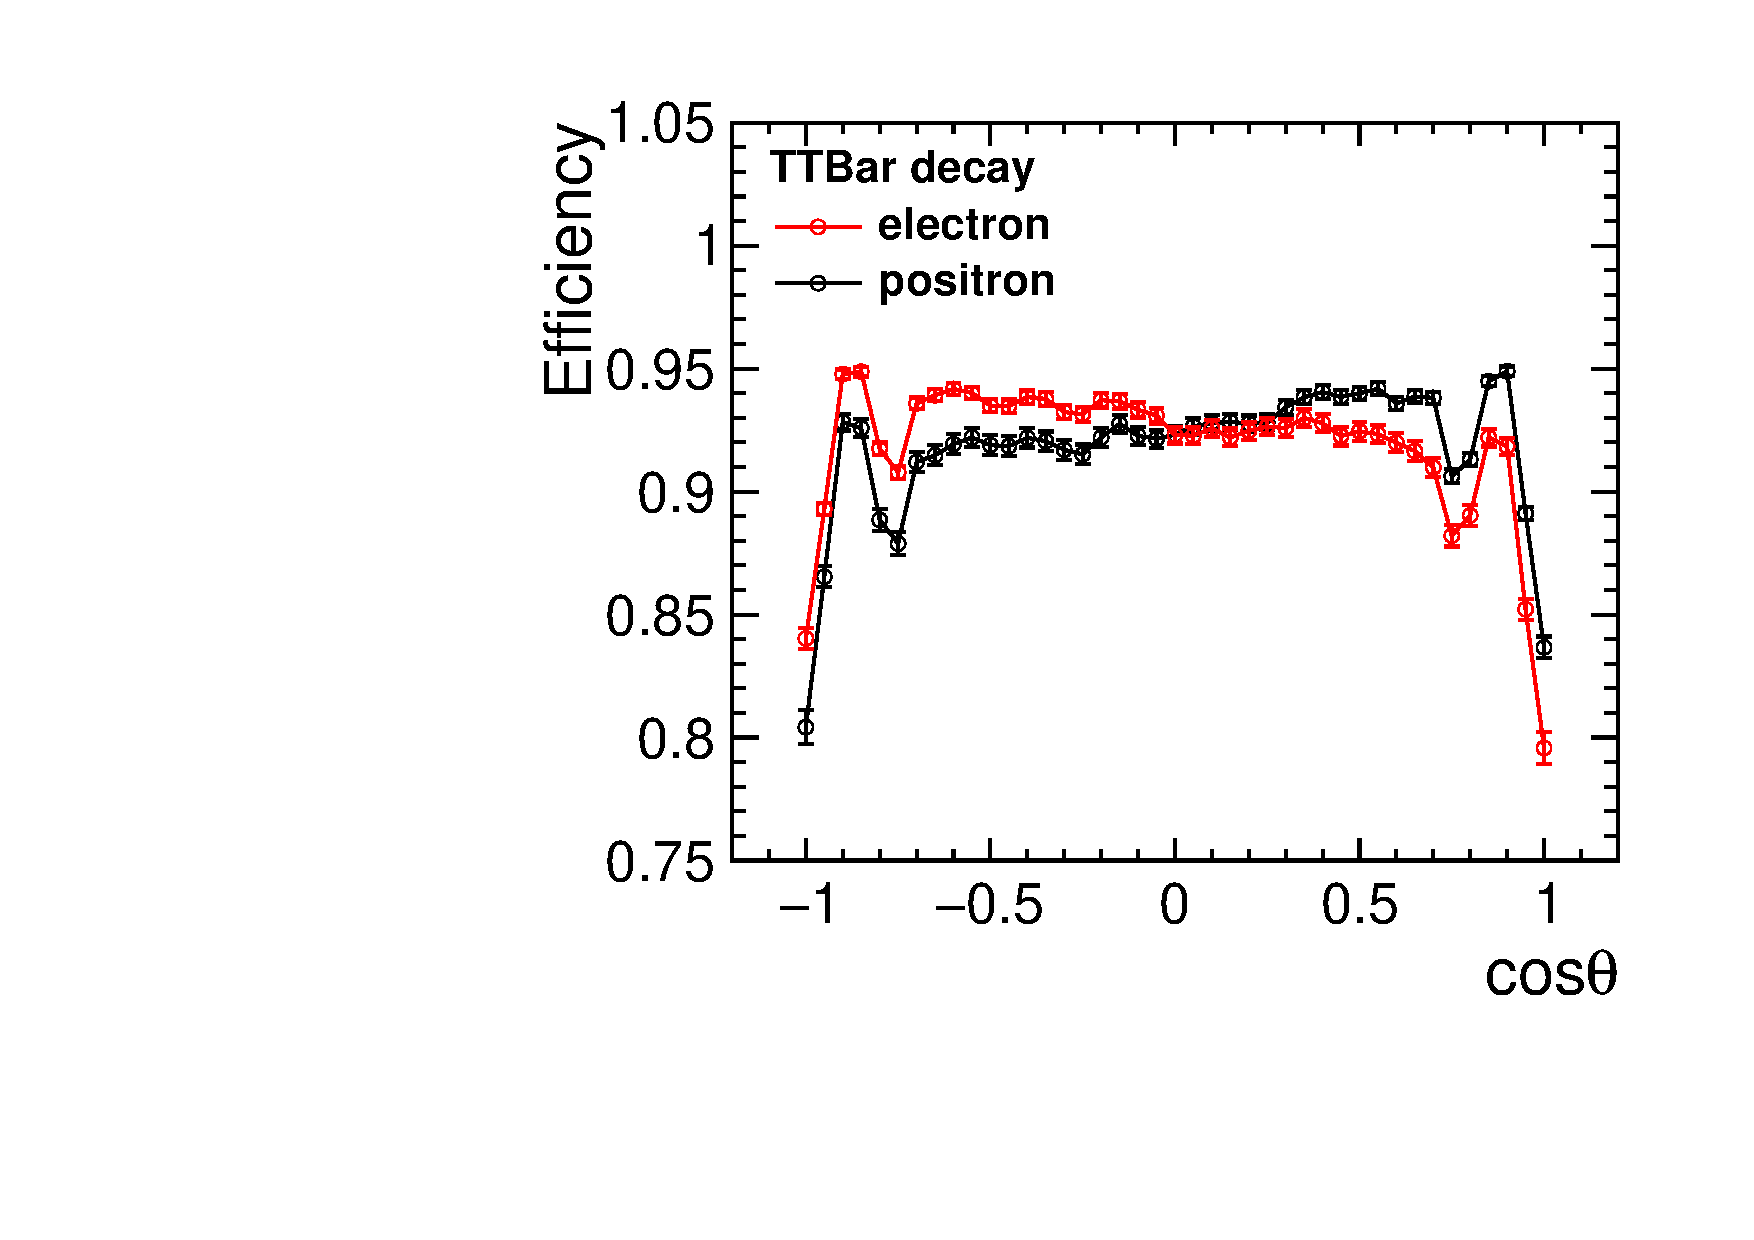
\includegraphics[width=0.9\textwidth]{TopAnalysis/figures/ElectronEfficiencys.pdf}
    \caption[Charge Tagging Efficiency]{Electrons}
    \label{fig:electronefficiency}
  \end{subfigure}%
  \begin{subfigure}{.5\textwidth}
    \centering
    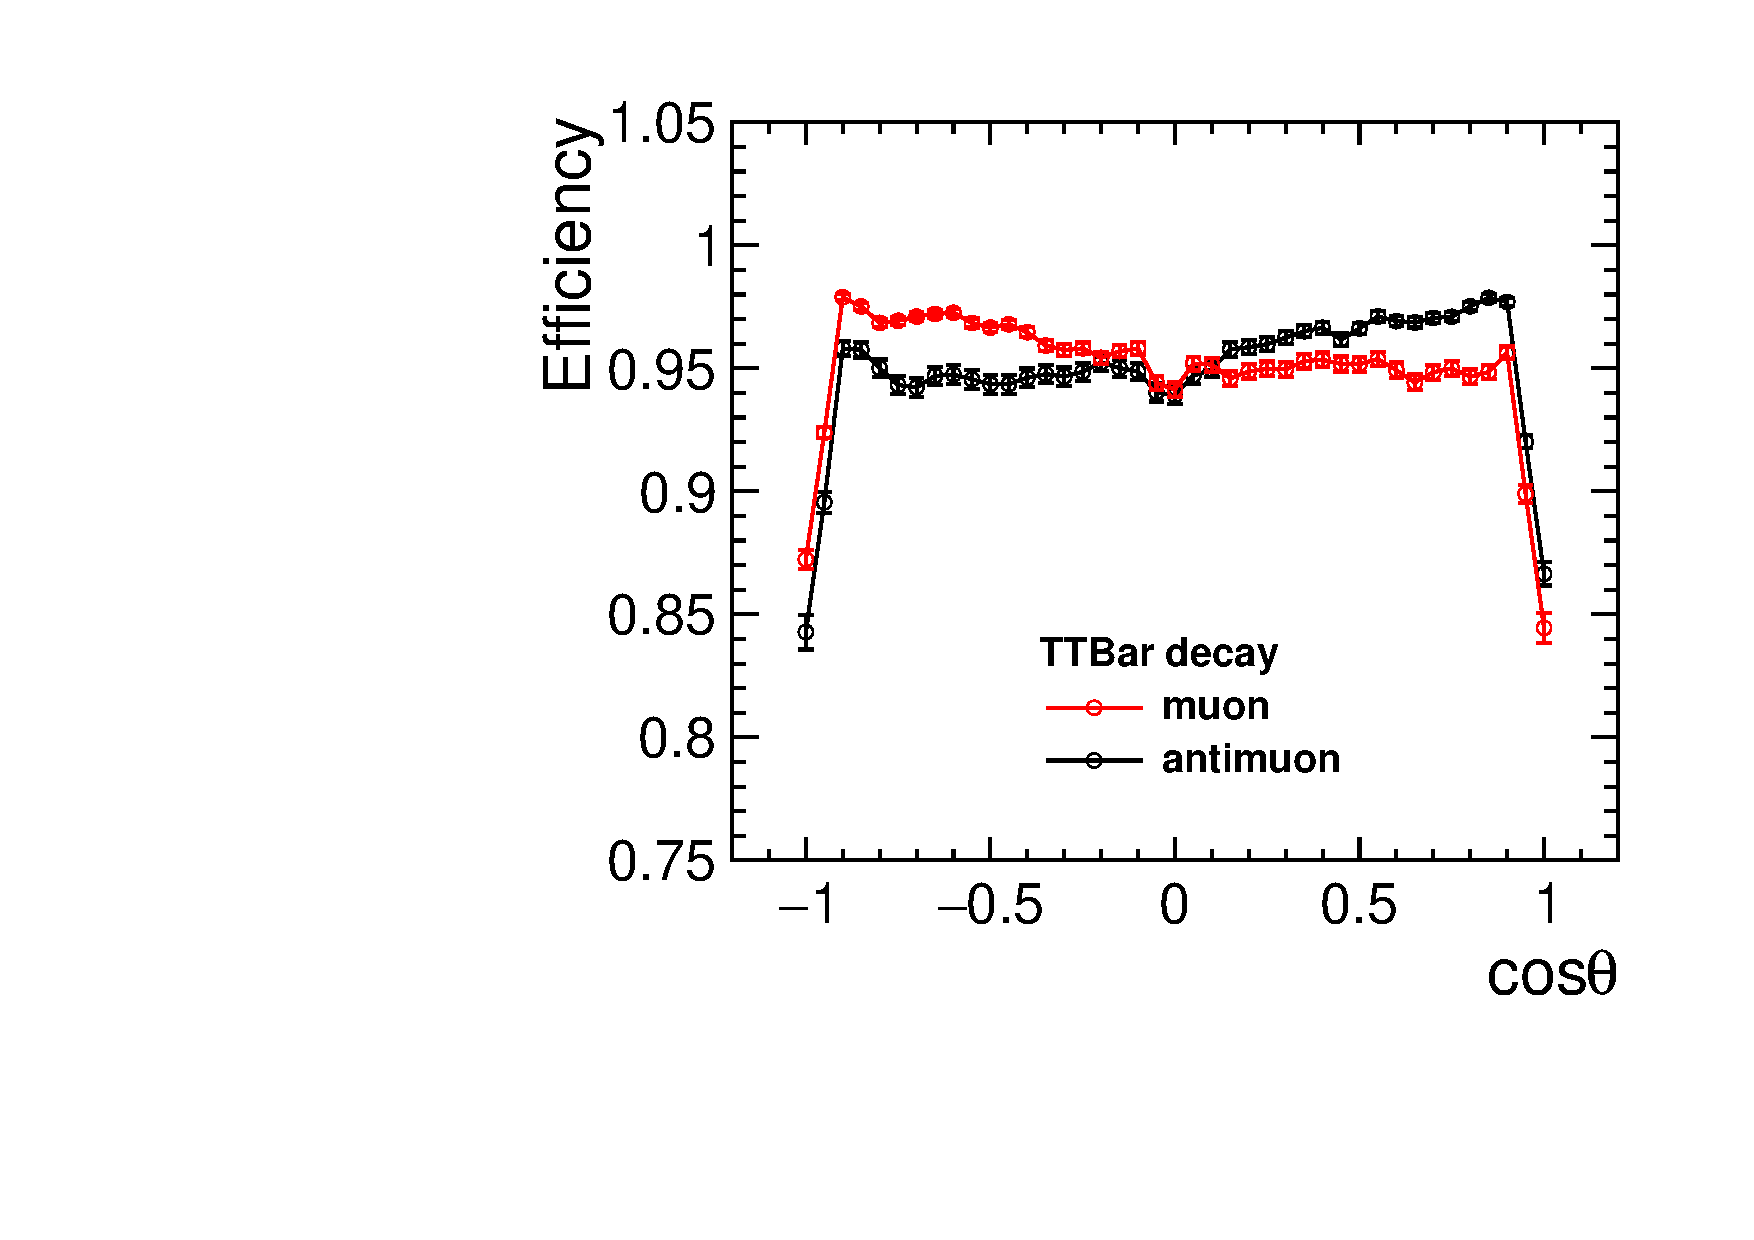
\includegraphics[width=0.9\textwidth]{TopAnalysis/figures/MuonEfficiencys.pdf}
    \caption[Charge Tagging Efficiency]{Muons}
    \label{fig:muonefficiency}
  \end{subfigure}
  \caption{Angular dependence of lepton finding for particles vs antiparticles}
  \label{fig:chargeEfficiencies}
\end{figure}

It arises from the underlying asymmetry in the production of particles vs antiparticles due to forward-backward asymmetries. The forward backward asymmetry means that tops are preferencialy produced in one direction while antitops are produced more often in othe opposite direction, however due to charge conservation this also means that the W bosons and leptons are produced asymmetrically too. Because the collisions are taking place well above the top pair production threshold, the W bosons will gain a large boost forcing them to travel in the same direction as the inital top. The polarization of the W also means that the lepton will also be preferencially produced along the same diection as the W and can only be produced in the opposite direction with a lower energy. Overall this means that leptons are produced with higher energy in one direction and lower energy in the opposite direction while for antileptons this directional dependence is reversed. The effect is shown in \reffig{fig:efficiency2d} where it is seen that positrons are produced with higher energy in the forward direction($cos\theta>0$) than the backward direction. It is known that the efficiency for reconstructing leptons at CLIC increases with energy and so the fact the energy and angle at which leptons are produced are correlated results in the asymmetric angular efficiency for correctly reconstructing the lepton. Further evidence for this theory is shown in \reffig{fig:higgsleptons} and \ref{fig:effienciesWithCuts} which show that the asymmetry disappears when either the production mode for the leptons is symmetric or when low energy leptons are not included.

\begin{figure}
  \centering
  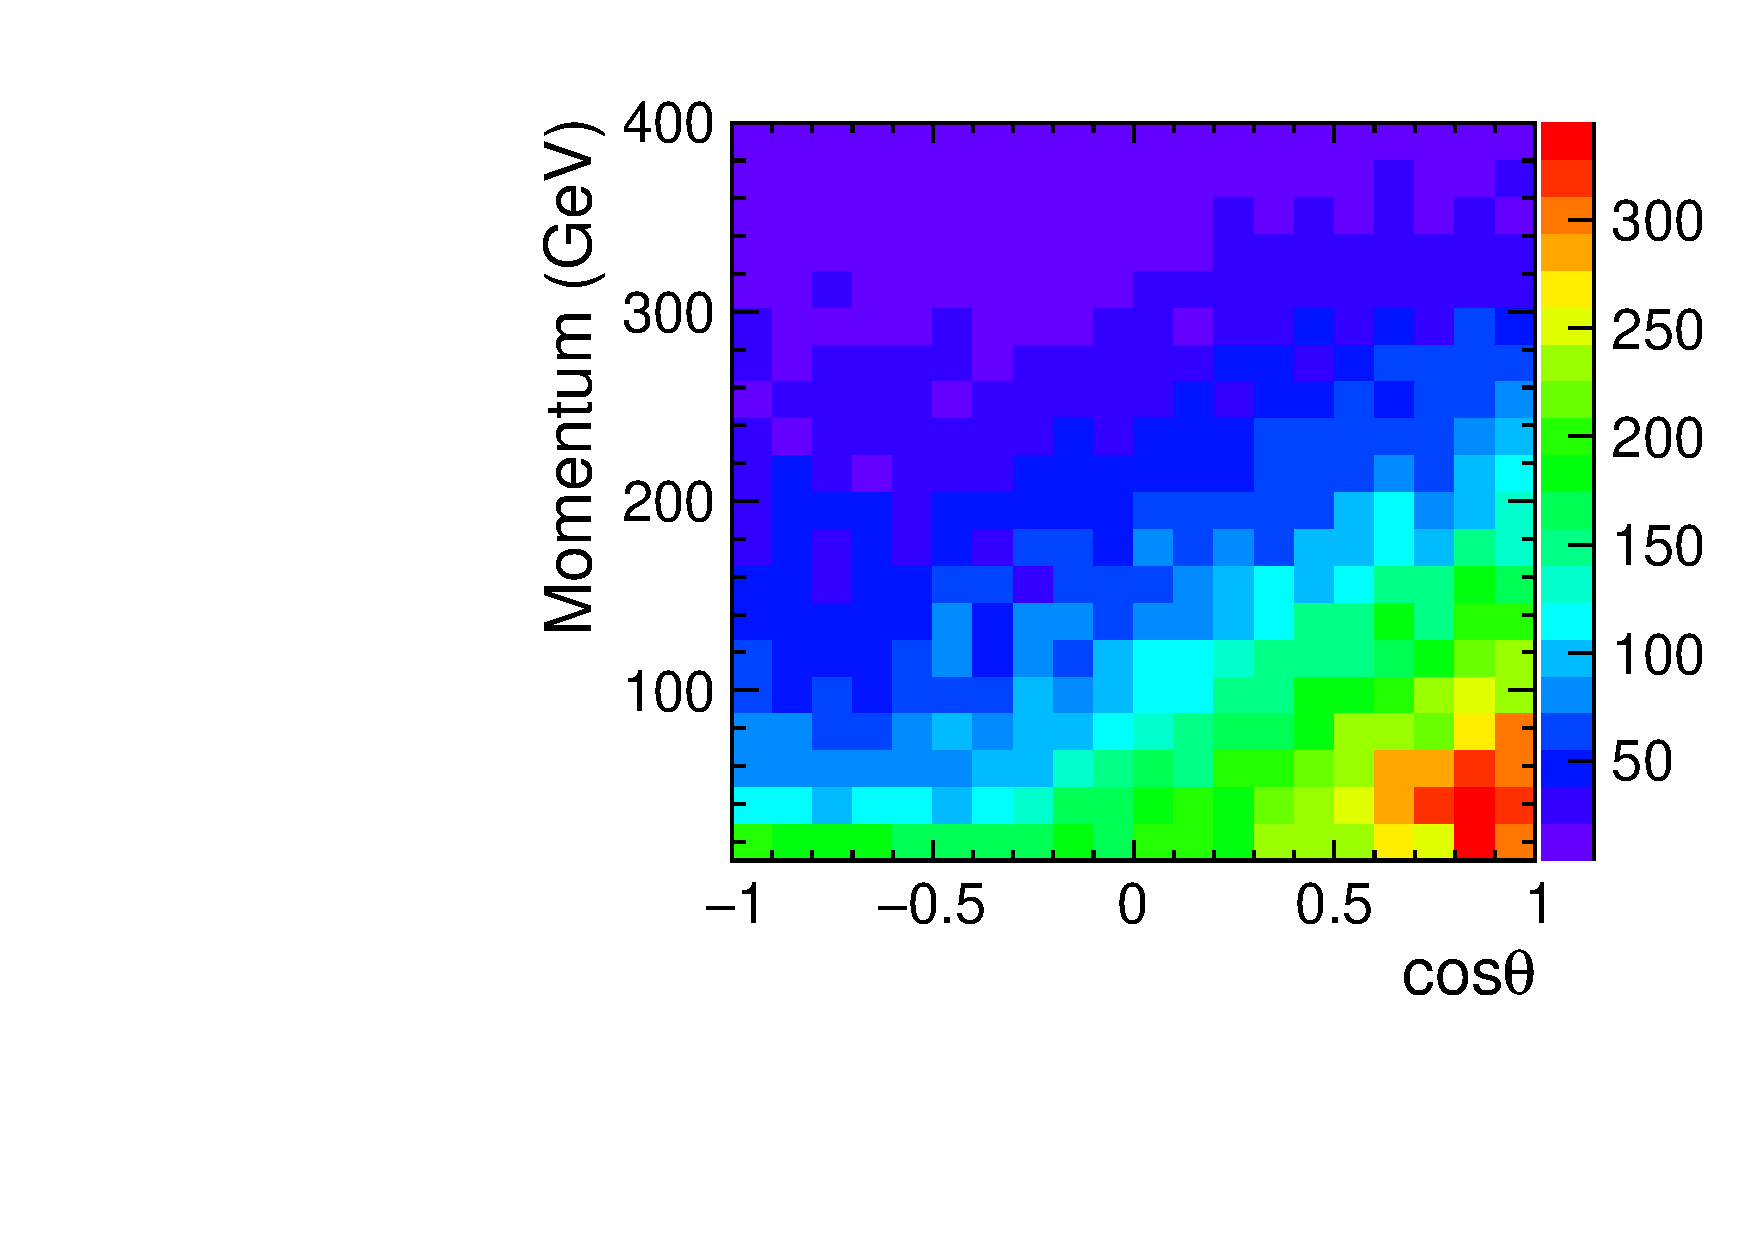
\includegraphics[width=0.6\textwidth]{TopAnalysis/figures/MomentumVsTheta.pdf}
  \caption[Lepton Momentum Vs Angle]{Correlation between lepton momentum and angle for positrons only}
  \label{fig:efficiency2d}
\end{figure}

\begin{figure}
  \centering
  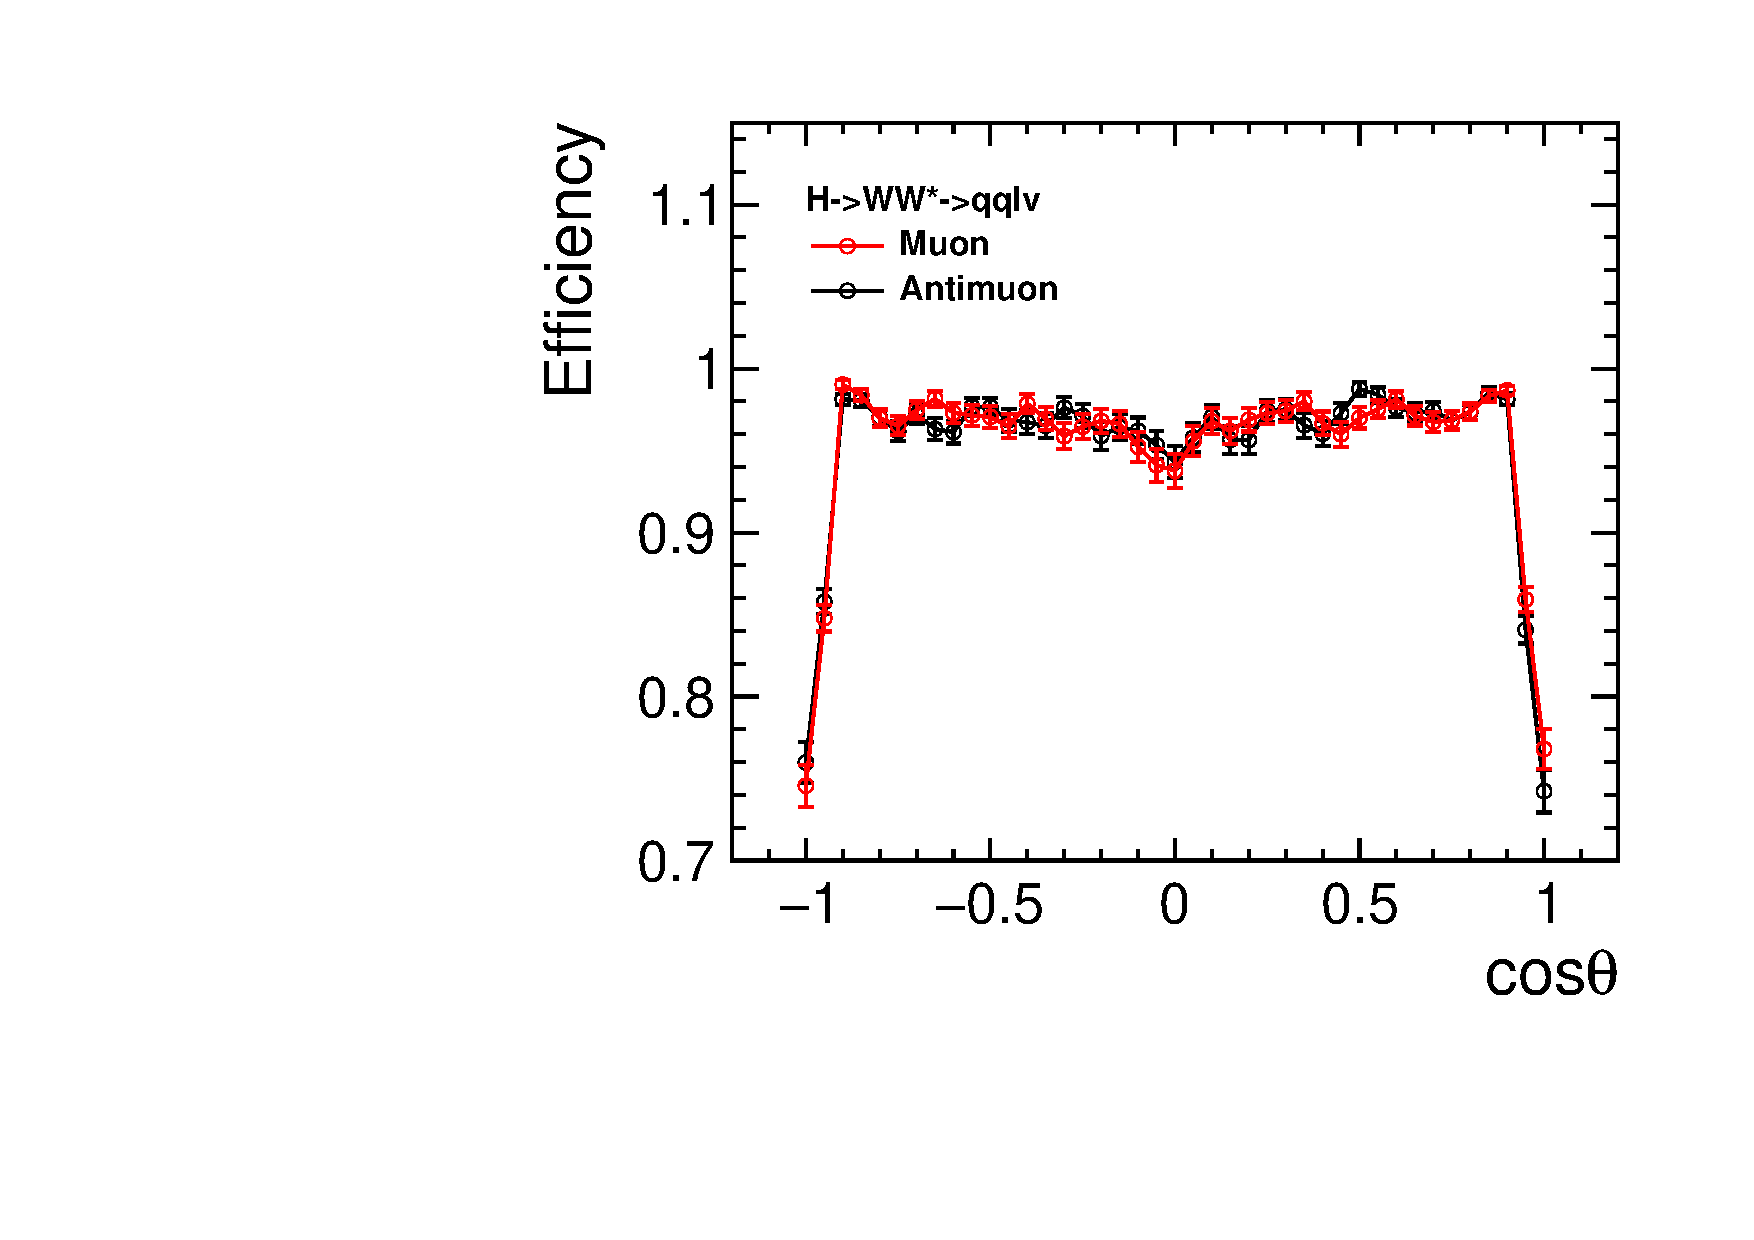
\includegraphics[width=0.6\textwidth]{TopAnalysis/figures/MuonEfficiency_Higgs.pdf}
  \caption[Lepton efficiency for $ee\rightarrow H\nu\nu,H \rightarrow WW\rightarrow qql\nu$ ]{Charge tagging efficiency for $ee\rightarrow H\nu\nu,H \rightarrow WW\rightarrow qql\nu$. The efficiency is seen to be symmetric for particles and antiparticles when they are produced with the same initial angular distribution.}
  \label{fig:higgsleptons}
\end{figure}

\begin{figure}
  \centering
  \begin{subfigure}{.5\textwidth}
    \centering
    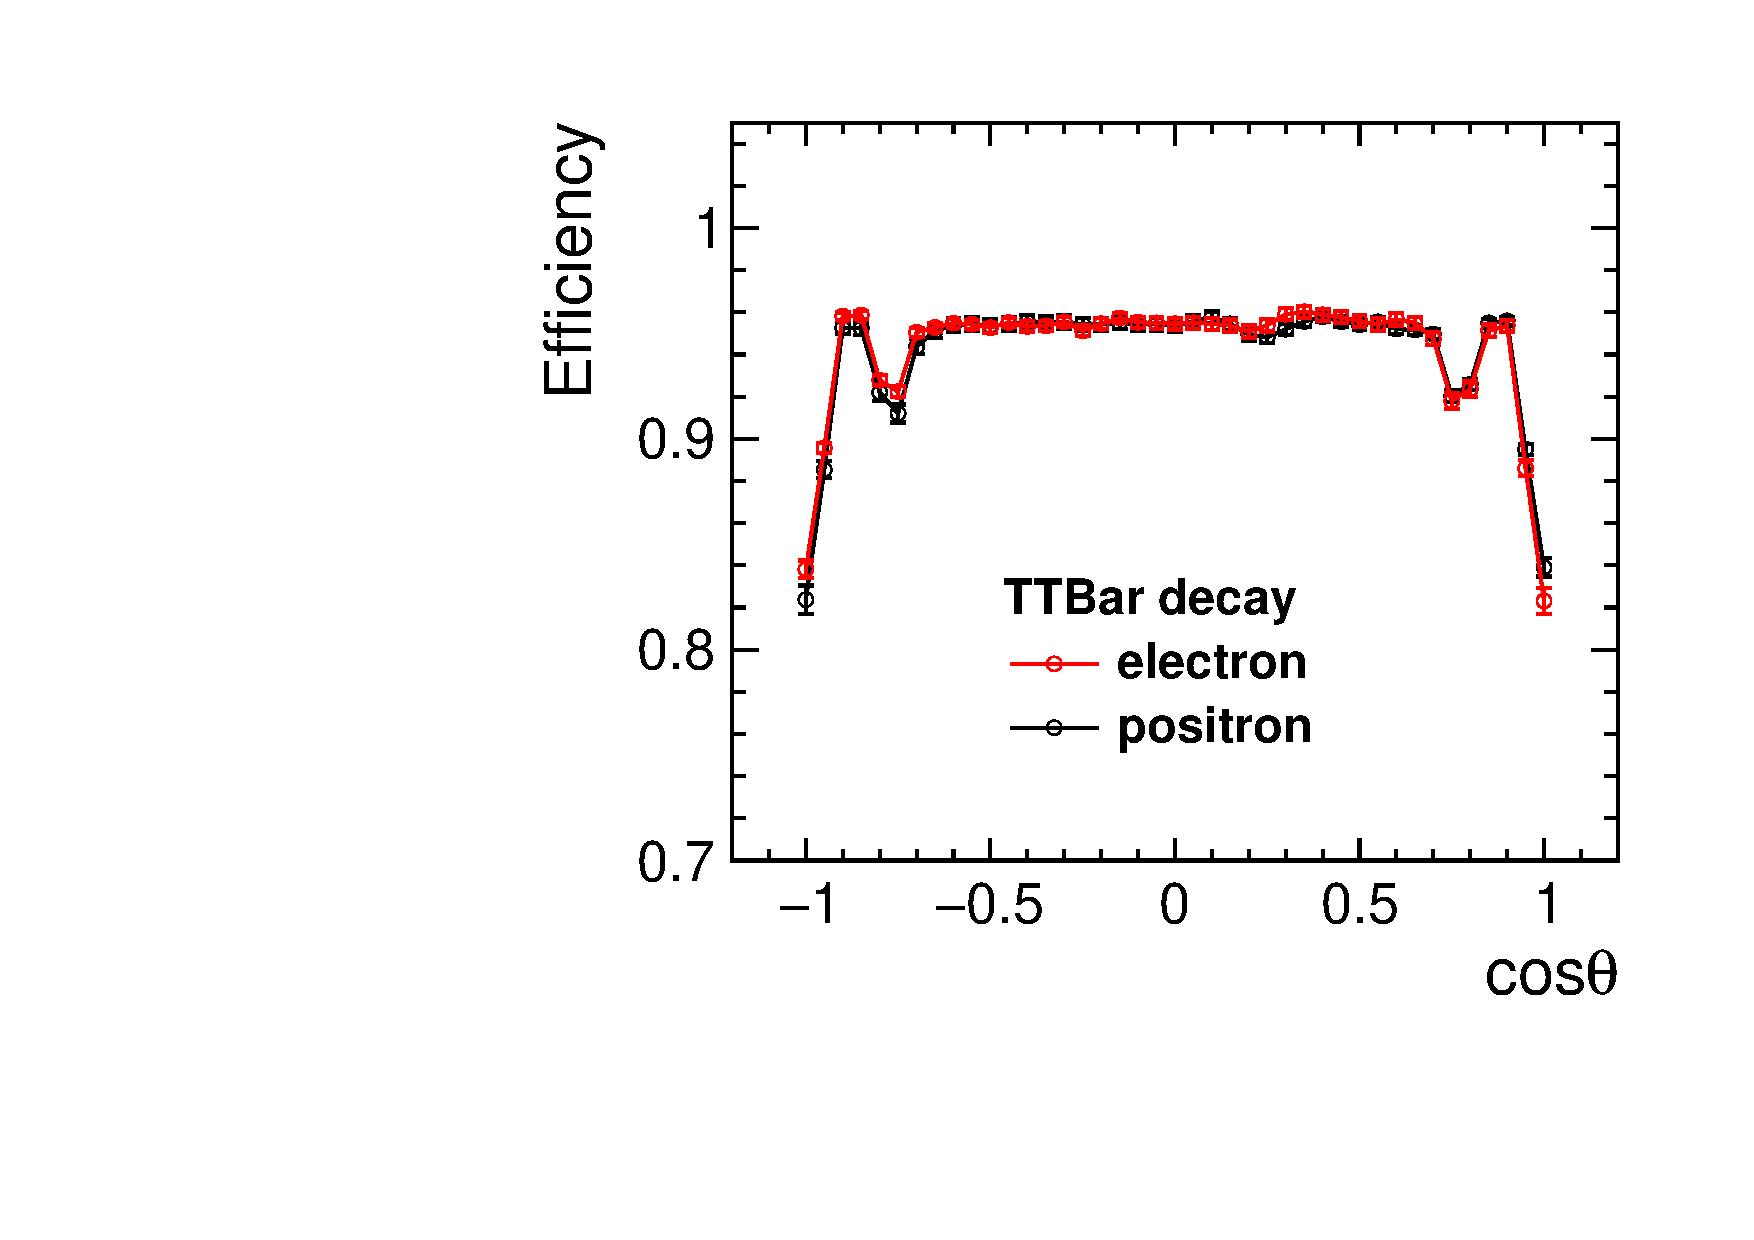
\includegraphics[width=0.9\textwidth]{TopAnalysis/figures/ElectronEfficiencys_20GeVMCCut.pdf}
    \caption[Charge Tagging Efficiency]{Electrons}
  \end{subfigure}%
  \begin{subfigure}{.5\textwidth}
    \centering
    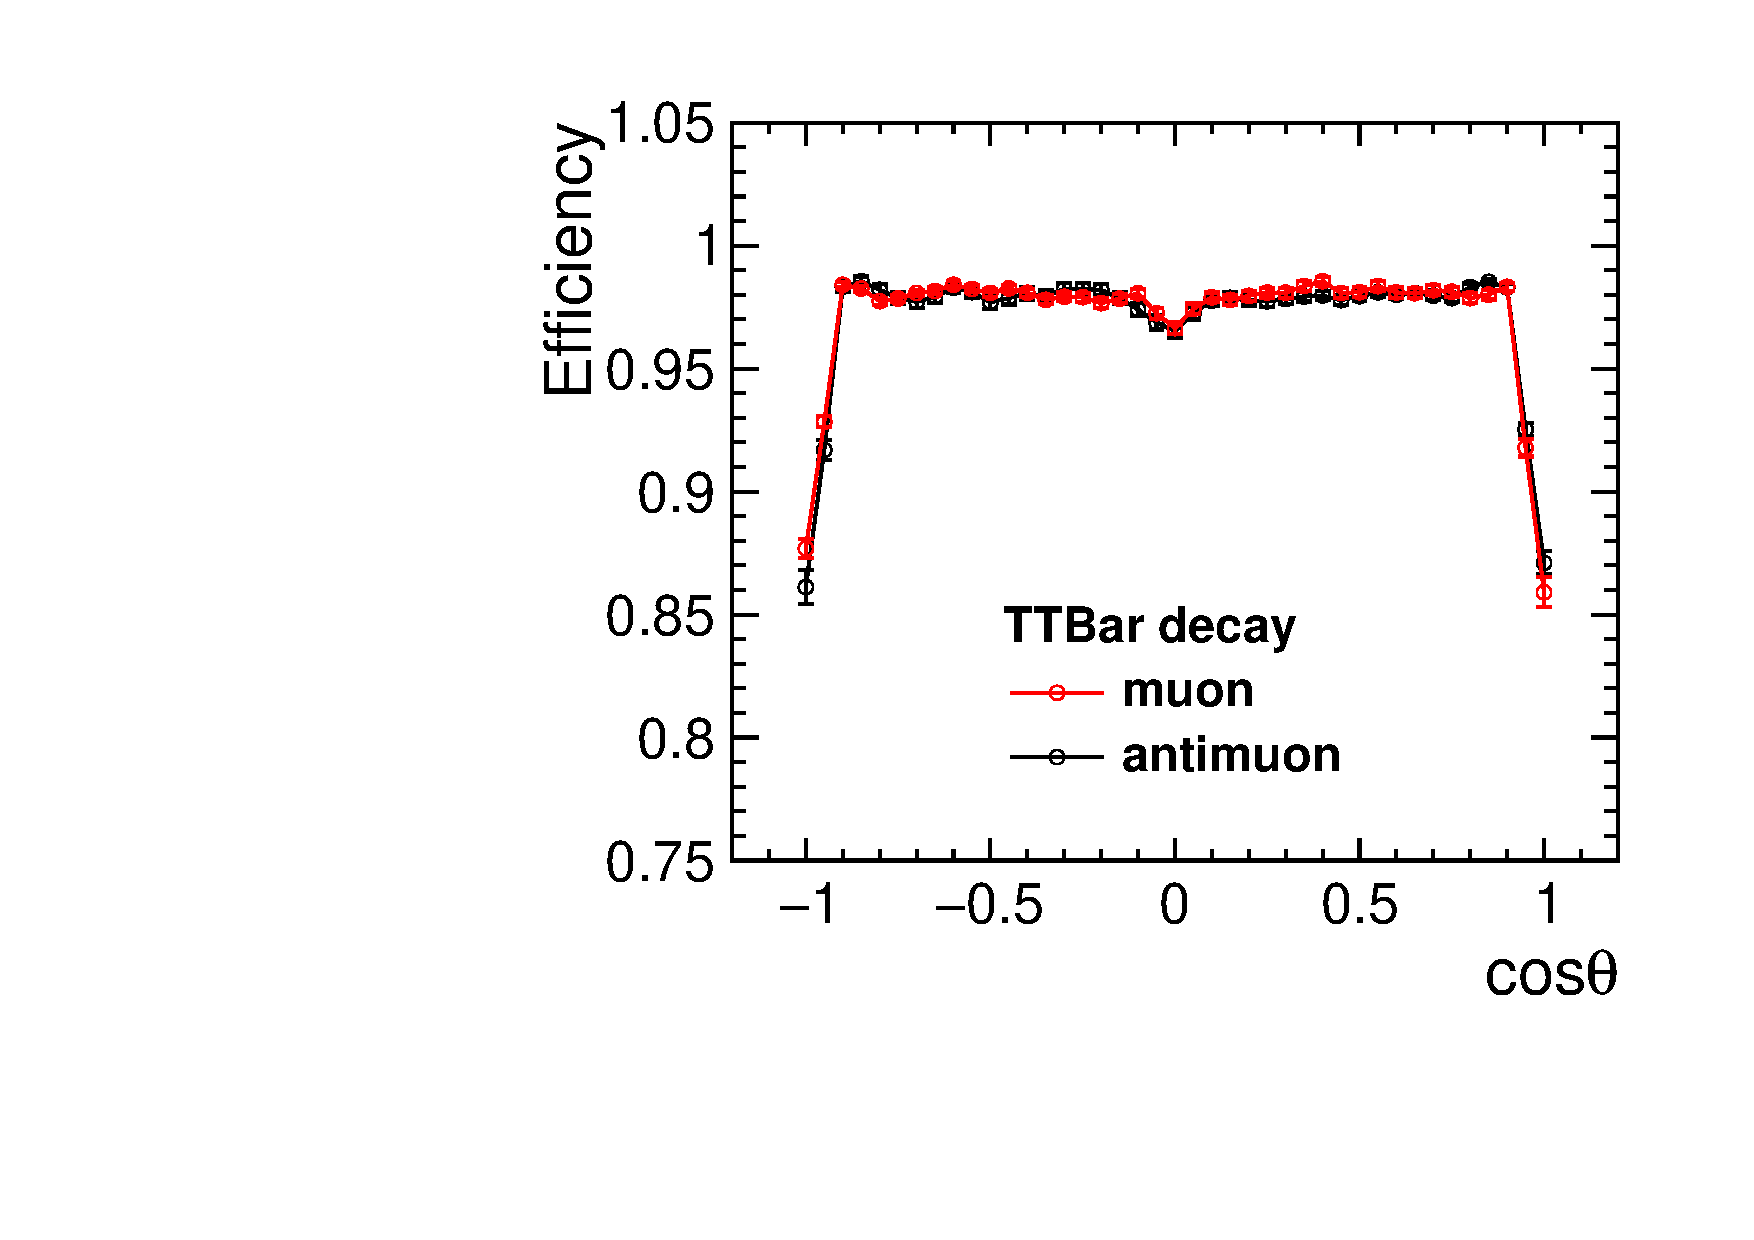
\includegraphics[width=0.9\textwidth]{TopAnalysis/figures/MuonEfficiencys_20GeVMCCut.pdf}
    \caption[Charge Tagging Efficiency]{Muons}
  \end{subfigure}
  \caption[Charge Tagging Efficiency After 20GeV Lepton Momentum Cut]{Charge tagging efficiency after 20~GeV lepton momentum cut. The efficiency is seen to be symmetric for leptons with momentum $>$ 20~GeV}
  \label{fig:effienciesWithCuts}
\end{figure}


\subsection{Fat Jet Finding}

\begin{figure}
  \centering
  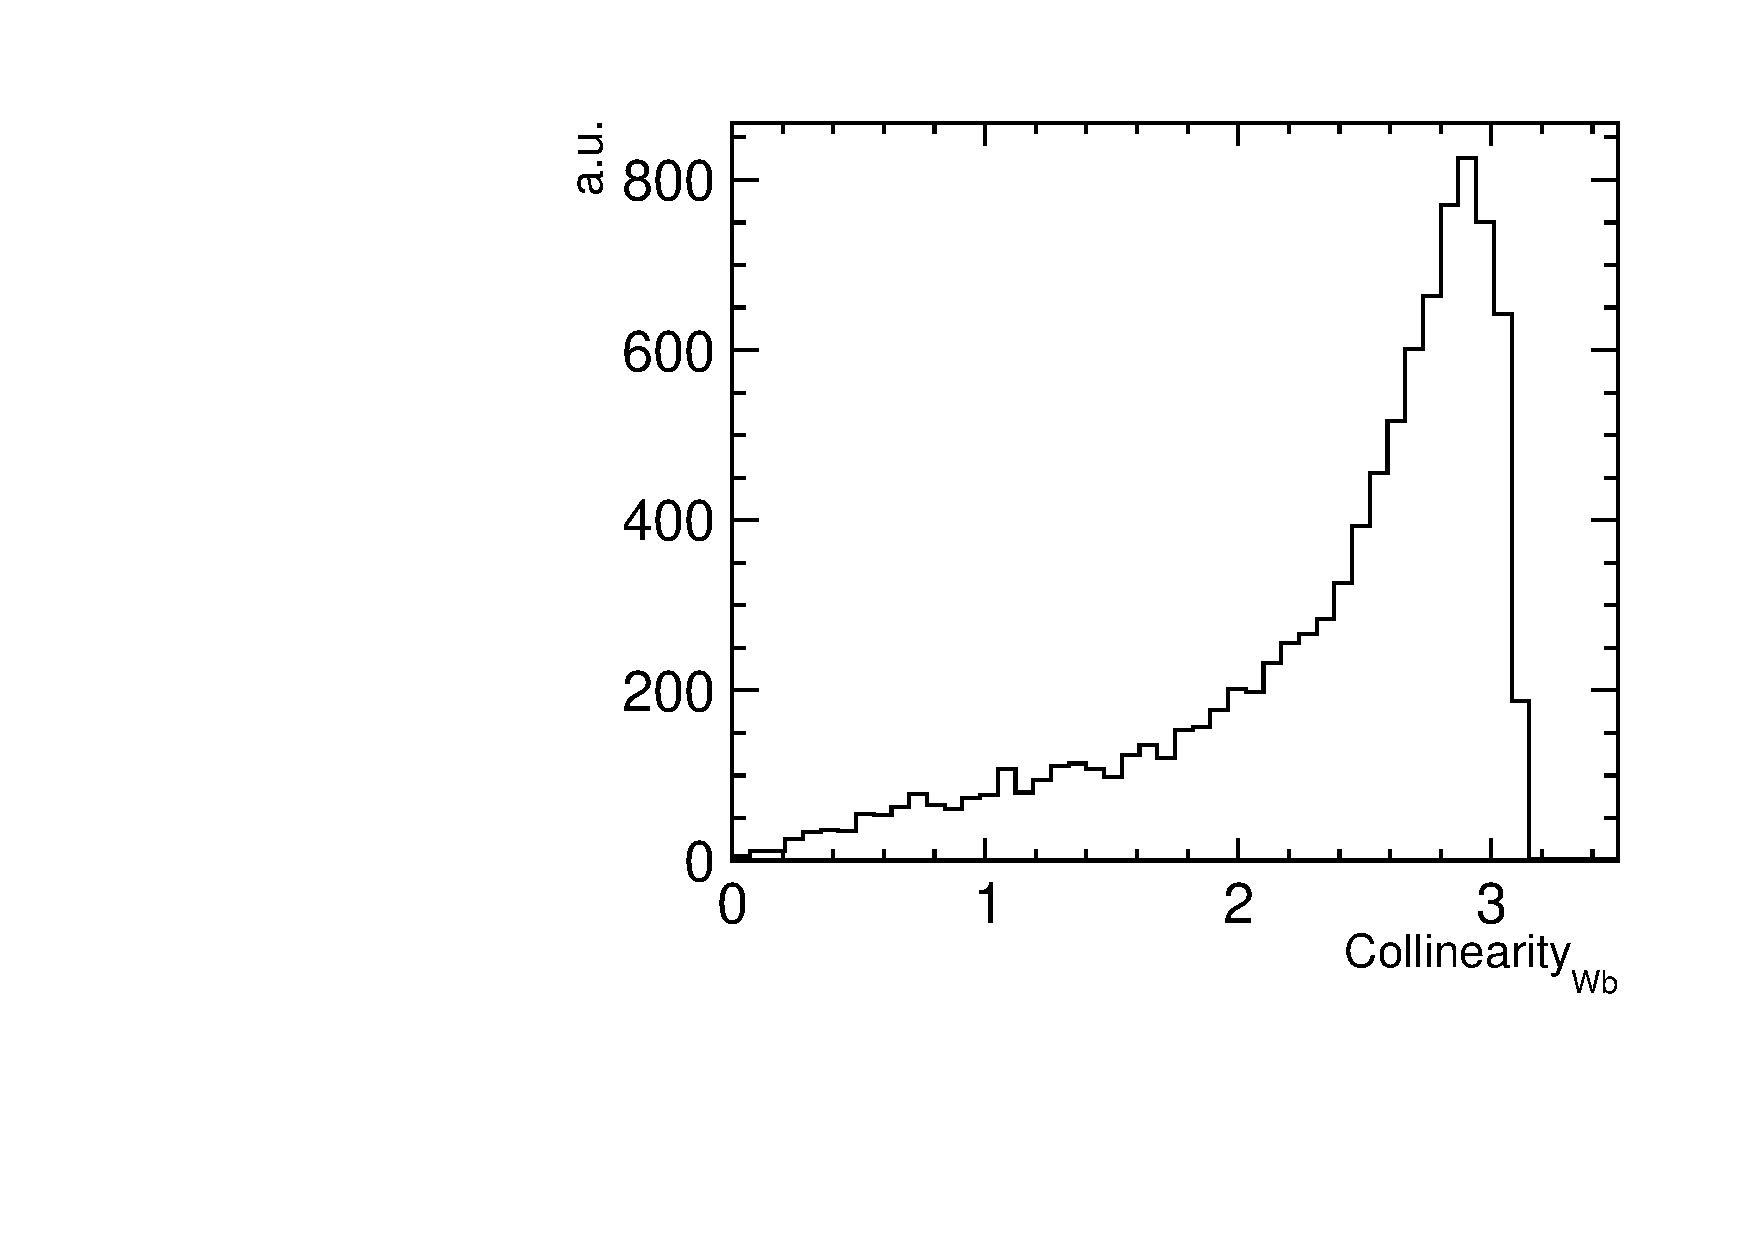
\includegraphics[width=0.6\textwidth]{TopAnalysis/figures/WBCollinearity.pdf}
  \caption[Separation between W and b jet from top decay]{Separation between W and b jets from top decay. The pair are typically too collimated to allow the b-jet and the pair of jets from the W decay to be successfully resolved into three distinct jets}
  \label{fig:Collimated}
\end{figure}

Jet reconstruction was performed using the FastJet package \cite{Cacciari:2011ma}. Due to the high energy of the collisions relative to the top mass, the tops produced are highly boosted and produce highly collimated decay products (see \reffig{fig:Collimated}.) This means it is typically not possible to resolve the decay products from the hadronically decaying top into three jets corresponding to the b-jet and light quark jets from the W decay. As a result an alternative approach to jet reconstruction is considered based on the concept of fat jets, an approach already being used at the LHC\cite{Miller:2011qg}. Fat jets are large radius jets and are used to cluster groups of jets that can't be accurately resolved individually into one larger jet. For the purpose of this anaylsis the events are clustered into fat jets which should correspond to the b-jet from the leptonically decaying top and to the whole set of decay products from the hadronically decaying top. The mass and substructure variables (see \refsec{Event Selection}) of these fat jets can then be used to distinguish genuine top events from backgrounds. Two jet algorithms were considered for reconstructing the fat jets- the longitudinally invaraint kt algorithm \cite{Cacciari:2008gp} and Valencia algorithm \cite{Boronat:2014hva}. The kt algorithm is already extensively used at hadron colliders while the Valencia algorithm is a newer algorithm designed for future lepton colliders that offers improved performance in handling beam backgrounds. A full description of the kt algorithm is already given in \refsec{higgsjetfinding} so here we will only describe the Valencia algorithm. Overall the Valenica algorithm is similar to the kt algorithm, however the key differences are that the inter-particle distance and beam distance are redefined as:

\begin{equation}
d_{ij}=min(E_i^{2\beta},E_j^{2\beta})(1-cos\theta_{ij})/R^2
\end{equation}
\begin{equation}
d_{iB}=p_T^{2\gamma}E^{2(\beta - \gamma)}
\end{equation}

Where R is the usual jet radius defined in the same way as for the kt algorithm and $\beta$ and $\gamma$ are additional parameters that can be used to tune how the algorithm behaves for particles approaching the beam line. \reffig{fig:valenciaPerformance} shows how the ratio $d_{ij}/d_{iB}$ develops for a pair of particles produced with fixed energy and angular separation as a function of their polar angle for multiple $\beta$ factors. One can see that a higher $\beta$ factor introduces a larger penalty for approaching the beam line leading to an decreased chance for the particles to be merged into a jet.

\begin{figure}
  \centering
  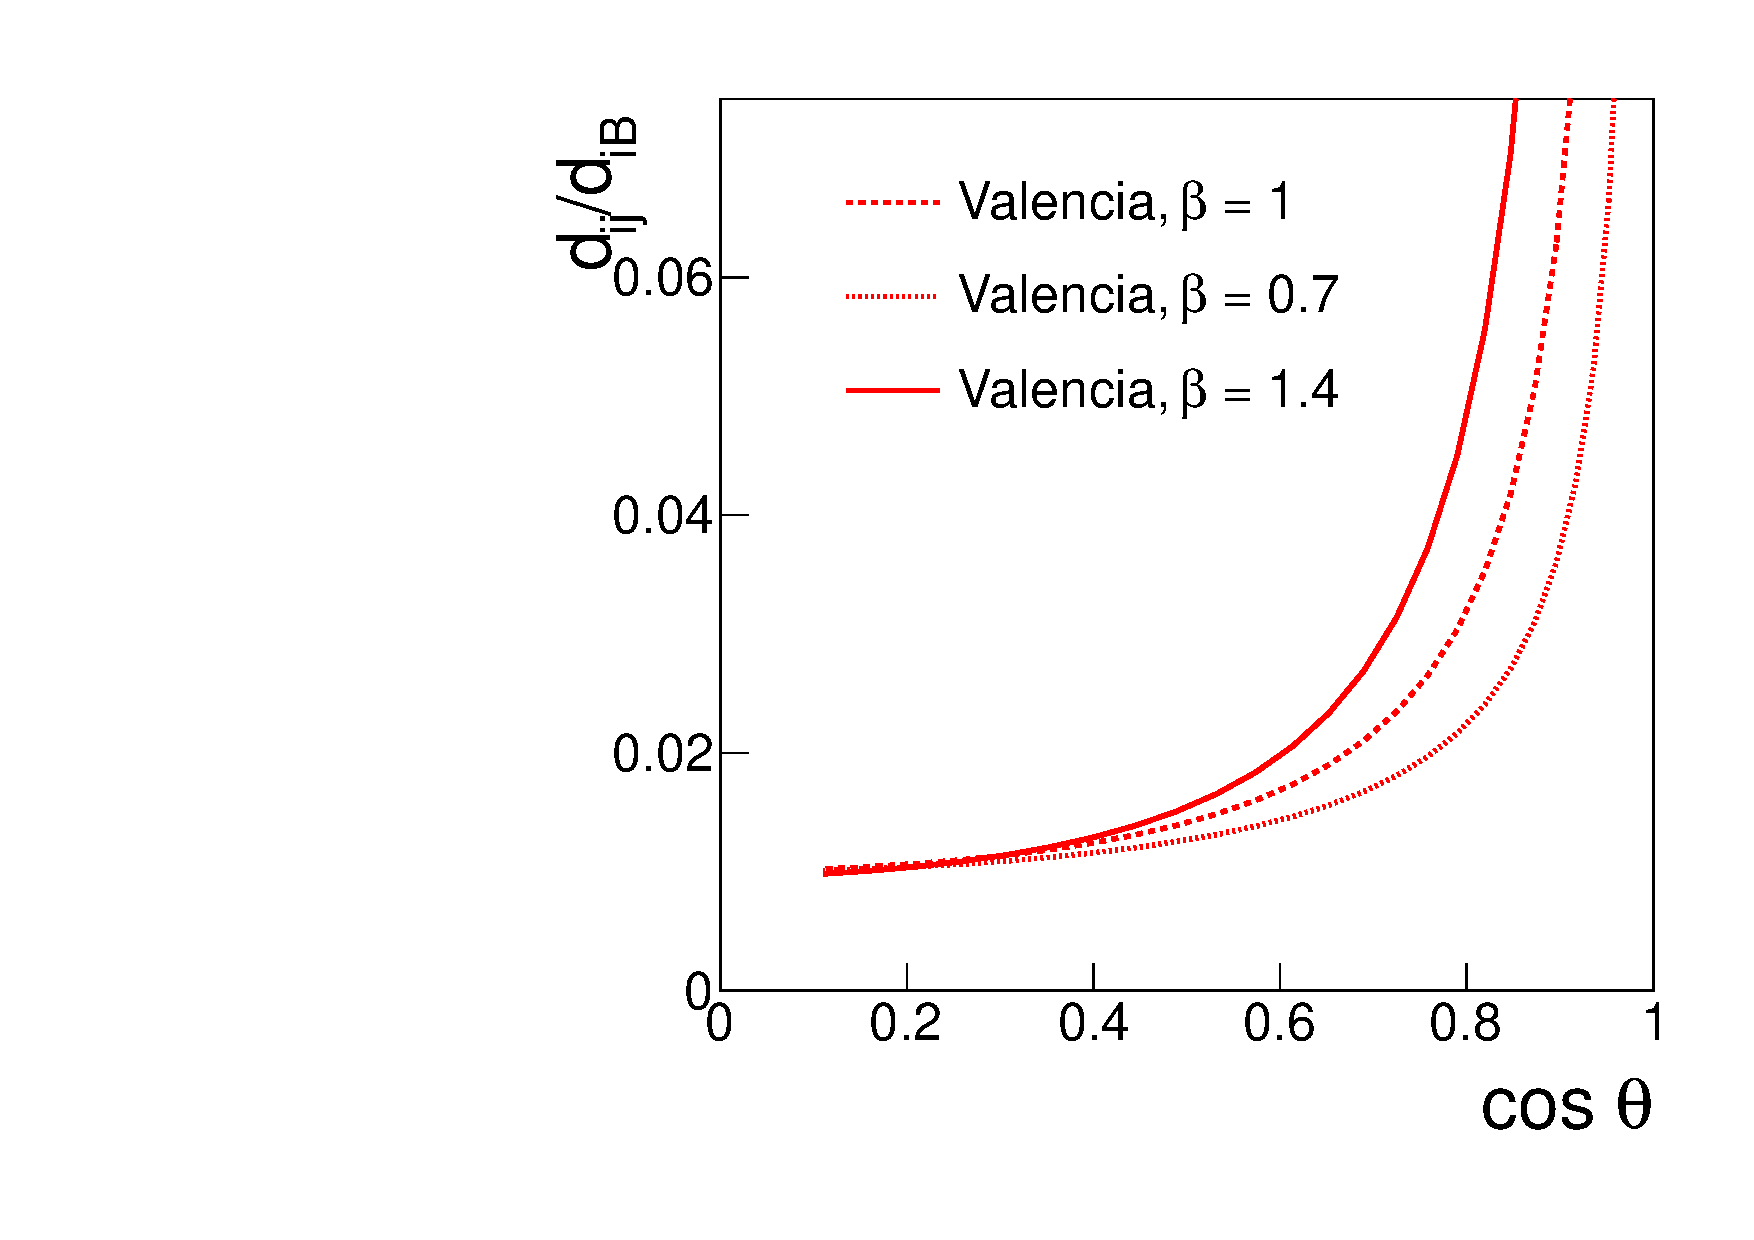
\includegraphics[width=0.6\textwidth]{TopAnalysis/figures/distance_ratio_vlc.pdf}
  \caption[Effect of the Valencia $\beta$ parameter]{Effect of the Valencia $\beta$ parameter on $d_{ij}/d_{iB}$ for a pair of particles produced at a fixed energy and angular separation as a function of their polar angle\cite{Boronat:2014hva}}
  \label{fig:valenciaPerformance}
\end{figure}

The performance of both algorithms is shown in figure \reffig{fig:jetfinding}. For both algorithms it is seen that at higher R the resolution on the top mass gets worse while for lower R sub-peaks start to appear in the mass distribution corresponding to partial reconstructions of the top (either a W Boson or single quark). The kt algorithm is seen to produce a consistently broader distribution in the top mass. Placing a cut on the collision energy of E $>$ 1.2~TeV reveals that these lower mass peaks only occur for lower collision energies where the tops will no longer be produced back to back and their decay products will be less collimated. As a result the fat jet finding can merge components from both the hadronic and leptonic tops into each jet. This analysis will be focusing on reconstructing the most boosted tops. As a result the Valencia algorithm is preferred due to it's better mass resolution. Performance for less boosted top decays might be improved by examining the performance of a more conventional jet analysis looking to resolve all four individual quarks whenever the fat jet finding produces jets outside the top mass window. This possibility is discussed later in \refsec{Quality Cuts}. Here the Valencia algorithm with R=1.5, $\beta$=1 and $\gamma$=1 is chosen as the optimal jet reconstrcution method to provide a balance between mass resolution and the frequency of partial reconstructions. 

\begin{figure}
  \centering
  \begin{subfigure}{.5\textwidth}
    \centering
    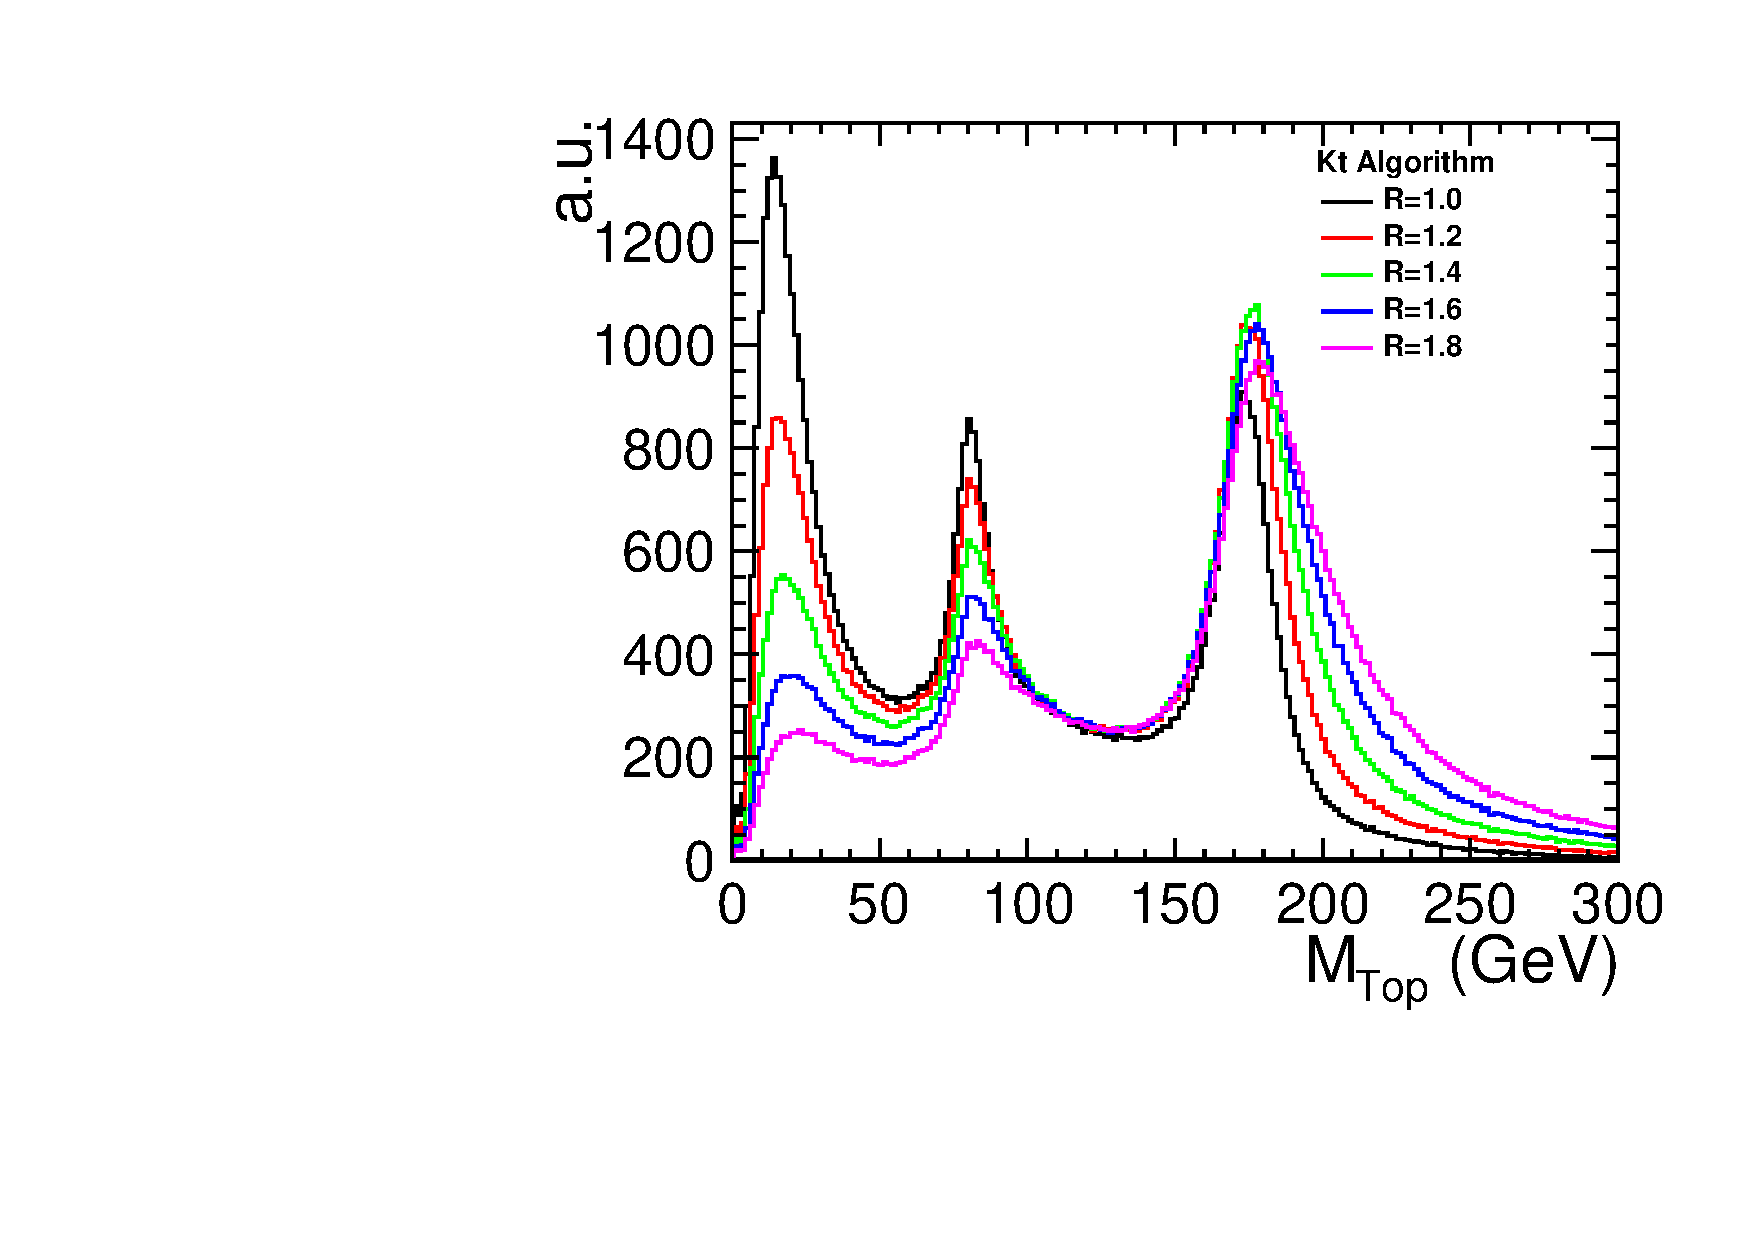
\includegraphics[width=1.0\textwidth]{TopAnalysis/figures/ComparisonKt.pdf}
    \caption[kt algorithm]{kt algorithm}
  \end{subfigure}%
  \begin{subfigure}{.5\textwidth}
    \centering    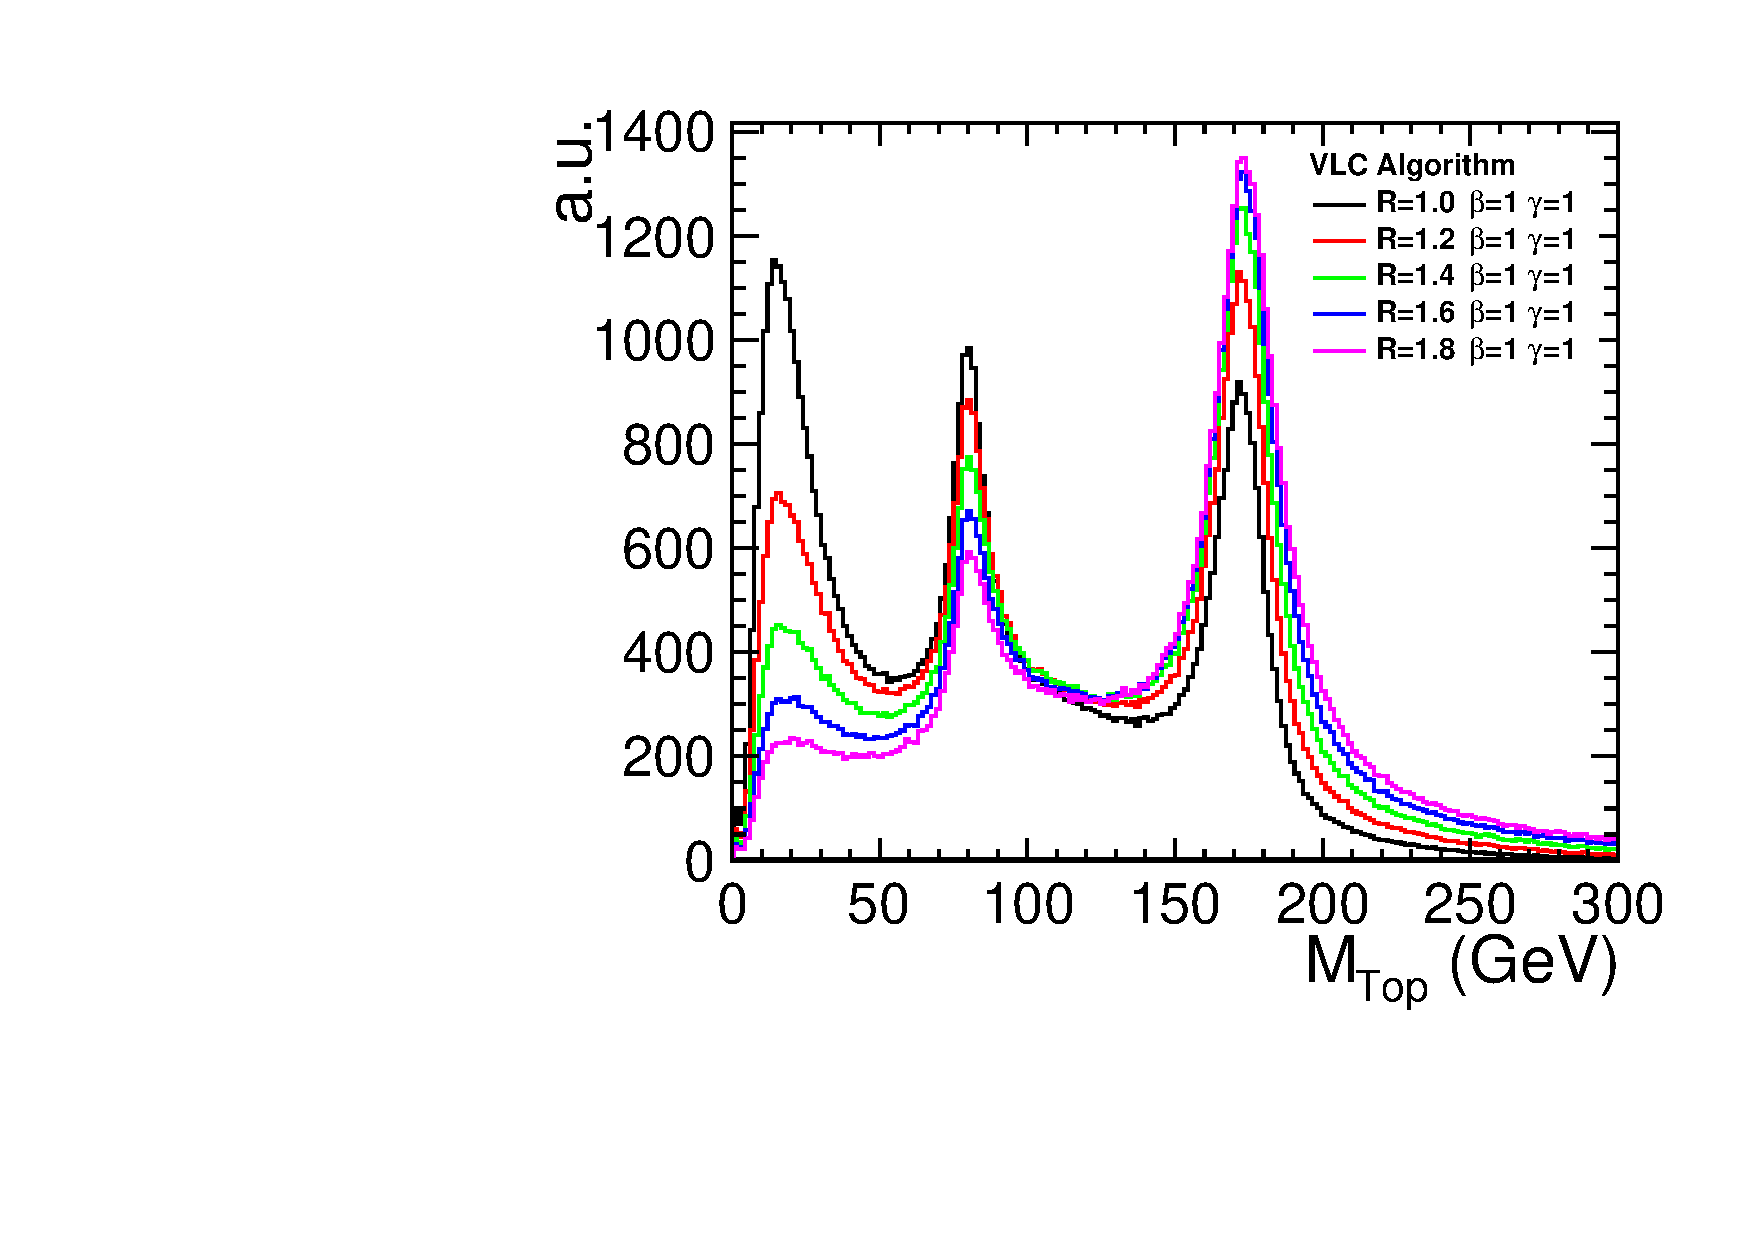
\includegraphics[width=1.0\textwidth]{TopAnalysis/figures/ComparisonVLC.pdf}
    \caption[Valenica algorithm]{Valencia algorithm}
  \end{subfigure}
  \caption[Performance of jet finding algorithms]{Performance of both jet finding algorithms for various parameter settings. The kt algorithm is seen to produce a broader distribution in the top mass peak so the Valencia algoritm is prefered. For both methods it is seen that a lower R results in the development of peaks from partial reconstruction of the top jet (W Boson or single quark) while a larger R produces a broader peak at the top mass. A balance is found between producing a narrow top mass width while minimising sub peaks by selecting a radius of R=1.5 }
  \label{fig:jetfinding}
\end{figure}


\begin{figure}
  \centering
  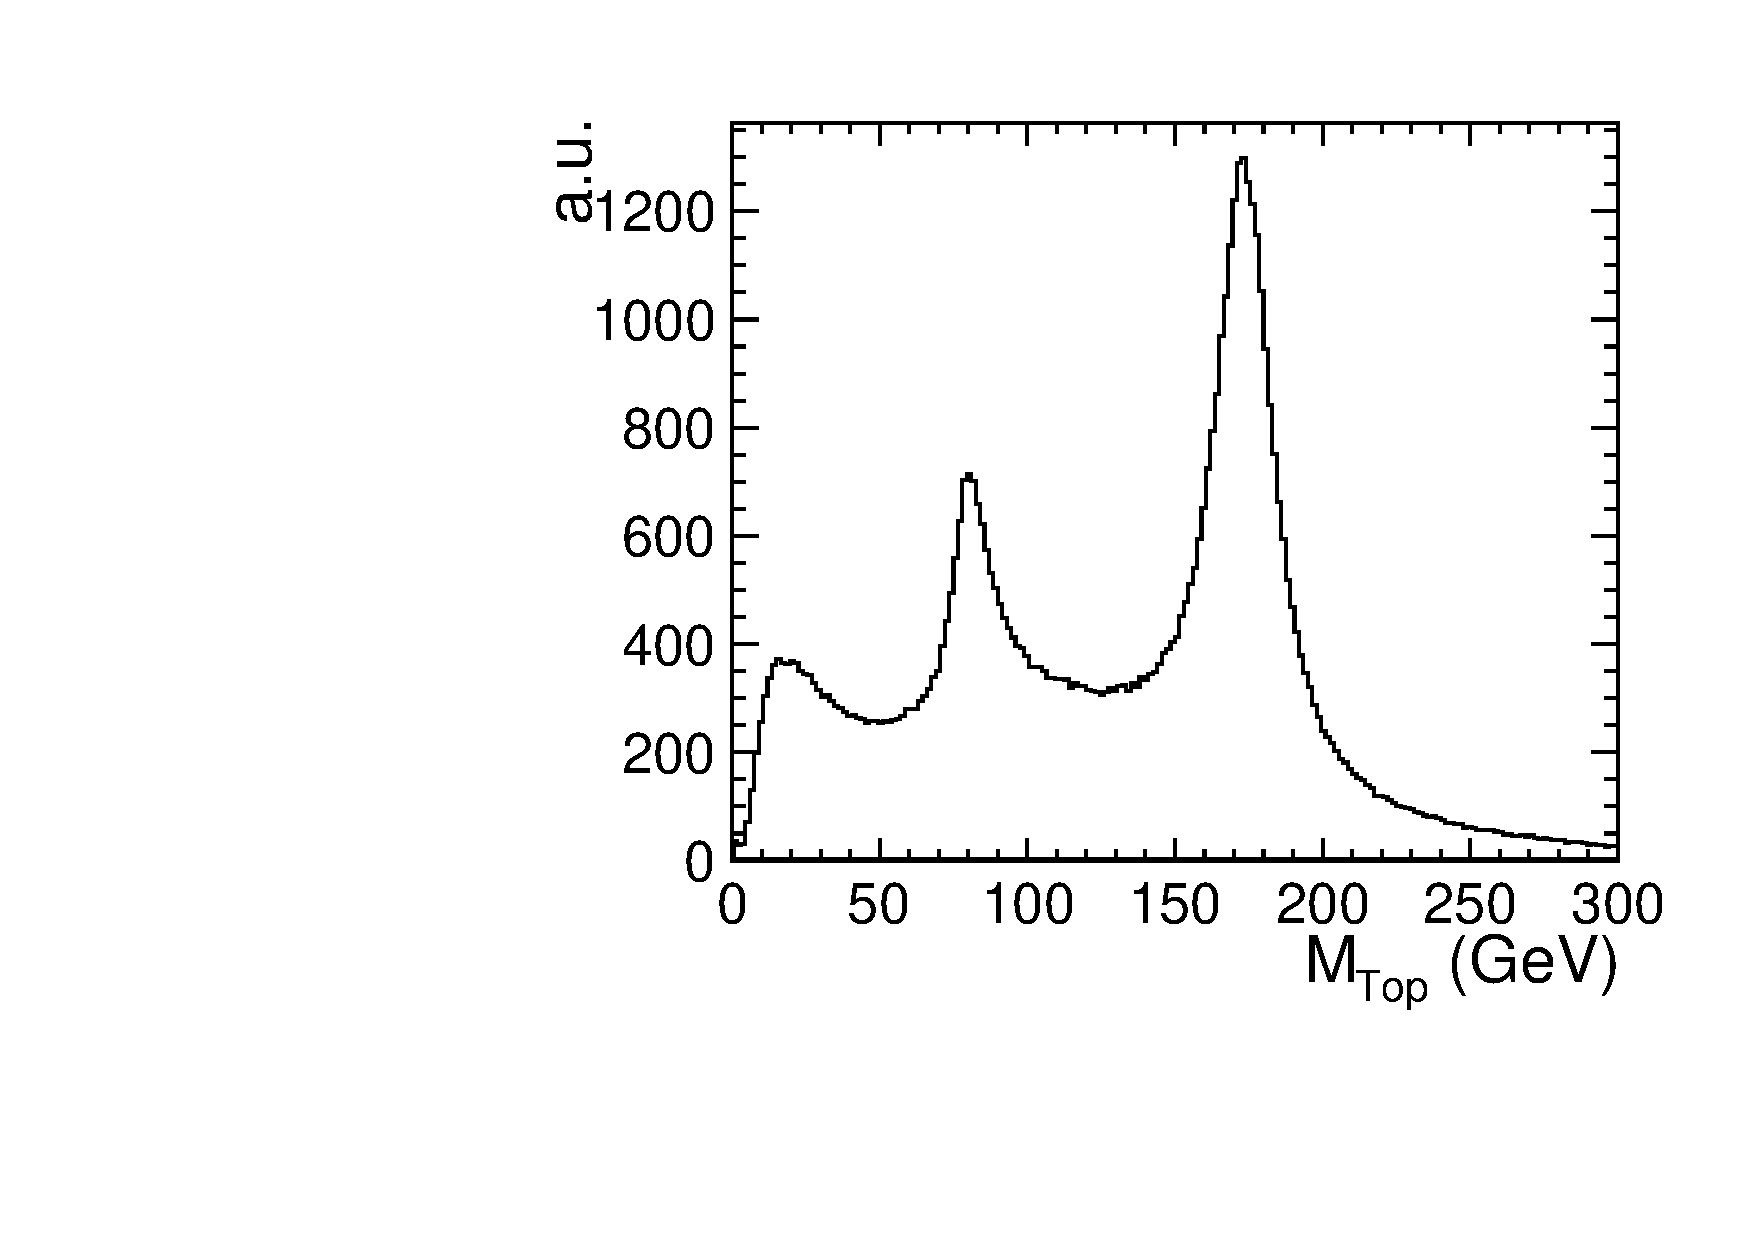
\includegraphics[width=0.7\textwidth]{TopAnalysis/figures/TopMass_EOver1200.pdf}
  \caption[Performance of Valencia algorithm for high energy events]{Reconstructed top mass for the Valencia algorithm in events close to the nominal collison energy (E $>$ 1.2~TeV)}
  \label{fig:highEValencia}
\end{figure}


\subsubsection{Jet Association}
\label{sec:jetassociation}
\begin{figure}
  \centering
  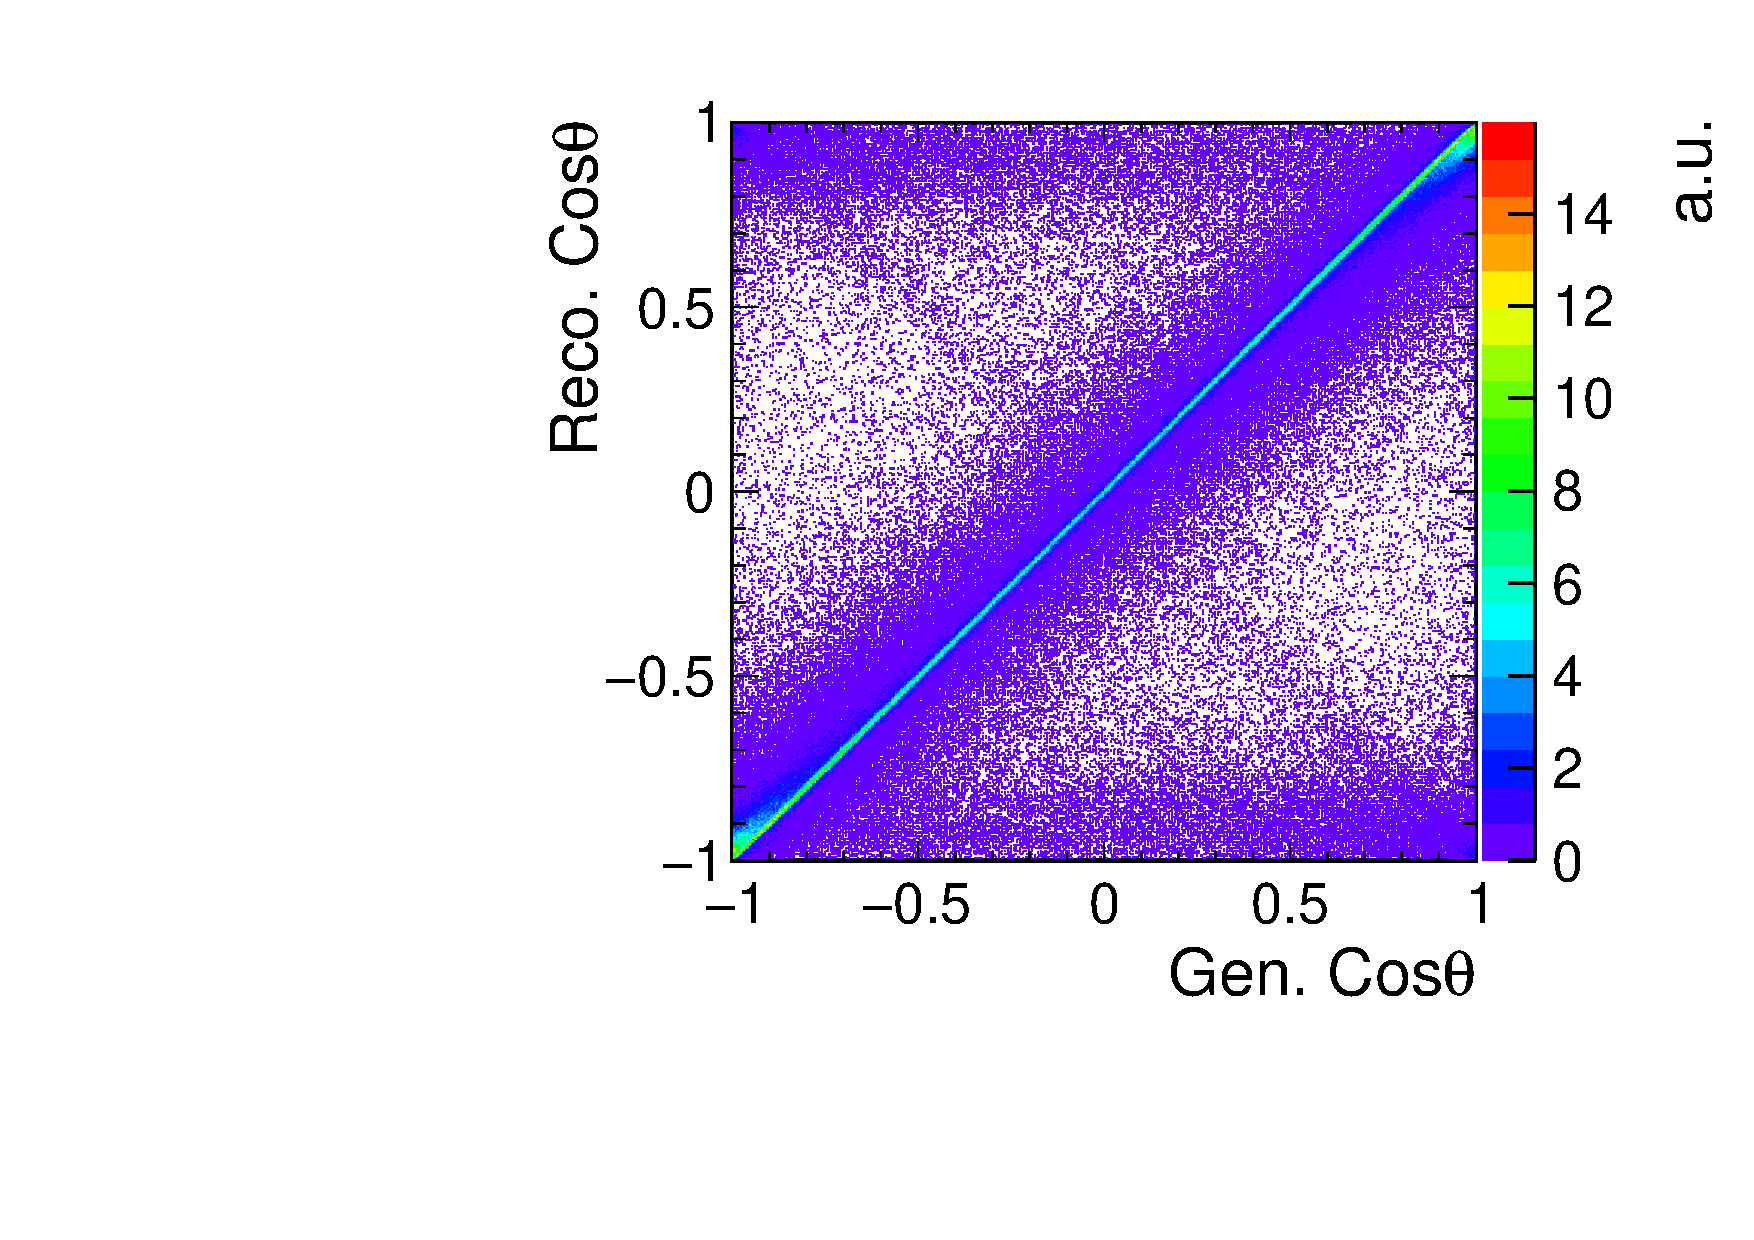
\includegraphics[width=0.7\textwidth]{TopAnalysis/figures/CosThetaRecoVsMC.pdf}
  \caption[Comparison of reconstructed top decay angle to generator level]{Comparison of reconstructed top decay angle to generator level. A strong correlation is seen over most of the range, however this starts to break down for large angles of $\mid cos\theta \mid>0.9$ where non-negligible off diagonal contributions are seen.}
  \label{fig:2djetangle}
\end{figure}

\begin{figure}
  \centering
  \begin{subfigure}{.5\textwidth}
    \centering
    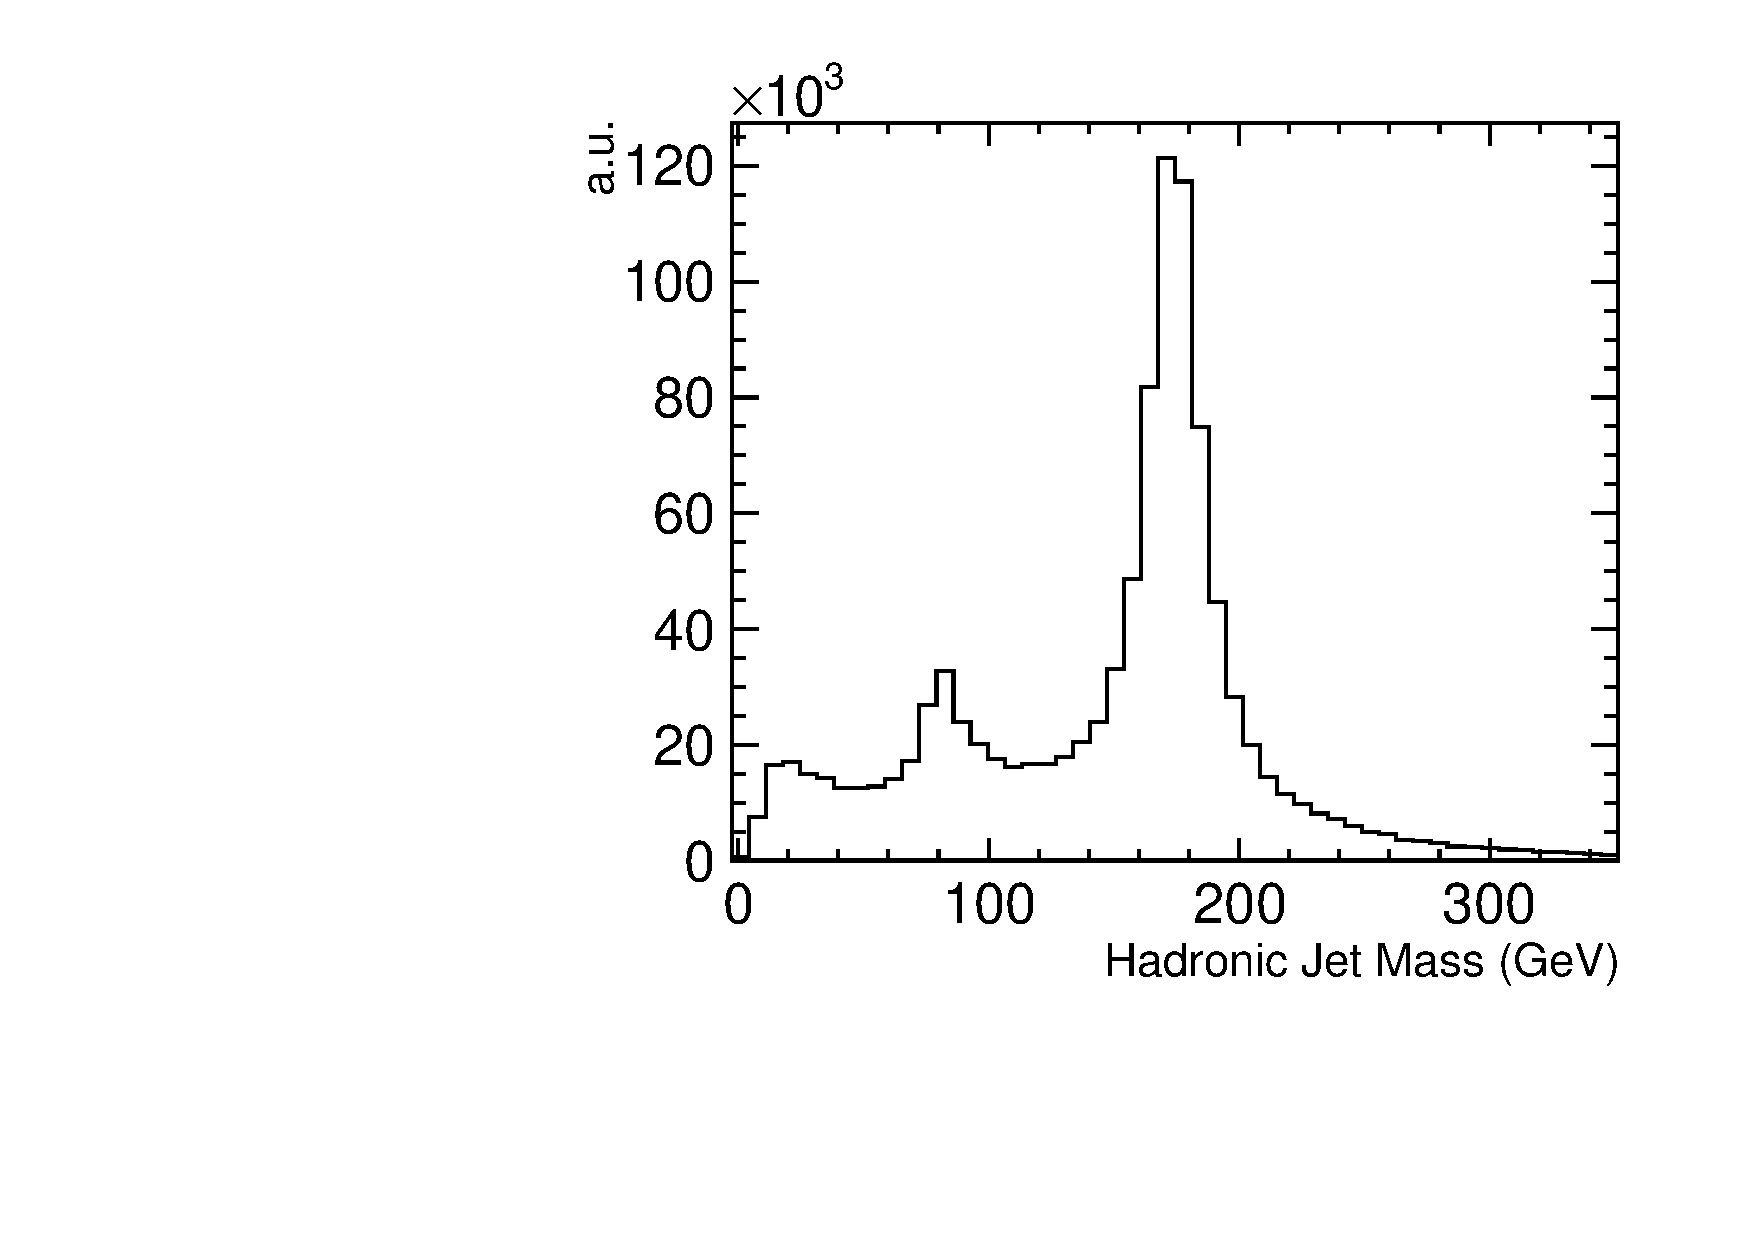
\includegraphics[width=1.0\textwidth]{TopAnalysis/figures/TopMassDiagonal.pdf}
  %  \caption[$\mid\frac{cos\theta_{Reco}}{cos\theta_{Generator}}\mid >1$]{Fat jet mass when $\mid\frac{cos\theta_{Reco}}{cos\theta_{Generator}}\mid >1$, on diagonal regions of fig \ref{fig:2djetangle}.}
  \end{subfigure}%
  \begin{subfigure}{.5\textwidth}
    \centering\captionsetup{width=.8\linewidth}%
    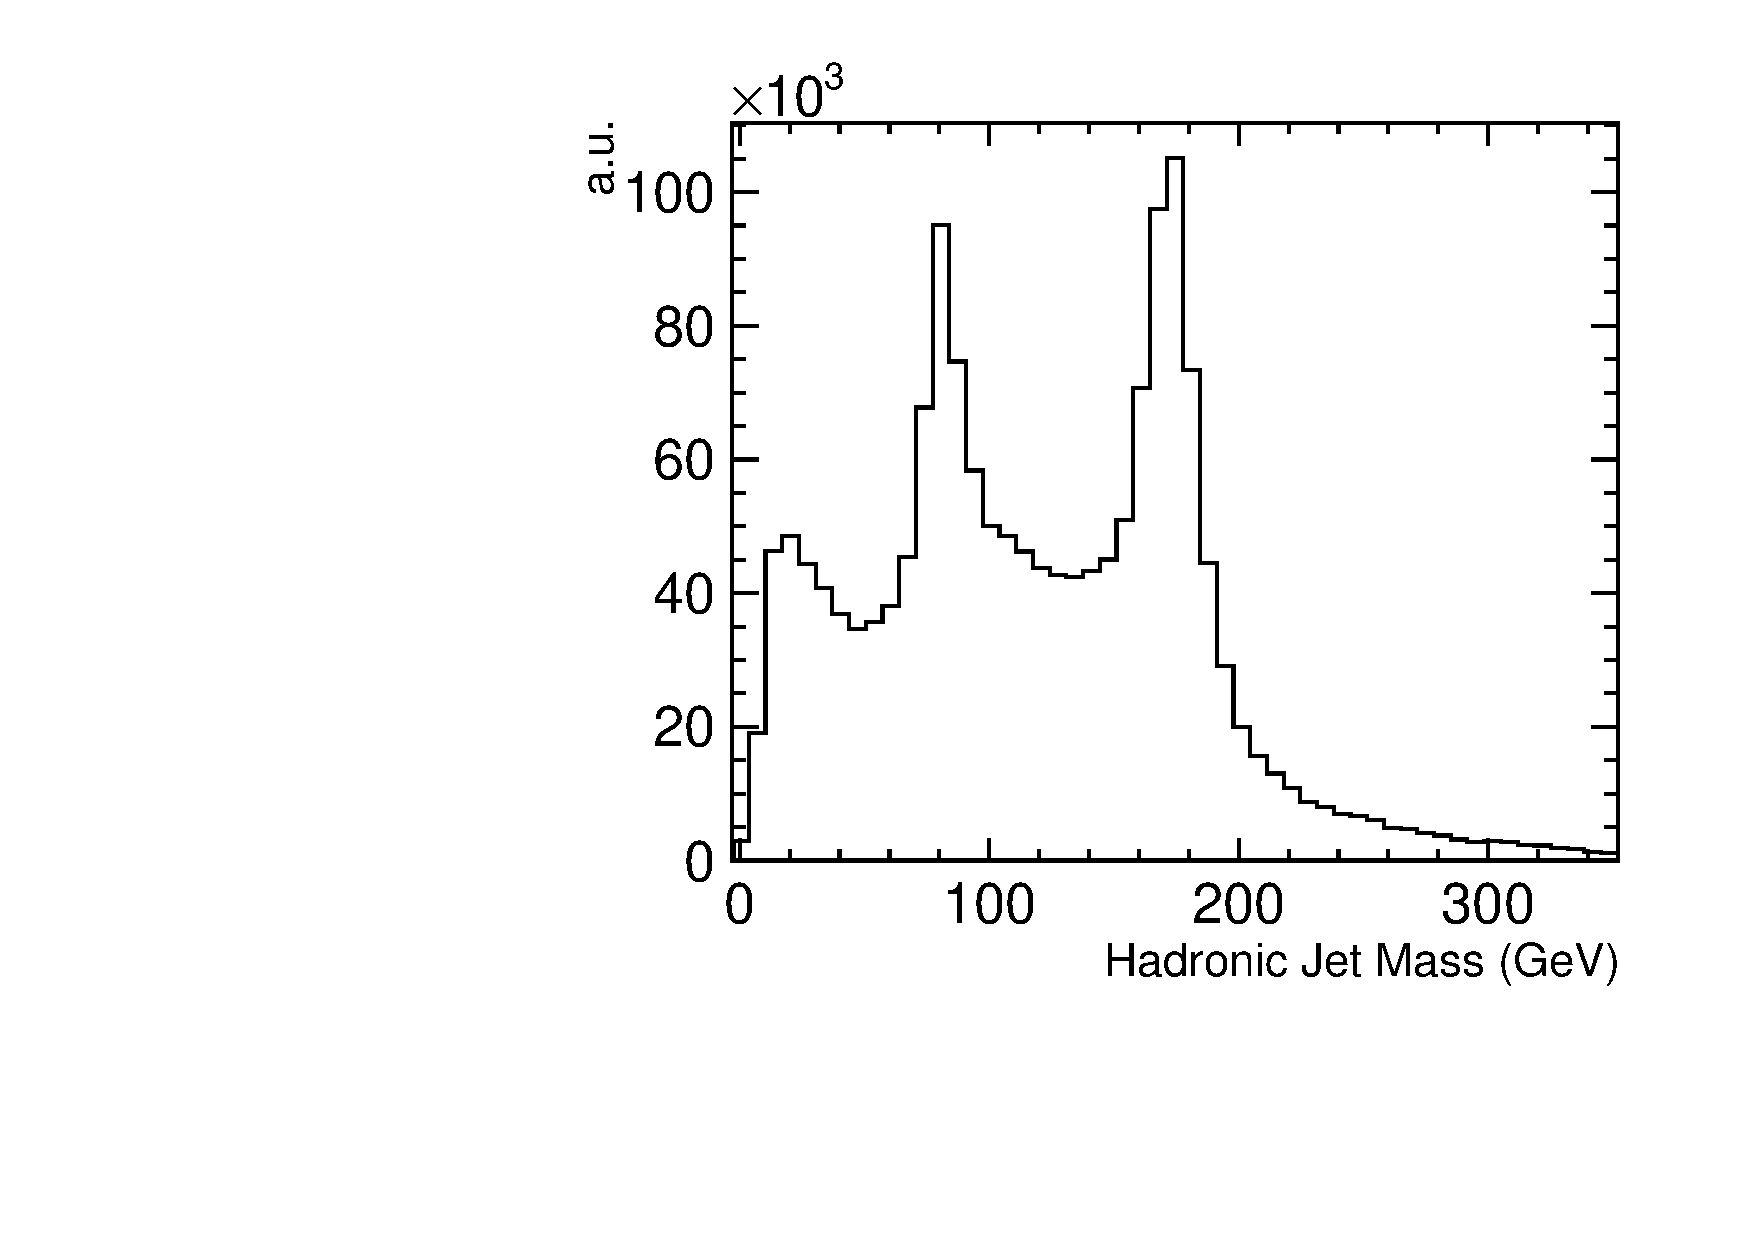
\includegraphics[width=1.0\textwidth]{TopAnalysis/figures/TopMassOffDiagonal.pdf}
 %   \caption[$\mid\frac{cos\theta_{Reco}}{cos\theta_{Generator}}\mid >1$]{Fat jet mass when $\mid\frac{cos\theta_{Reco}}{cos\theta_{Generator}}\mid <1$, off diagonal regions of fig \ref{fig:2djetangle}.}
  \end{subfigure}
  \caption[Reconstructed fat jet mass]{Reconstructed fat jet mass. In the on diagonal elements of \reffig{fig:2djetangle}) where $\mid\frac{cos\theta_{Reco}}{cos\theta_{Gen.}}\mid >1$ (left) the reconstructed fat jet matches the top mass, while in the regions corresponding to the off diagonal regions of \reffig{fig:2djetangle}) (right) the mass is no longer consistent.}
  \label{fig:diagonalTopMass}
\end{figure}


After the fat jet finding has been performed, the two reconstructed jets must then be associated as either coming from the hadronically decaying top or from the b jet from the leptonically decaying top. The default method for this was to associate the highest energy fat jet to the hadronically decaying top as, due to the neutrino not being reconstructed and the lepton already being removed, the remaining decay products from the leptonically decaying top should typically have considerably less energy. The performance of this method can be examined by comparing the reconstructed decay angle relative to the generator value (see \reffig{fig:2djetangle}). While the performance over most of the range studied is good, for $\mid cos\theta \mid>0.9$ the correlation between the generator and reconstructed angles breaks down and off diagonal elements start to appear. Performance in these forward regions is typically poor due to the detector acceptance which result in losses down the beam line. In cases where parts of the hadronic top decay are not able to be reconstructed, using the fat jets energy to perform the jet association no longer becomes a reliable method. Evidence that misreconstruction is the source of these off diagonal elements is presented in \reffig{fig:diagonalTopMass} where it is clear that the fat jets in the off diagonal regions are not reconstructed with a consistent mass. When the jets are not fully reconstructed, it is more likely that the wrong jet is assigned to be from the hadronic top. When the wrong jet is selected the reconstructed angle will be approximately $\pi$ radians off the generator value as the tops are predominantly produced back to back. This explanation is further supported by the results shown in \reffig{fig:2djetangle_farfromleptop} which show that the off diagonal elements can be removed when a cut is placed on the angle between the reconstructed top and the generator level b jet from the leptonic top decay indicating that these elements are definitely coming from selecting the wrong jet being selected. As well as the $\pi$ radian flips from selecting the wrong jet, there are also additional off diagonal contributions seen which arise from poor reconstruction of the fat jets. This typically happens when the tops are not produced back to back due to \ac{ISR}/\ac{BS}. When this happens, during the fat jet reconstruction it is possible for contributions from both true fat jets to be mixed e.g instead of grouping the 3 jets from the hadronic jets together only two of them are grouped together and the third is grouped with the lone b jet from the leptonic top. When this mismatching happens the hadronic top is no longer fully reconstructed and so the angle measured for the top decay has little correlation with the generator value. \reffig{fig:2djetangle_goodtopseparation} shows that these remaining off diagonal elements disappear when a cut is placed on the separation of the tops at truth level. 

\begin{figure}
  \centering
  \begin{subfigure}{.48\textwidth}
    \centering
    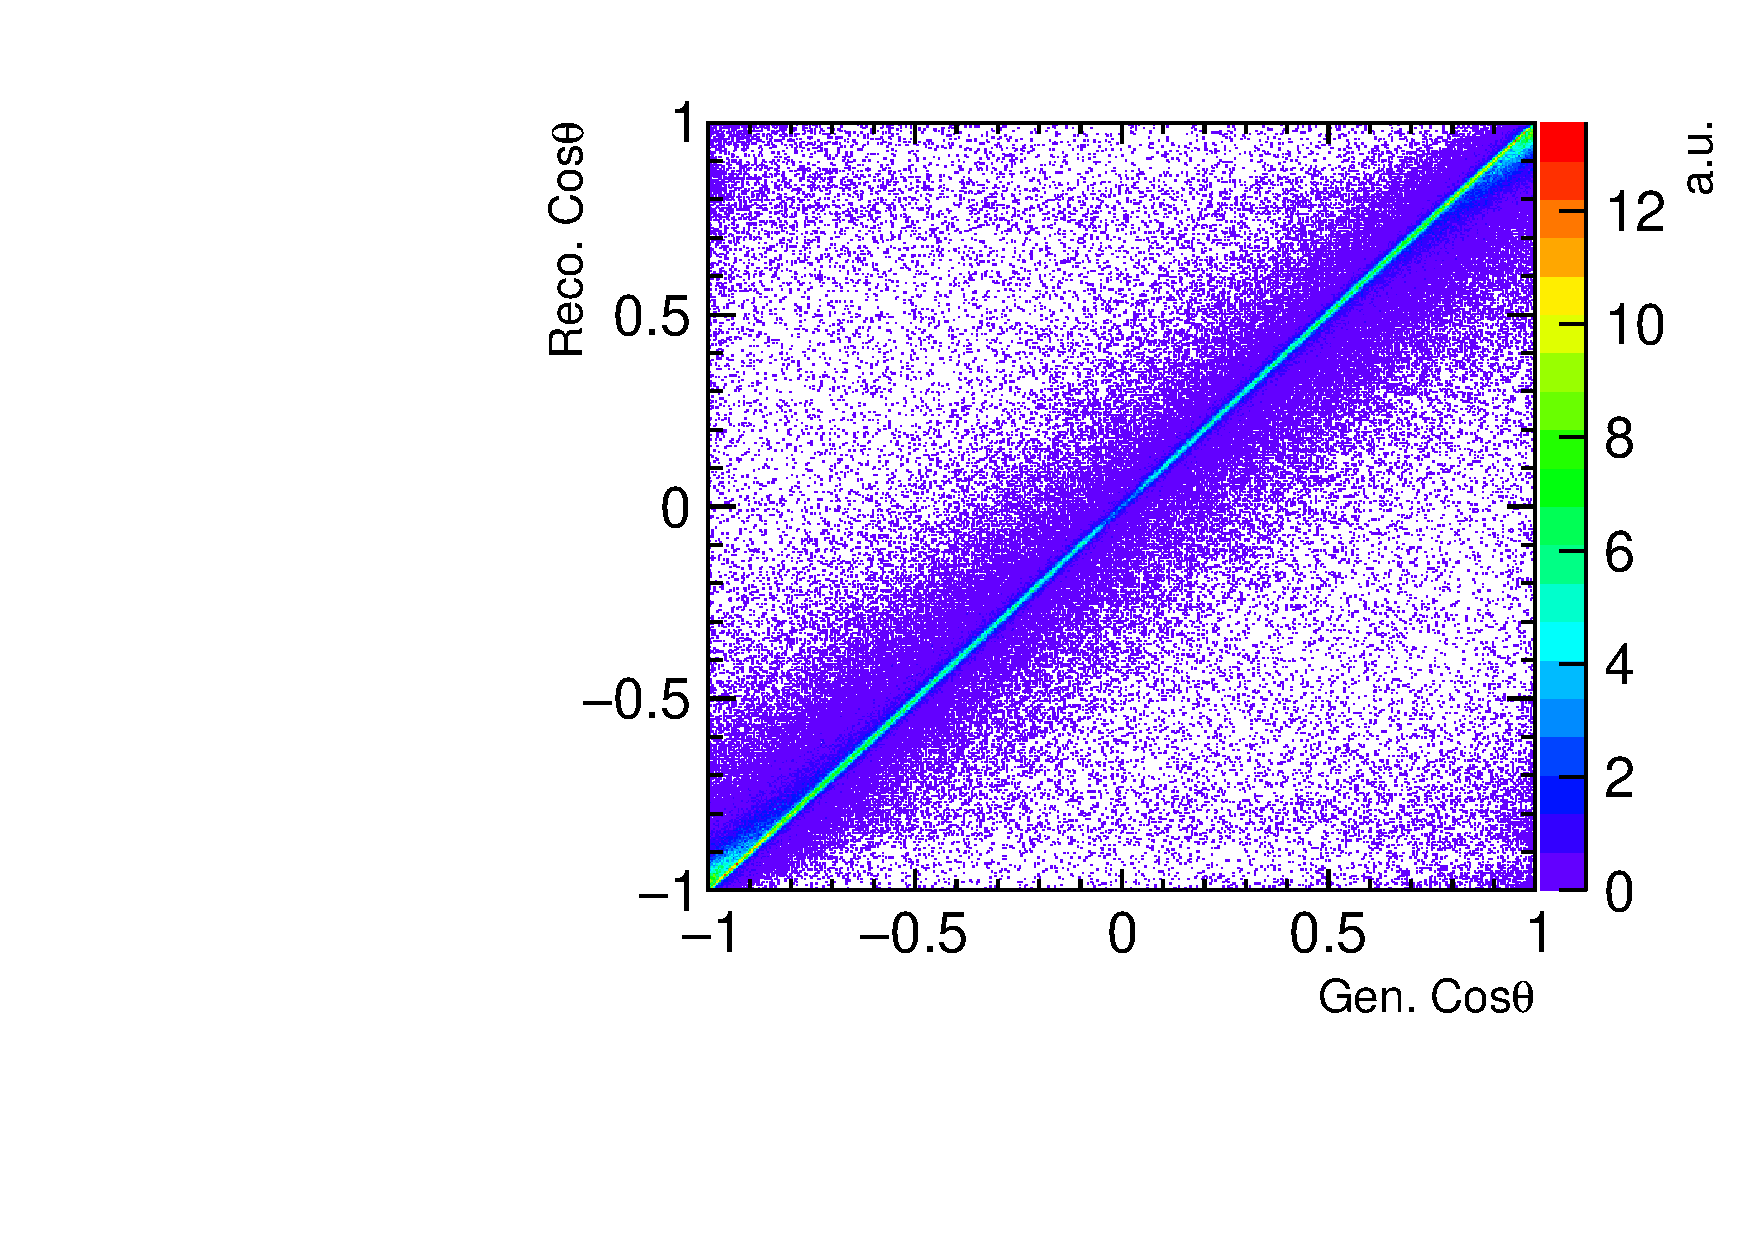
\includegraphics[width=1.0\textwidth]{TopAnalysis/figures/CosThetaRecoVsMC_NotNextToLepTop.pdf}%
    \caption[Cut placed on angle between reconstructed top and generator b jet from leptonic decay]{Cut placed on angle between reconstructed top and generator b jet from leptonic decay, $\Delta Cos\theta_{Reco-Bjet}>0.1$}
    \label{fig:2djetangle_farfromleptop}
  \end{subfigure}\hfill
  \begin{subfigure}{.48\textwidth}
    \centering
    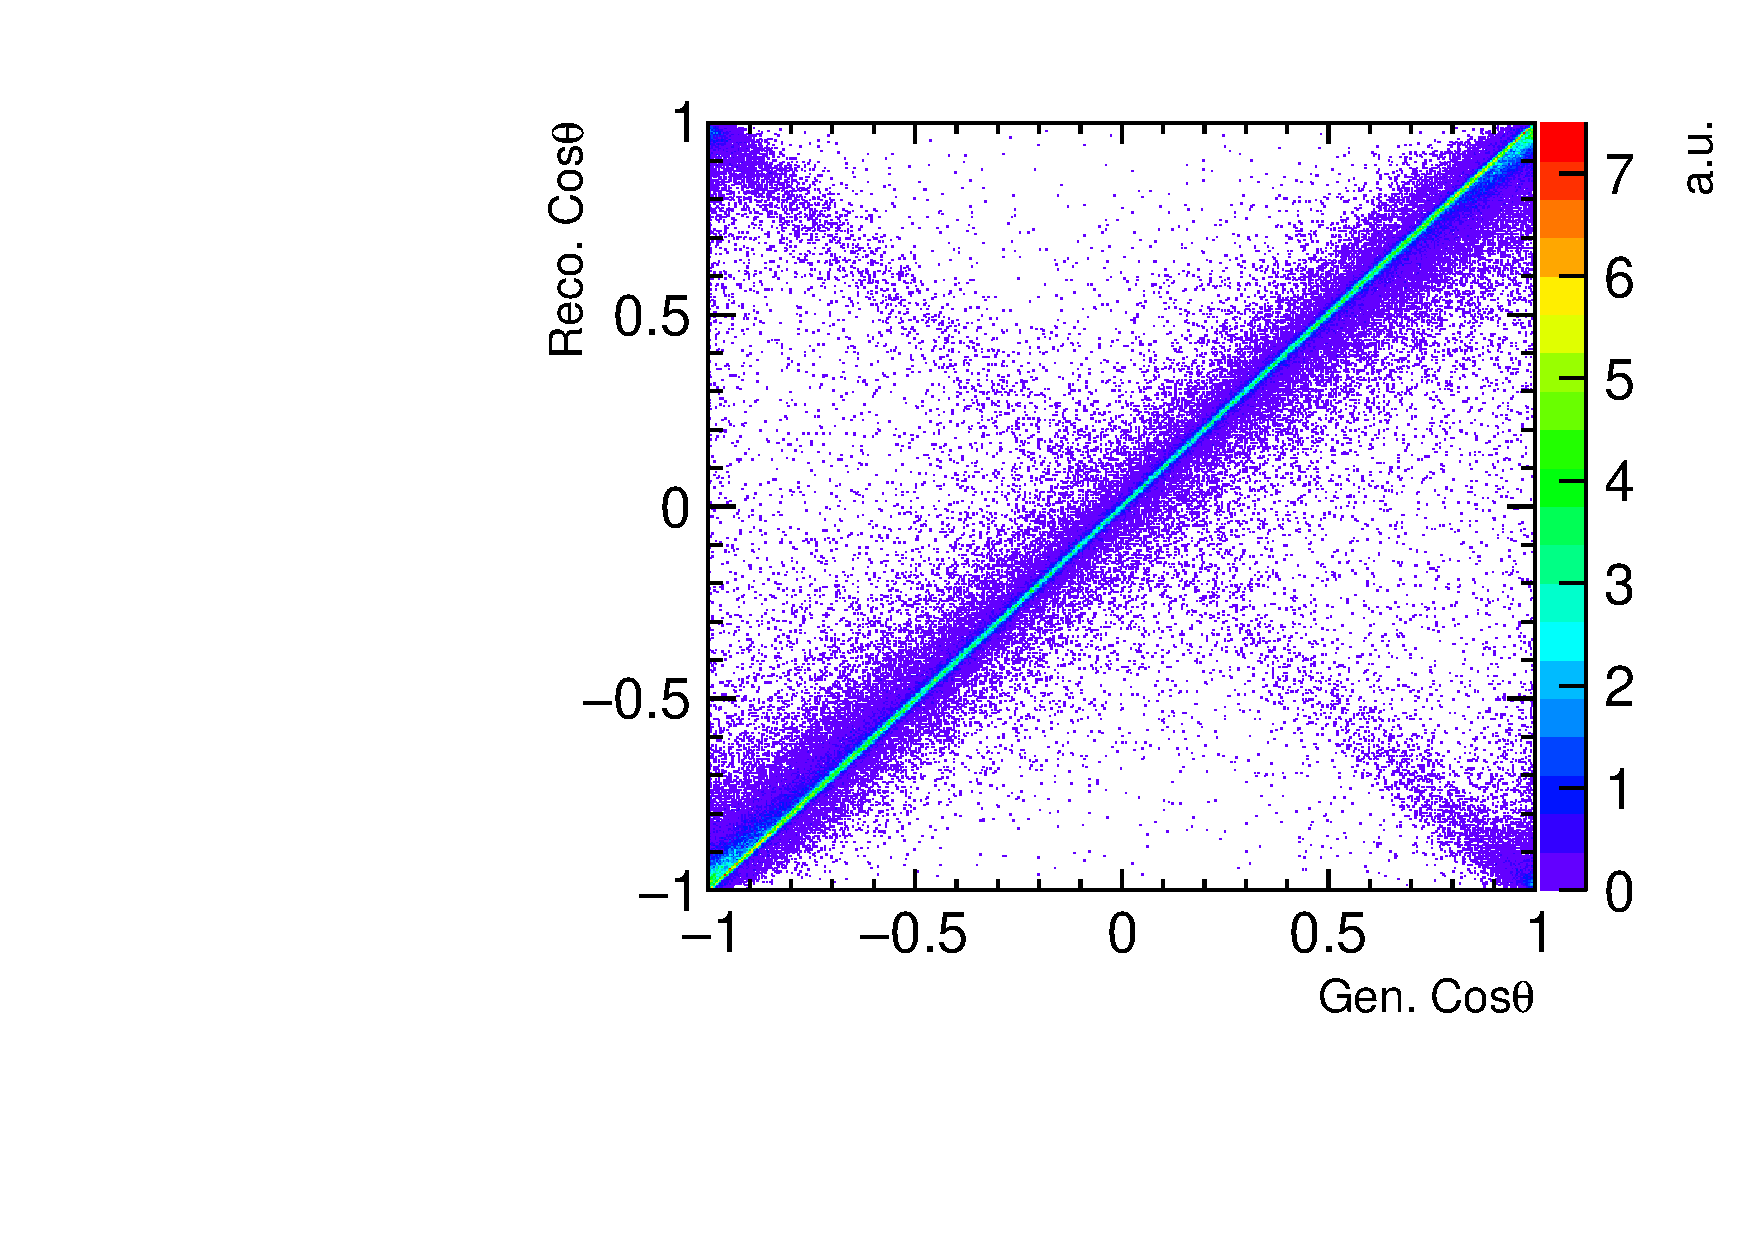
\includegraphics[width=1.0\textwidth]{TopAnalysis/figures/CosThetaRecoVsMC_MCTopsWellSeparated.pdf}%
    \caption[Cut placed on collinearity between top pair at generator level]{Cut placed on collinearity between top pair at generator level, separation $>$ 3 radians}
    \label{fig:2djetangle_goodtopseparation}
  \end{subfigure}
  \caption[Reconstructed vs generator top decay angles with truth level cuts]{Reconstructed vs generator top decay angles with truth level cuts to explain the off diagonal elements seen in \ref{fig:2djetangle}.}
  \label{fig:2djetangle_explanations}
\end{figure}


In order to avoid the problems close to the beam line multiple alternative jet association methods were devised- see \reftab{tab:methodDescription}.
\begin{table}
  \centering
  \begin{tabular}{l |p{100mm}}
    \toprule
    Fat Jet Selection Method     & Description  \\
    \midrule
    Lepton & The hadronically decaying top is deemed to be the fat jet with the greatest angular separation from the isolated lepton\\
    \midrule
    B tag & The hadronically decaying top is deemed to be the fat jet with the greatest angular separation from the jet with the highest b tag (see \ref{Flavour Tagging} for details on how flavour tagging is performed)\\
    \midrule
    Energy & Select the fat jet with the highest energy to be the hadronically decaying top\\
    \midrule
    Multiplicity & Recluster both fat jets into N ``micro jets'' (see \ref{Jet Multiplicity} for methodology) The hadronically decaying top should have a higher number of micro jets found within it\\
    \midrule
    Mass & The hadronically decaying top is deemed to be the fat jet with the greatest mass \\
    \midrule
    Top Mass & Select the fat jet whos mass is closest to the top mass as the hadronically decaying top \\
    \midrule
    Democratic & A combination of the lepton, energy and mass methods. Each method votes for which fat jet it thinks is the hadronically decaying top. The fat jet with the most votes is then selected as the hadronically decaying top  \\
    \bottomrule
  \end{tabular}
  \caption{Methods used for identifying which fat jet corresponds to the hadronically decaying top.}
  \label{tab:methodDescription}
\end{table}

The relative effectiveness of these methods were evaluated in three ways shown in \reffigs{fig:methodComparison}, \ref{fig:angleFitDiff} and \ref{fig:angularEfficiency} respectively. The first method was to look at the overall distribution of cos$\theta$ produced by each method compared to the distribution at generator level as this is what will be used to extract $A_{fb}^{t}$. All the methods agree well with the generator distribution in the central region of the detector but diverge in the high $\mid cos\theta\mid$ region. This is mainly caused by the effect described above. Close to the beam line the jets aren't fully reconstructed, the jet association fails and the b jet from the leptonic side is selected rather than the hadronic top jet. This causes migrations from the forward region to the backward regions producing a deficit in the forward region and an excess in the backward region. Migrations do occur in the opposite direction too for the same reason, however because the top forward-backward asymmetry means tht more tops are produced in the forward region to begin with, the net migration is from forward to backward. The migrations are not always a shift of $\pi$ radians as one might expect. Instead the migrations occur from very close to the beam line to a broader range in the opposite direction. This is due to the fact that \ac{ISR}/\ac{BS} can mean the top pair aren't produced exactly back to back in the lab frame and because the b-jet produced by the leptonic decay is not exactly collinear with the the top decay axis. Comparing the methods we see that all the methods show similar levels of migration except for the btag method which shows the highest migration. This is attributed to the fact the highest btagged jet can sometimes be from the hadronic side even in events that are well reconstructed, and so the jet association will fail in more events than the other methods which only fail for events close to the beam line.

\begin{figure}
  \centering
  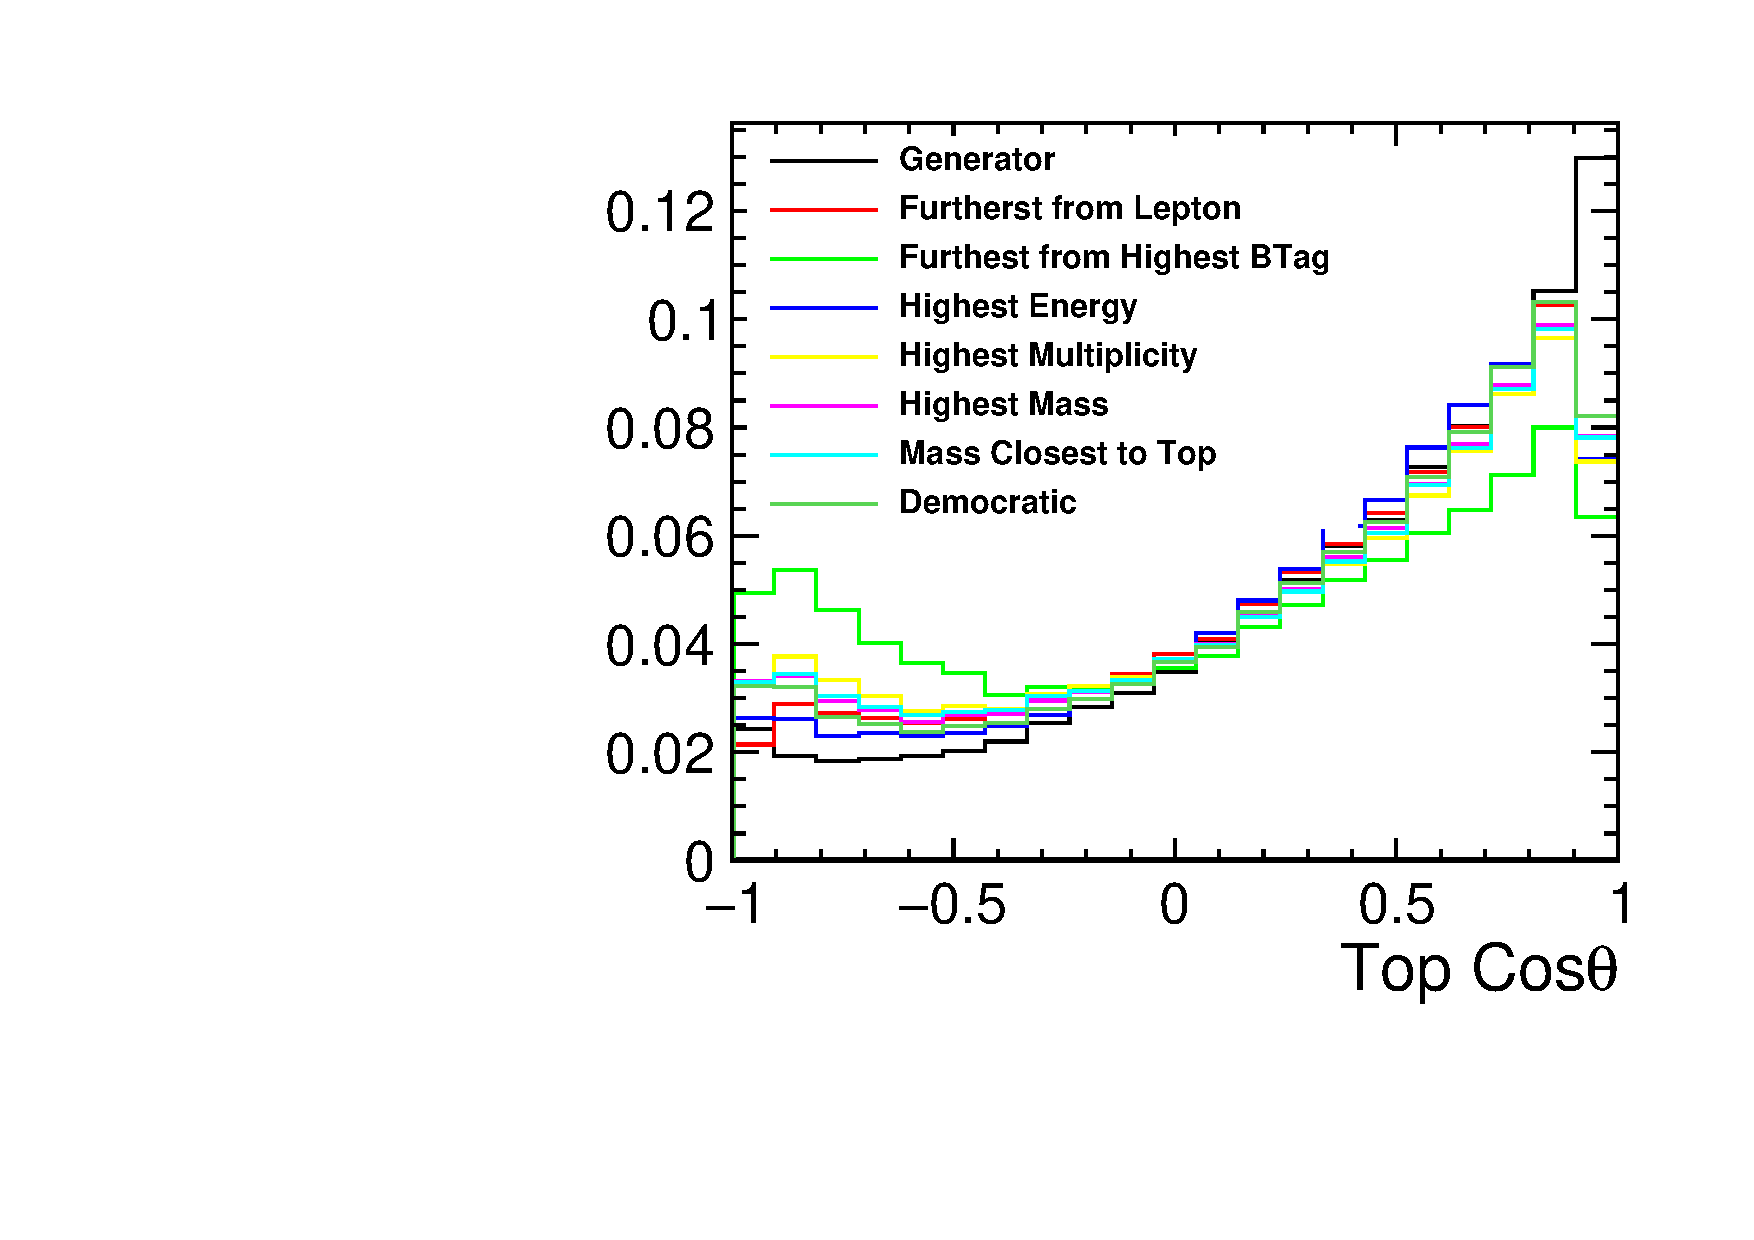
\includegraphics[width=0.6\textwidth]{TopAnalysis/figures/comparejetmethods.pdf}
  \caption[Reconstructed cos$\theta$ distribution for various jet association methods]{Reconstructed cos$\theta$ distribution for various jet association methods. The expected distribution from truth level information is uncluded for reference.}
  \label{fig:methodComparison}
\end{figure}

The second method was to measure the difference between the reconstructed and MC(generator) cos$\theta$ per event and fit this with a gaussian. The variation in the width and mean of these distributions were plotted against the generator cos$\theta$ and are shown in \reffig{fig:angleFitDiff}. The effects of migration at high cos$\theta$ is more pronounced in these plots where in the width we can see that the resolution on cos$\theta$ gets much worse in the forward regions and the mean shows a pull in opposite directions in these regions proving the migrations do indeed occur in both directions with the same rate. Unfortunately there is little discrimination seen between the methods except for showing that there are slightly larger migrations when using the b-tag method.

\begin{figure}
  \centering
  \begin{subfigure}{.5\textwidth}
    \centering
    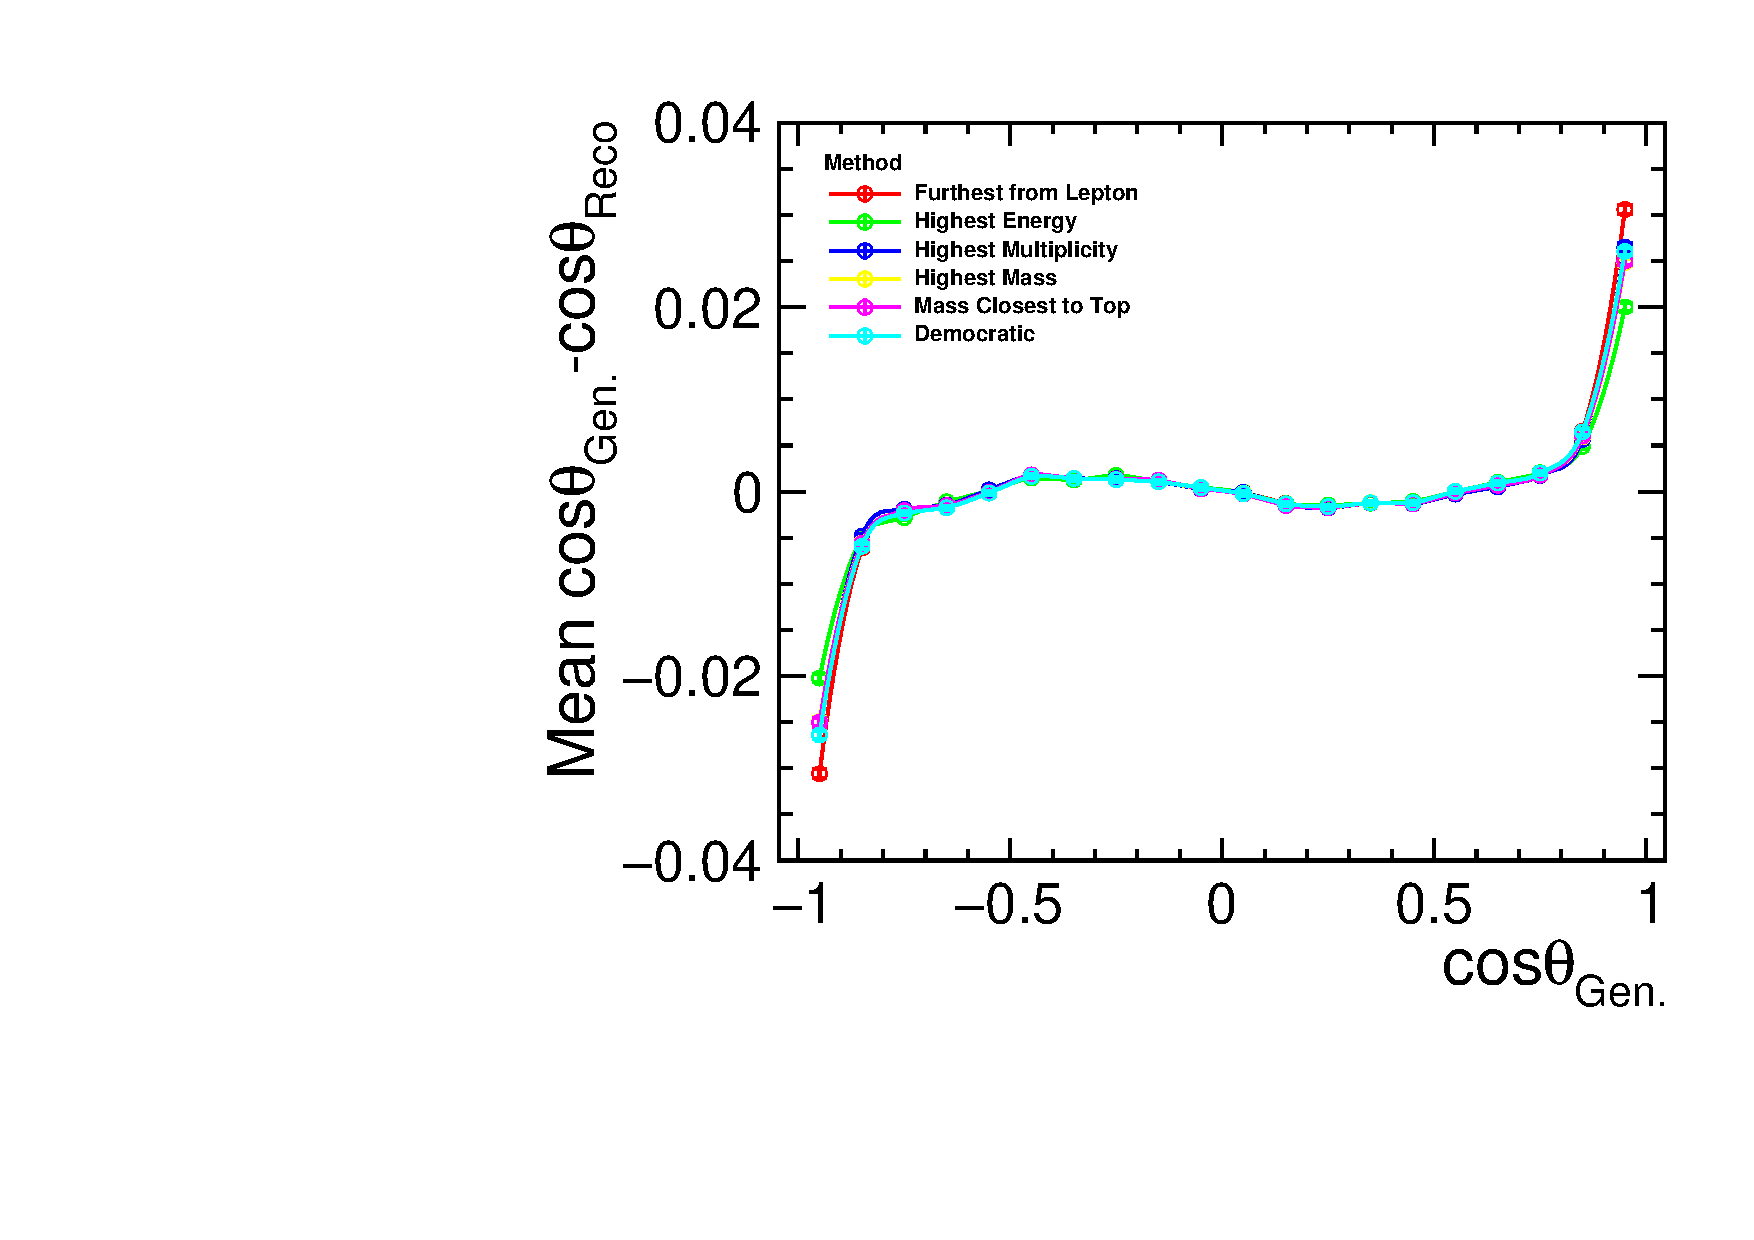
\includegraphics[width=0.9\textwidth]{TopAnalysis/figures/MeanThetaDiff.pdf}
    \caption[Mean]{Mean}
  \end{subfigure}%
  \begin{subfigure}{.5\textwidth}
    \centering
    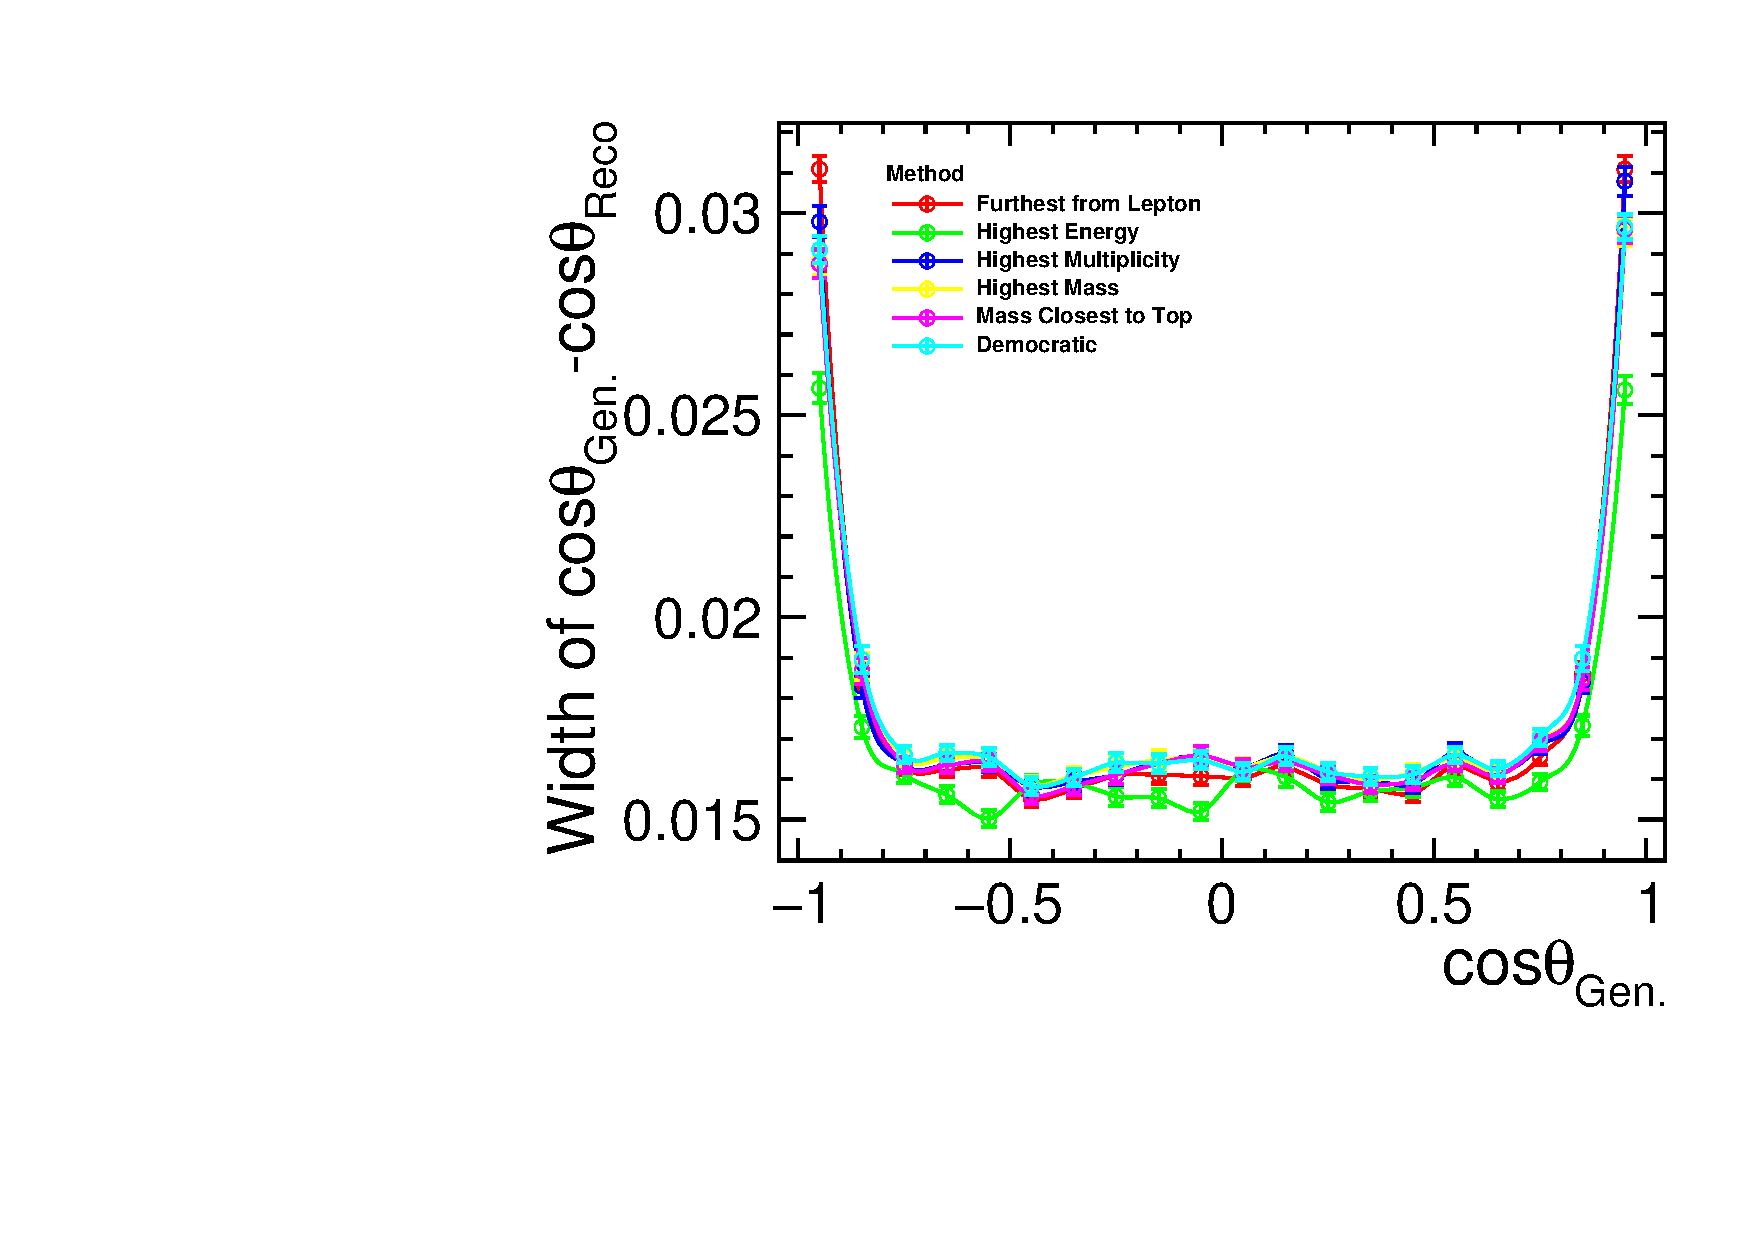
\includegraphics[width=0.9\textwidth]{TopAnalysis/figures/WidthThetaDiff.pdf}
    \caption[Width]{Width}
  \end{subfigure}
  \caption[Mean and width from fitting $\Delta cos\theta_{Gen.-Reco.}$ to a gaussian]{Mean and width from fitting $\Delta cos\theta_{Gen.-Reco.}$ to a gaussian. Mean: migrations close to $\mid cos\theta\mid>0.9$ result in a bias in the mean. The migrations cause a shift of roughly $\pi$ radians resulting in the bias being in the opposite direction for each end of the range. Width: migrations close to $\mid cos\theta\mid>0.9$ cause a broadening in the resolution of the reconstructed cos$\theta$.}
  \label{fig:angleFitDiff}
\end{figure}

The final method of comparison was to measure the efficiency with which the hadronic top was measured within the correct cos$\theta$ bin as a function of the generator cos$\theta$. For this study a bin width of 0.1 in cos$\theta$ was used. The results are shown in \reffig{fig:angularEfficiency}. Here there is a clearer separation in the performance of the different methods. B-tagging is seen to provide the worst efficiency while the energy and democratic methods provide the highest level of performance. The mass based selections provide slightly lower performance than the energy/democratic methods. This is likely explained by the fact they are less robust when the the event the jets are not fully reconstructed. Missing a small section of the jet via acceptance losses/reconstruction inefficiencies can have a large impact on the reconstructed mass, however in the case of energy, if we naively assume that the energy is split evenly between the 6 final state particles, then we would expect that the energy of the hadronic fat jet would be three times that of the b-jet from the leptonic top and so considerable energy losses must occur before the wrong jet is selected. Due to their higher bin by bin efficiency, the energy and democratic methods are the best methods to use. Due to it's simplicity the energy method is then chosen as the preferred method for the rest of the analysis. 

\begin{figure}
  \centering
  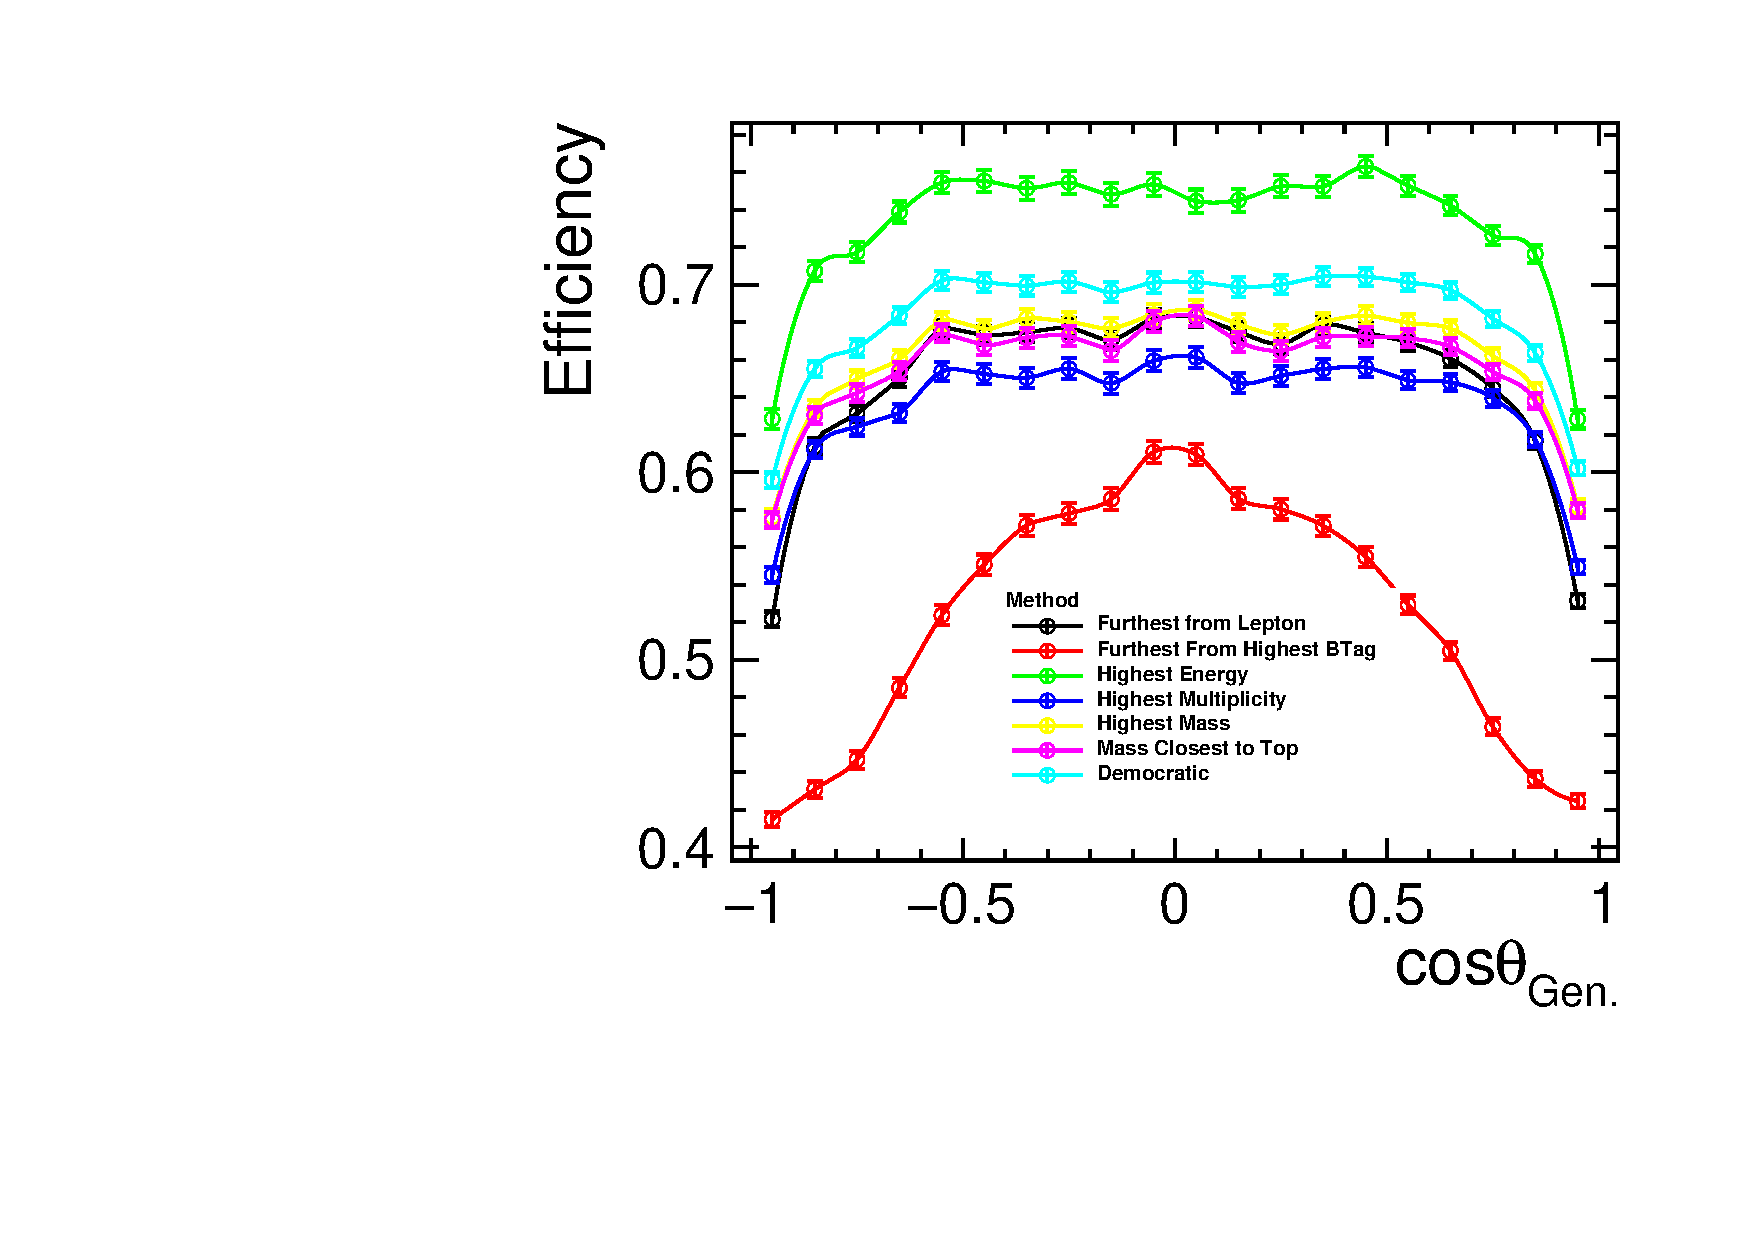
\includegraphics[width=0.6\textwidth]{TopAnalysis/figures/EfficiencyvsMCTheta.pdf}
  \caption[Efficiency for reconstructing the hadronically decaying top in the correct cos$\theta$ bin]{Efficiency for reconstructing the hadronically decaying top in the correct cos$\theta$ bin.}
  \label{fig:angularEfficiency}
\end{figure}

\subsection{Jet Substructure}

\subsubsection{NSubjettiness}
\subsubsection{Subjet Angular Distributions}
\subsubsection{Jet Multiplicity}
\label{Jet Multiplicity}




\subsection{S' Reconstruction}

\begin{figure}
  \centering
  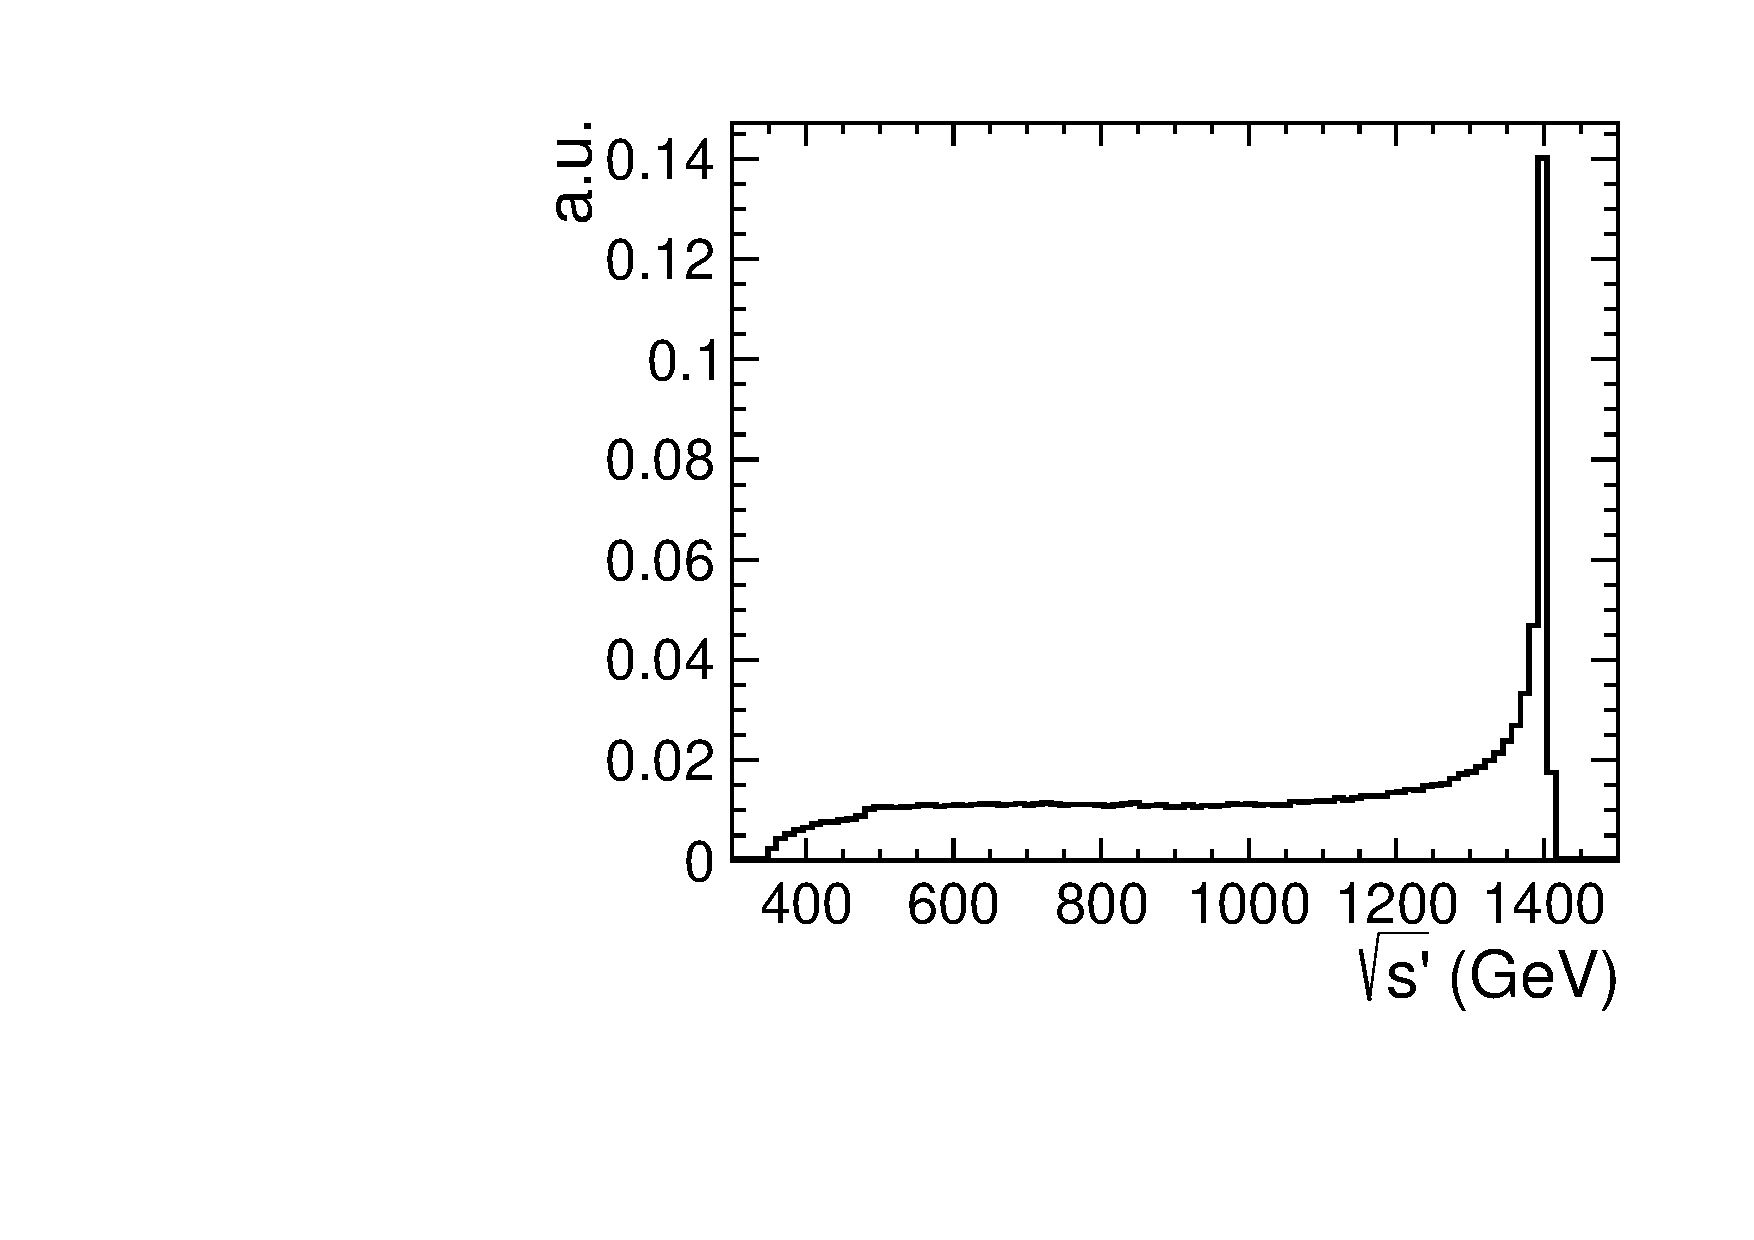
\includegraphics[width=0.6\textwidth]{TopAnalysis/figures/GeneratorSPrime.pdf}
  \caption[Expected s' spectrum for $t\bar{t}$ at 1.4~TeV]{Expected s' spectrum for $t\bar{t}$ at 1.4~TeV}
  \label{fig:trueSPrime}
\end{figure}

Following the reconstruction of the lepton and hadronically decaying top it is already possible to calculate $A_{FB}^{t}$, however there is still benefit to first reconstructing the effective centre-of-mass energy of the events (along with the neutrino and any photons produced too.) This allows the calculation of $A_{FB}^{t}$ to be determined in the $t\bar{t}$ rest frame where it is predicted to be up to 50\% larger \cite{Krohn:2011tw}, and also allows a differential measurement of $A_{FB}^{t}$ to be performed. The expected $\sqrt{s'}$ spectrum for $t\bar{t}$ production at 1.4~TeV is shown in \reffig{fig:trueSPrime}. Here it is seen that there is a large tail to the energy spectrum which can be taken advantage of to measure $A_{FB}^{t}$ over a large range of energies. This differential measurement provides greater power for discriminating between different physics models than a single $A_{FB}^{t}$ measurement. If s' can not be reconstructed per event, $A_{FB}^{t}$ would have to either be measured as an integral over the full s' range or be measured just around the peak energy where there are only small s' corrections (E $>$ 1200~GeV), however this would mean discarding $\sim$ 60\% of events produced during the 1.4~TeV run. As well as directly effecting the ways in which we can measure $A_{FB}^{t}$, reconstructing s' typically involves reconstructing the neutrino and photon contributions in the event. Having a description of these objects could provide further information by allowing the reconstruction of the leptonic top and so could help distinguish signal events from similar backgrounds.

In order to reconstruct s', multiple methods were attempted with varying complexity. In all cases, combined contributions from \ac{ISR} and \ac{BS} are approximated to the production of one photon radiated from the incoming electron positron pair.x

\subsubsection{Transverse/Longitudinal Association}

\begin{figure}
  \centering
  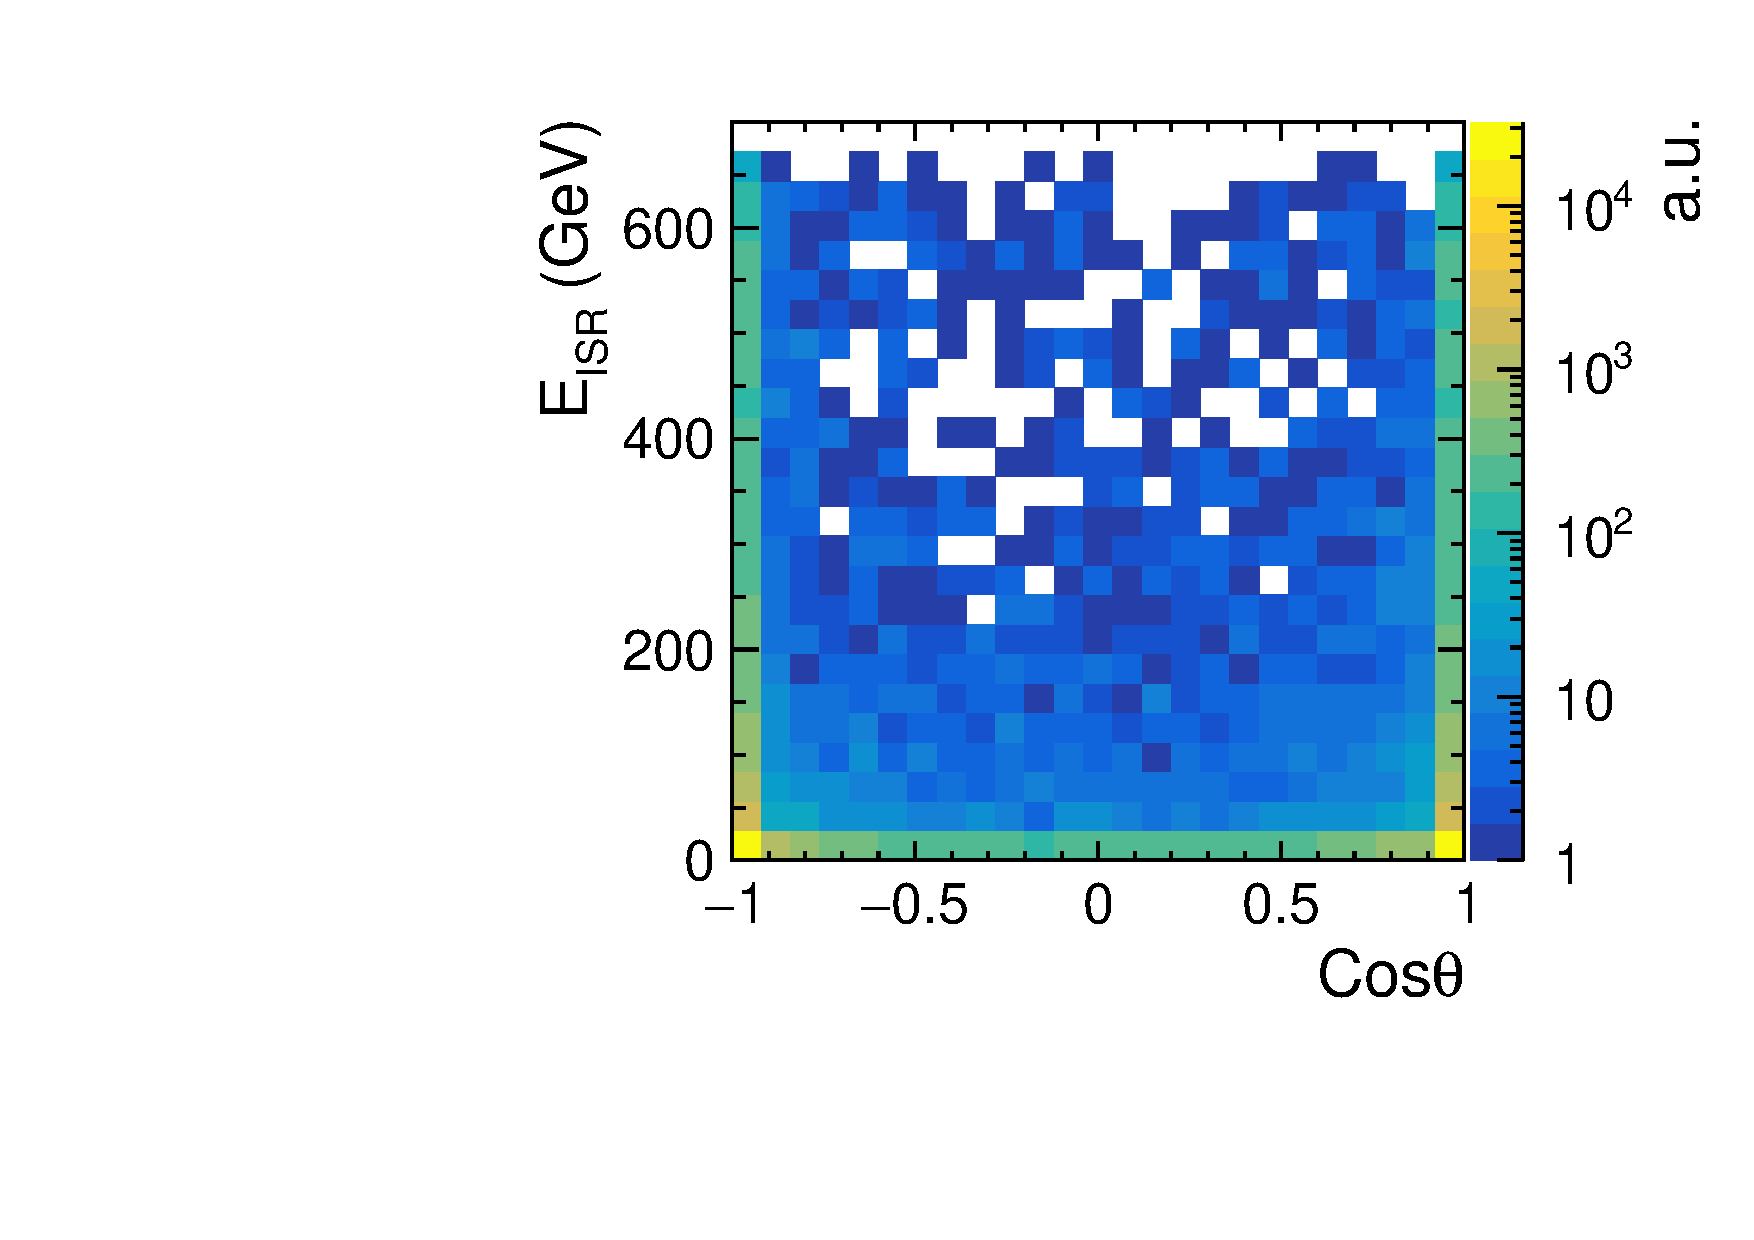
\includegraphics[width=0.6\textwidth]{TopAnalysis/figures/ISRSpectrum.pdf}
  \caption[Angular energy distribution of initial state photons]{Angular energy distribution of initial state photons}
  \label{fig:photonspectrum}
\end{figure}


The simplest method attempted was to assume that all missing momentum in the transverse direction is attributed to the neutrino, while all longitudinal missing momentum comes from photon contributions. These assumptions are motivated by the results from \reffig{fig:photonspectrum} which show that \ac{ISR} photons are predominantly produced collinear to the beam. Using this method s' is then taken to be the mass of the neutrino + fat jets system. An event by event comparison of the reconstructed s' to the generator s'is shown in \reffig{fig:simpleAssoication}. Overall this method is unsatisfactory as the reconstructed s' is consistently underestimating the true s' of the event. In retrospect this should be expected as the assumption that the photon losses are collinear to the beam is only approximately true. We have shown that it is true for high energy \ac{ISR} photons, however one can see from \reffig{fig:photonspectrum} that for lower energy emissions the photons can be emitted at large angles relative to the beam. This is why there is a stronger correlation between the reconstructed and generator s' when the photon energy losses are largest. On top of this there will also be photons produced through \ac{BS} and there is no reason to assume these would be produced with negligible transverse momentum. In practice the neutrino from the leptonic top decay will also have a non negligible longitudinal momentum that should be accounted for. Overall it is clear that this method is unsatisfactory for recobnstructing s'.

\begin{figure}
  \centering
  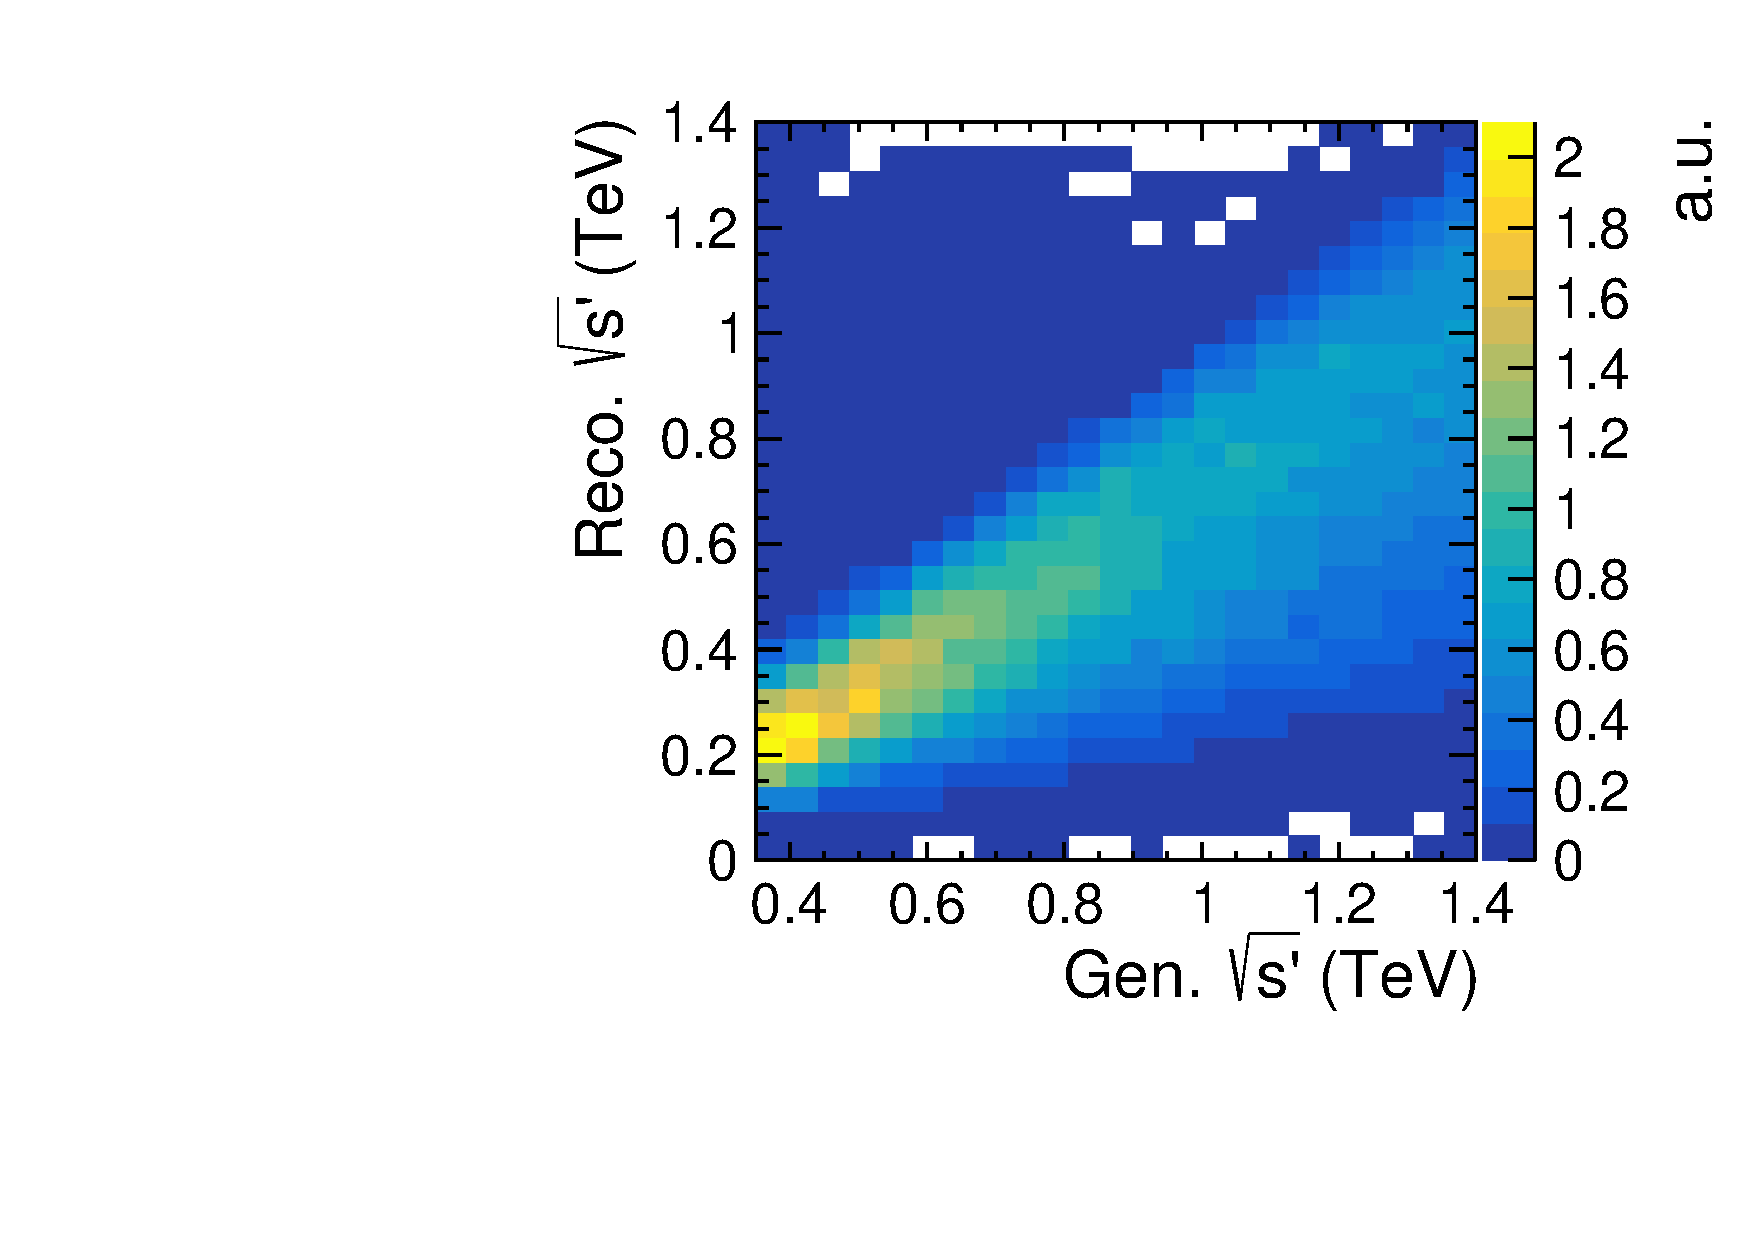
\includegraphics[width=0.6\textwidth]{TopAnalysis/figures/CrudeEVsTrueE.pdf}
  \caption[Reconstructed s' vs generator s' for Transverse/Longitudinal Association Method]{Reconstructed s' vs generator s' for Transverse/Longitudinal Association Method}
  \label{fig:simpleAssoication}
\end{figure}

\subsubsection{Analytic Mass Constraint}

\begin{figure}
  \centering
  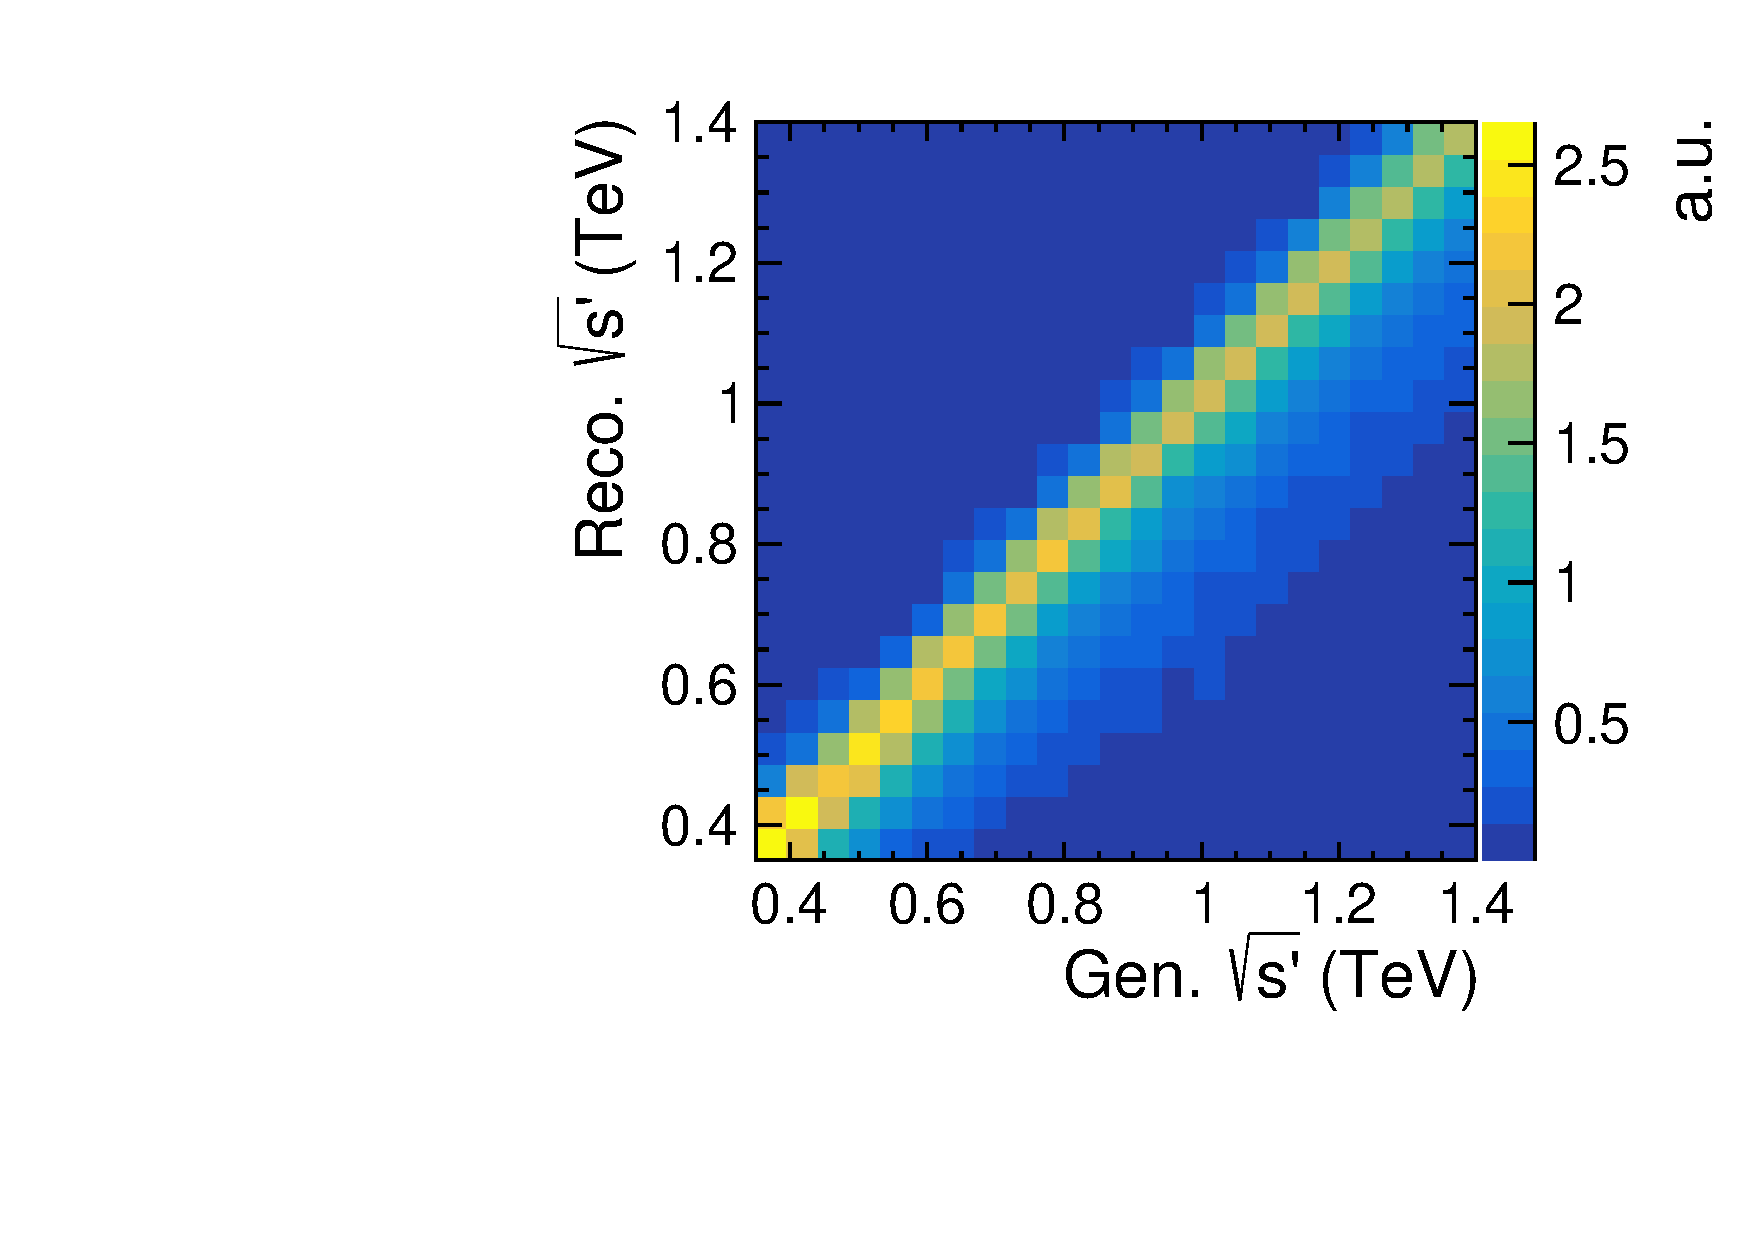
\includegraphics[width=0.6\textwidth]{TopAnalysis/figures/AnalEVsTrueE.pdf}
  \caption[Reconstructed s' vs generator s' for mass constraint method]{Reconstructed s' vs generator s' for mass constraint method}
  \label{fig:MassConstraint}
\end{figure}
\begin{figure}
  \centering
  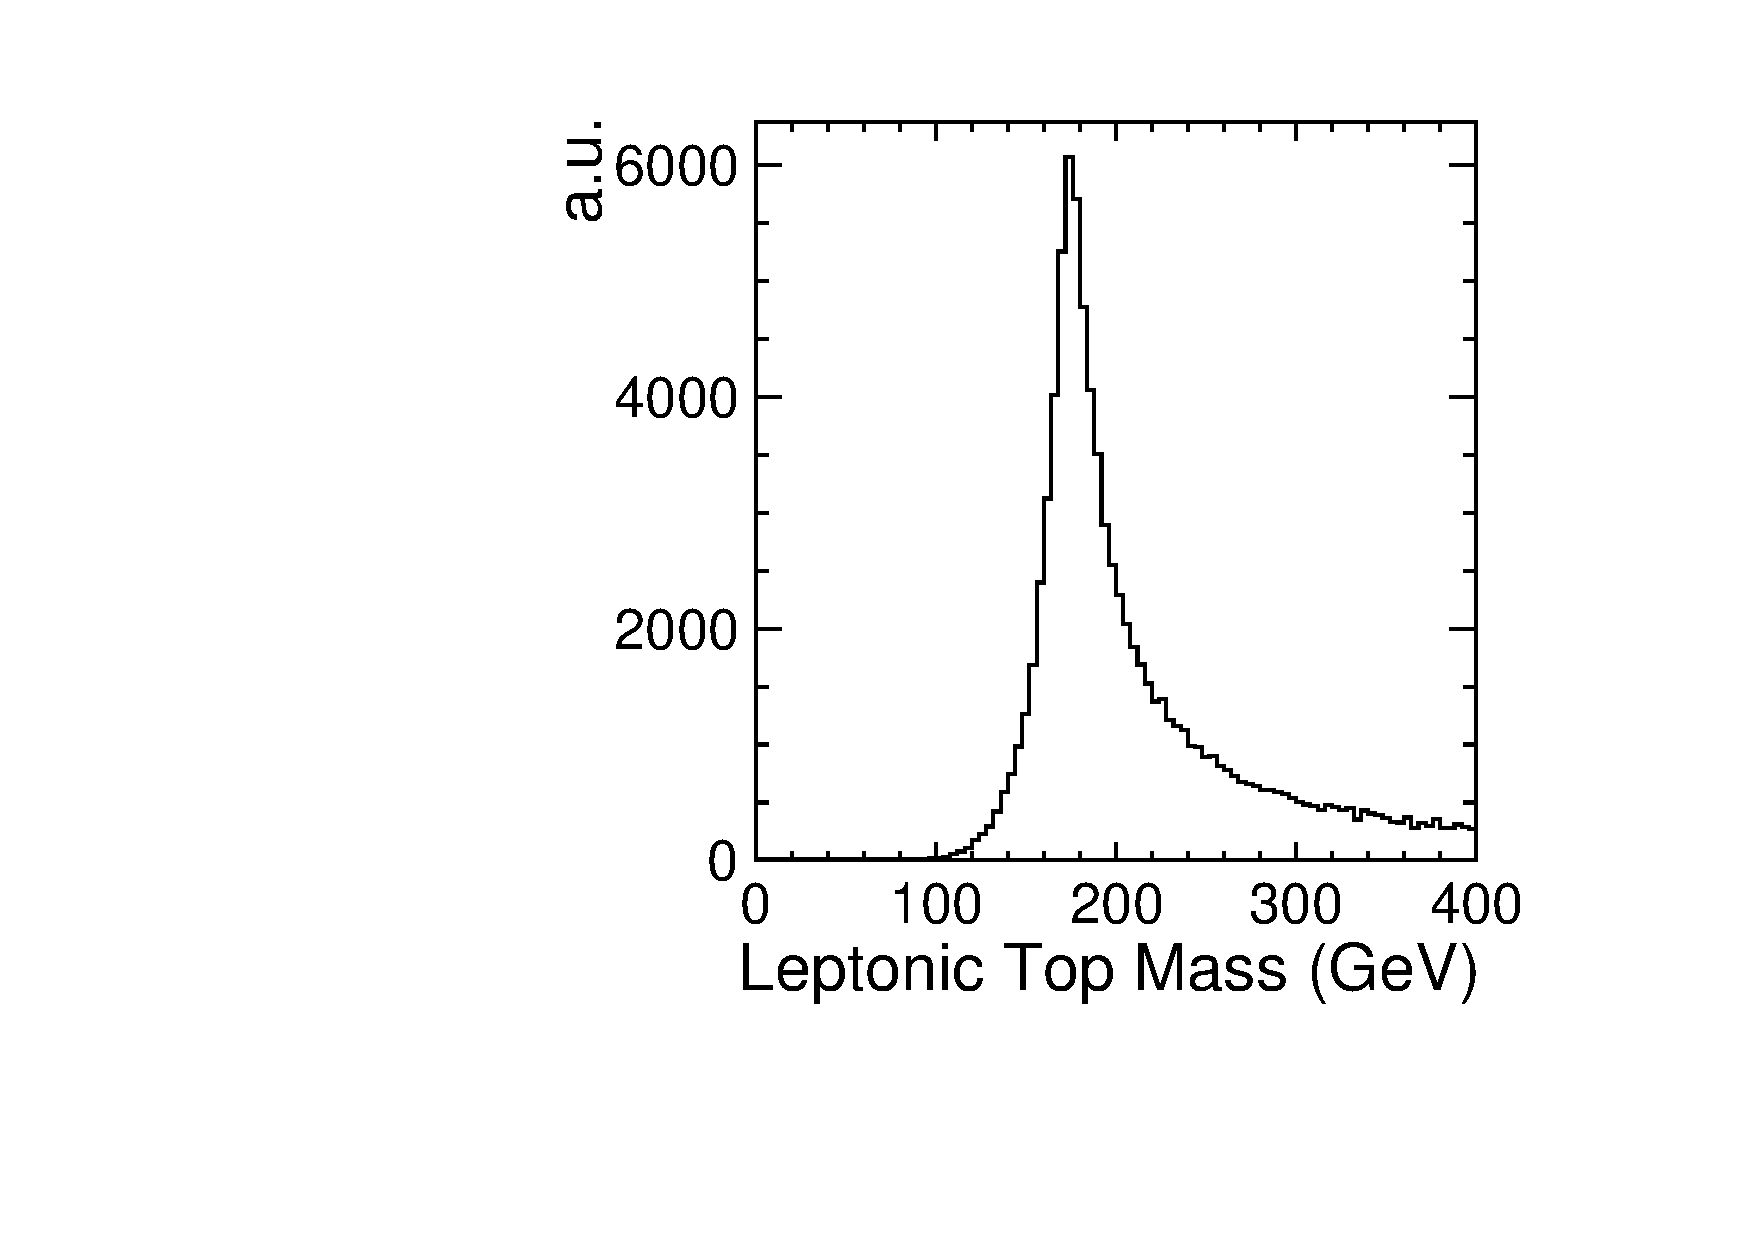
\includegraphics[width=0.6\textwidth]{TopAnalysis/figures/AnalTopMass.pdf}
  \caption[Mass of reconstructed leptonic top when using mass constraint method]{Mass of reconstructed top when using mass constraint method}
  \label{fig:TopMassFrommassMethod}
\end{figure}

The second method attempted is an adaptation of the first method that makes use of the high efficiency with which the lepton is reconstructed to improve the performance. This method was developed by a fellow member of \ac{CLIC}, Lars Rickard Str{\"o}m, based at \ac{CERN}. It starts in the same manner by assuming that all transverse missing momentum comes from the neutrino, however the missing longitudinal momentum is then divided beween the neutrino and photon. This is done by constraining the z component of the neutrino momentum by insisting the combination of the lepton and neutrino four momenta reproduces the W mass. Overall this acts to remove our incorrect assumption that the neutrino longitudinal momentum is negligible compared to the photons. The details of the calculations are as follows:

\begin{equation}
  p_W=p_l+p_\nu
\end{equation}
\begin{equation}
M_W^2=M_l^2 + 2(E_lE_\nu - \mathbf{p_l.p_\nu})
\end{equation}
\begin{equation}
0=-\frac{M_W^2-M_l^2}{2} + E_l.\sqrt{p^2_{\nu , x}+p^2_{\nu , y}+p^2_{\nu , z}} - (p_{\nu , x}p_{l , x}+p_{\nu , y}p_{l , y}+p_{\nu , z}p_{l , z})
\end{equation}
\begin{equation}
p_{\nu , z}=\frac{1}{2(p^2_{l , x}-E^2_{l})} (p_{l , z}(M_l^2-M_W^2)-2p_{l , z}(p_{l , x}p_{\nu , x}+p_{l , y}p_{\nu , y}) + X)
\end{equation}
Where,
\begin{equation}
  \label{eq:X}
  X=\sqrt{E_l^2((M_W^2-M_l^2 +2(p_{l , x}p_{\nu , x}+p_{l , y}p_{\nu , y}))^2 +4\epsilon_T^2(p^2_{l , z}-E_l^2) )}
\end{equation}
\begin{equation}
  \epsilon_T=\sqrt{p^2_{\nu , x}+p^2_{\nu , y}}
\end{equation}

In the event that X is imaginary, $\epsilon_T$ is scaled so that X=0. The key detail however, is that there is that there are two possible solutions for the neutrino momentum arrising from the quadratic form of \refeq{eq:X}. To decide the most suitable solution the W is combined with a fat jet (adding two more possible solutions, one for each fat jet) and the solution found to give an invariant mass closest to the top mass is chosen to be best. The resulting reconstructed leptonic top mass and s' reconstruction performance are shown in figures \ref{fig:MassConstraint} and \ref{fig:TopMassFrommassMethod}. The method does still have certain flaws that result in misreconstruction such as the assumption that all missing transverse momentum comes from the neutrinos and that the W mass is exactly 80.4 GeV with no associated width, however it clearly offers an improvement over the first method with a reasonable degree of agreement seen across the full s' range and a lower tendency to underestimate s'.

\subsubsection{Collinearity}

An alternative solution that was proposed was to use the collinearity (angular separation) of the $t\bar{t}$ pair as a way to measure s'. For collisions occurring at the nominal collision energy, the total momentum of the collison should be zero and so the two tops are produced back to back in the lab frame. If a photon is emitted before the electron positron collision occurs, the $t\bar{t}$ pair will have a none zero momentum and so will be boosted resulting in a reduced angular separation between the two tops. The scale of the boost (and thus the size of the angular separation) is proportional to the total momentum of the photon and so should be proportional to s'. Extraction of s' is performed by first using one sample to determine the exact relationship between the collinearity and the generator s'. This relationship is shown in \reffig{fig:Collinearity}. A calibration curve is then generated by fitting the profile of this with a second order polynomial. The performance is then evaluated by taking a second event sample and using the calibration curve to map back from the collinearity to a reconstructed s'. The resulting distribution for reconstruncted s' vs generator s' is shown in \reffig{fig:CollinearitySPrime}. Clearly this method is not as performant as the analytical method. One of the main reasons for this is that the collinearity should be measured between the two tops, however due to the neutrino not being reconstructed in the leptonic decay, one of the objects used for measuring the collinearity will be incomplete. This reduces the correlation between the collinearity and s'. Further, as s' decreases and the tops become less well separated, the chance of reconstruction failures occuring increases. Namely, the jet finding approach used will start to mix parts of each top when trying to construct two fat jets and so the objects the collinearity is calculated for will no longer correspond to the generator level tops (see \refsec{sec:jetassociation}.) This explains the very poor performance for the lowest s' events.

\begin{figure}
  \centering
  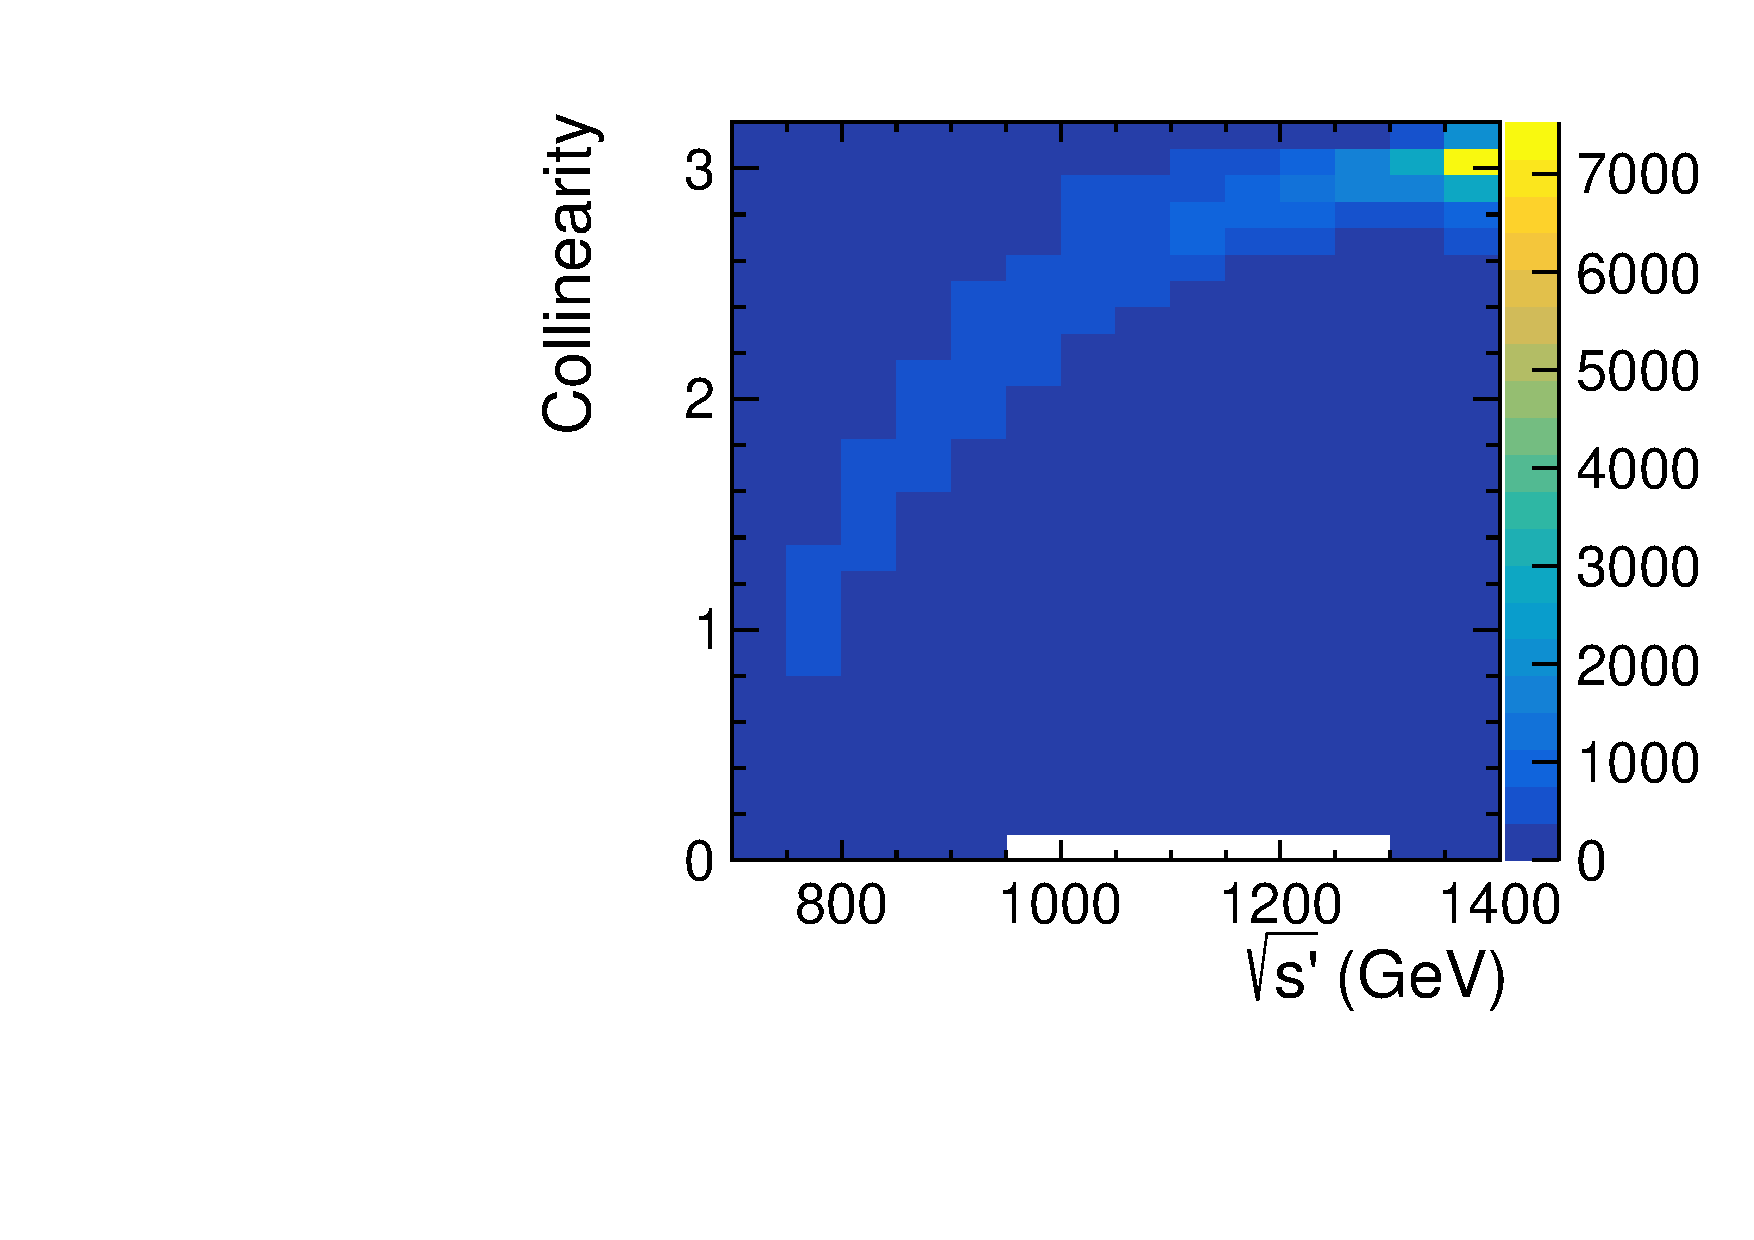
\includegraphics[width=0.6\textwidth]{TopAnalysis/figures/ColVsE.pdf}
  \caption[Collinearity of $t\bar{t}$ pair]{Collinearity of $t\bar{t}$ pair}
  \label{fig:Collinearity}
\end{figure}

\begin{figure}
  \centering
  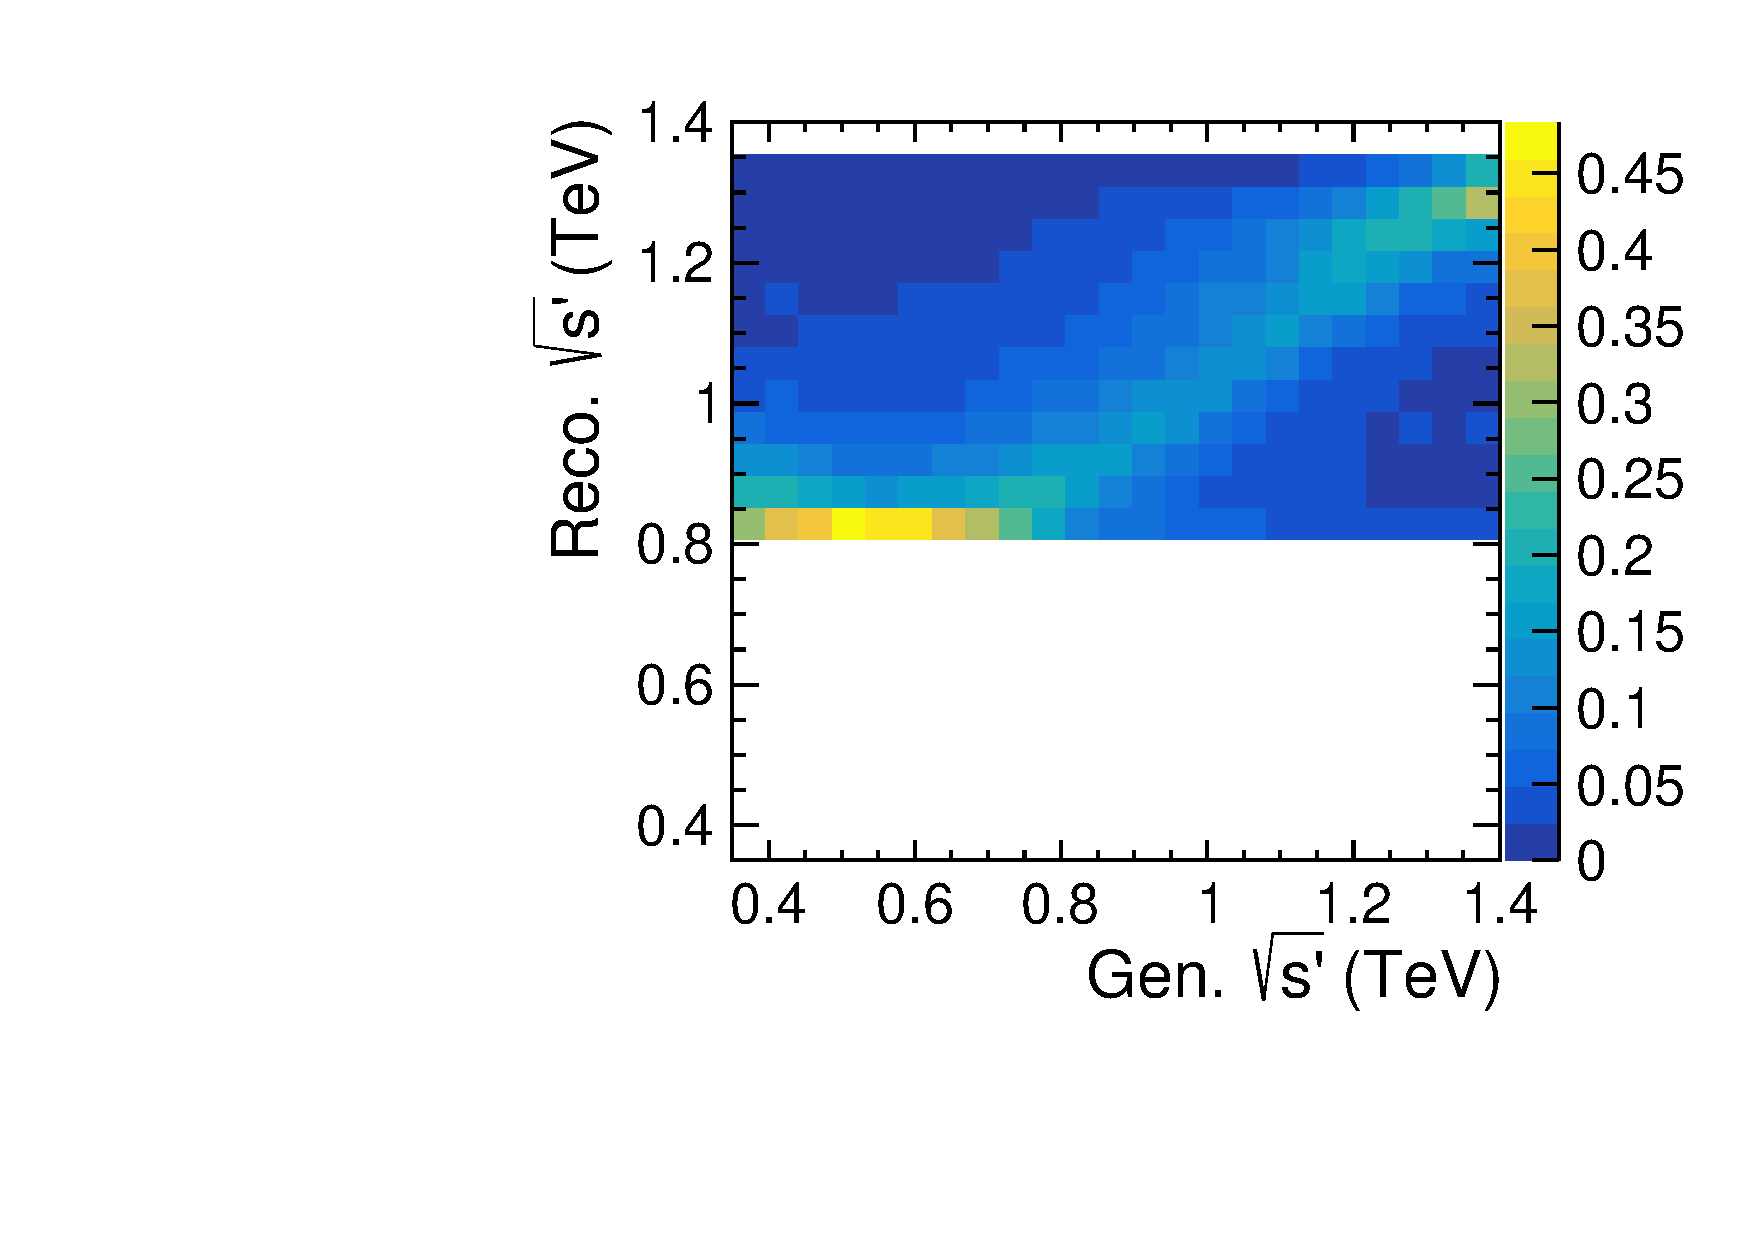
\includegraphics[width=0.6\textwidth]{TopAnalysis/figures/ColEVsTrueE.pdf}
  \caption[Reconstructed s' vs generator s' for collinearity method]{Reconstructed s' vs generator s' for collinearity method}
  \label{fig:CollinearitySPrime}
\end{figure}

\subsubsection{Kinematic Fitting}

The final approach considered was to use a kinematic fitter (MarlinKinFit v00-03\cite{List:88030}) to simultaneously fit the photon and and neutrino four momenta. The fit has four free parameters- the neutrinos three momentum and the photons z momentum (it is still assumed that photons have negligible transverse momentum) and has six contraints- the total four momentum of the system, the mass of the leptonically W and that the masses of the two tops are consistent. The fit is passed five fit objects- the isolated lepton, two fat jets, neutrino and photon.  The fit will try and find a solution that satisfies all the fit constraints by varying the four momenta of the fit objects. In the case of the physically obervable objects (the lepton and jets), the variation of the four momenta is limited according to the relevant detector resolutions:

\begin{align}
  \sigma_{E Had}&=35\%\sqrt{E}
  \\
  \sigma_{E EM}&=20\%\sqrt{E}
\\
  \sigma_{\theta/\phi}&=10\%
\end{align}

The photon power spectrum is also set within the fit by setting the parameter b in the following formula:

\begin{equation}
\frac{dN}{dp_z}\propto\frac{1}{p_z^{1-b}}
\end{equation}

A value of b=0.5 was found to give the best agreement for the reconstructed and generator s'. The resulting performance is shown in \reffig{fig:KinFit}. Overall the performance is similar to that of the analytic method with a good agreement seen between the reconstructed and generator s' across the full s' spectrum. It was decided that this method shall be used for s' determination for the rest of the analysis. While the analytical method is as performant, it is potentially less robust than the kinematic fitting due to the fact it uses a fixed top mass and is unable to scale the four momenta of the measured particles to compensate for detector resolutions.  For the rest of the analysis, the four momenta of all objects is taken to be those returned by the kinematic fit.

\begin{figure}
  \centering
  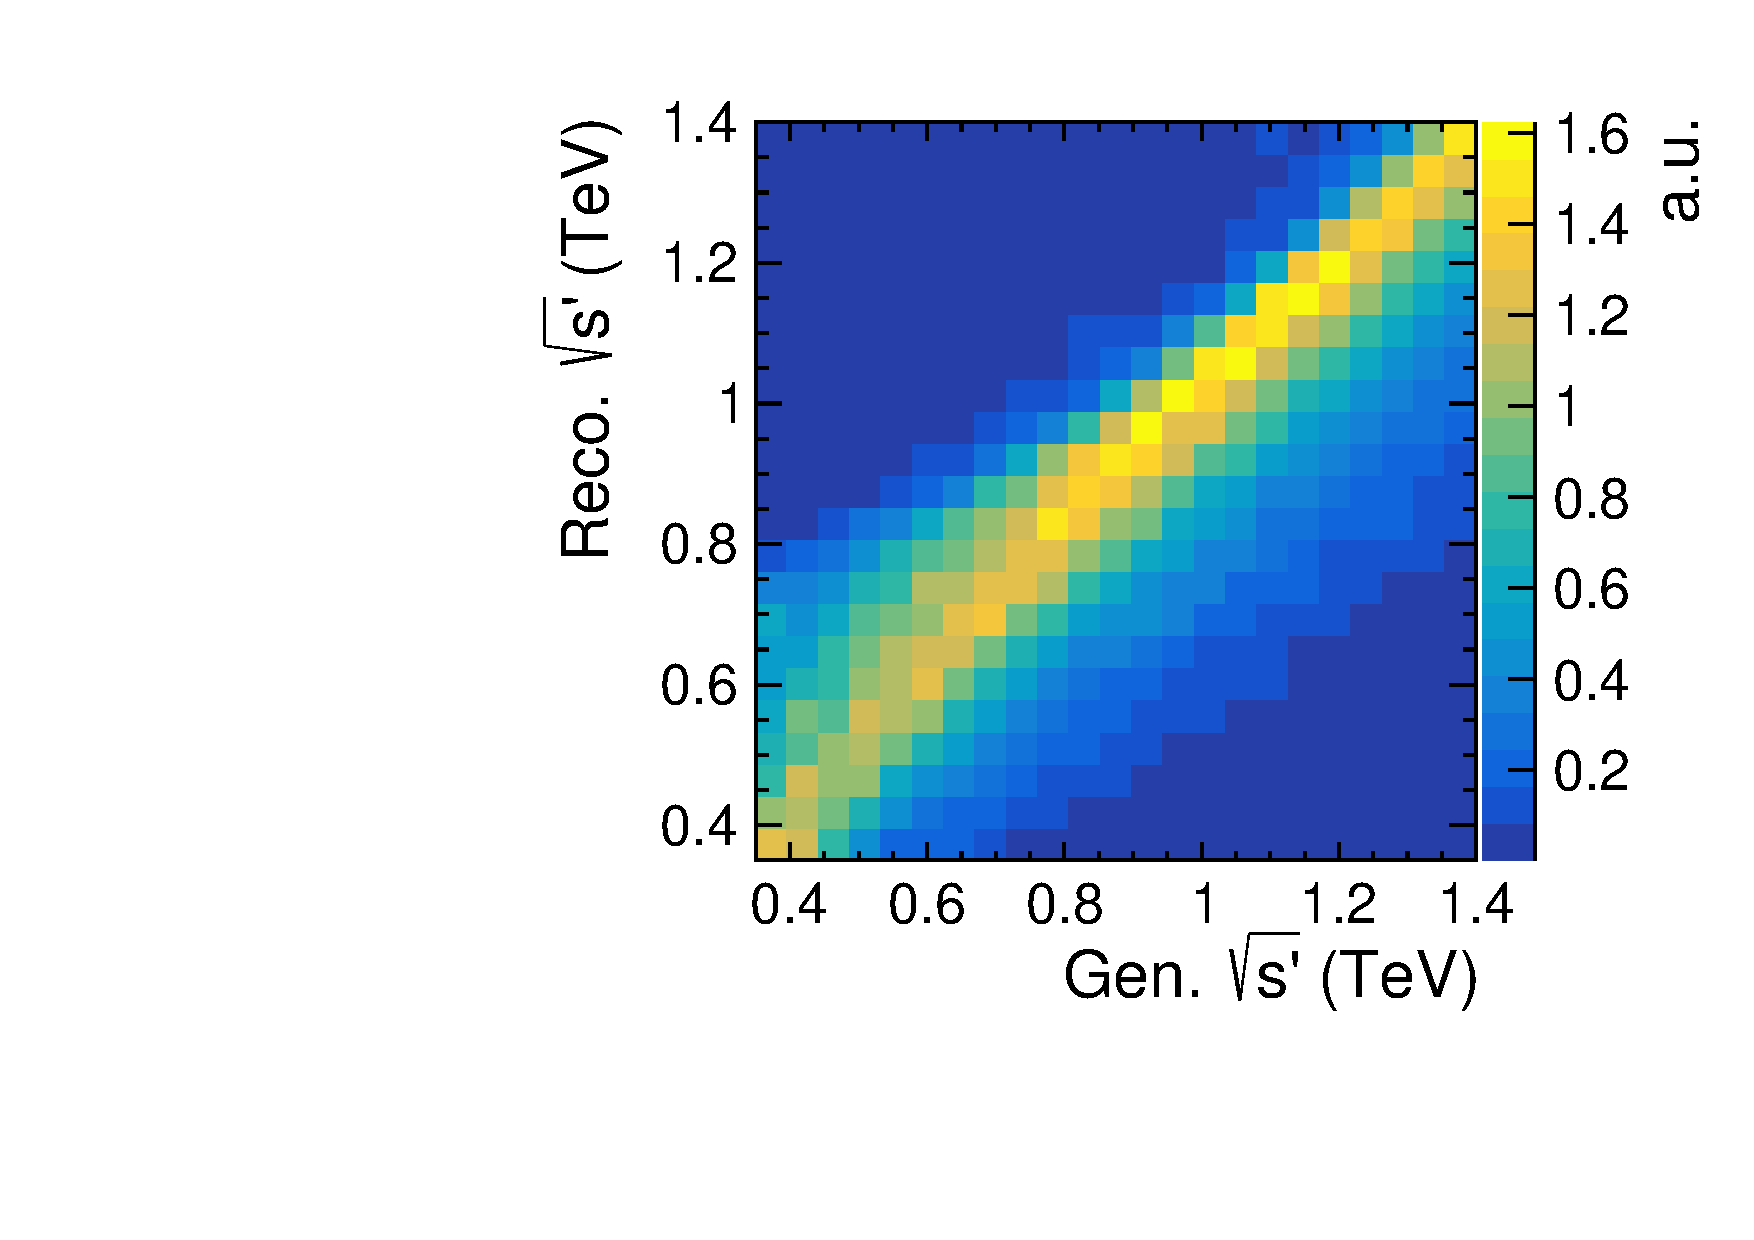
\includegraphics[width=0.6\textwidth]{TopAnalysis/figures/KinEVsTrueE.pdf}
  \caption[Reconstructed s' vs generator s' for kinematic fit  method]{Reconstructed s' vs generator s' for kinematic fit method}
  \label{fig:KinFit}
\end{figure}

\subsection{Flavour Tagging}
\label{Flavour Tagging}

\begin{figure}[t]
  \centering
  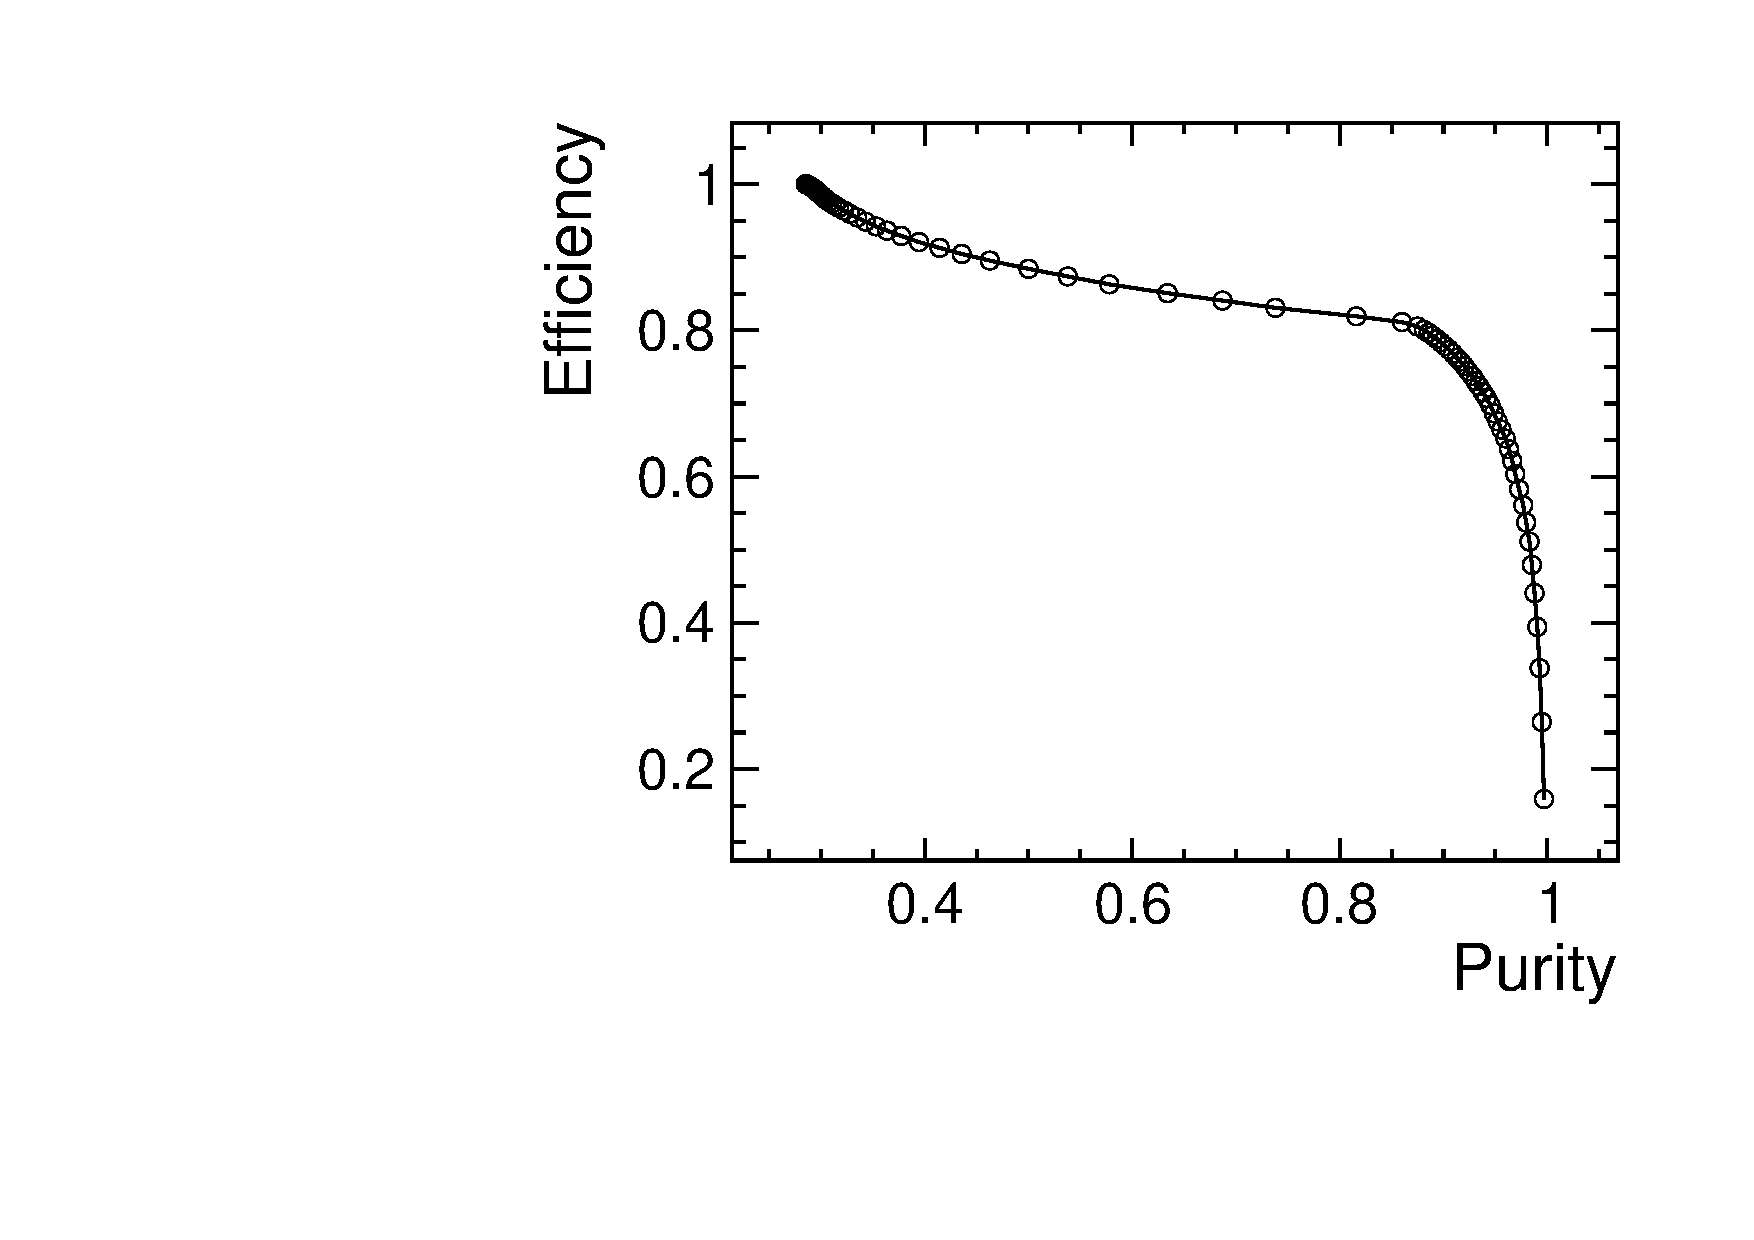
\includegraphics[width=0.78\textwidth,height=7cm,keepaspectratio]{HiggsAnalysis/figures/updatedpurityvsefficiency.pdf}
  \caption[B-Tagging Purity vs Efficiency]{Purity vs efficiency for identifying b-jets, obtained from a sample of Z$\rightarrow$ light, c and b quark events simulated at $\sqrt{s}=$1.4 TeV}
  \label{fig:Zbtagging}
\end{figure}

Flavour tagging was performed using LCFIPlus v00-05-02\cite{Suehara:2015ura}. LCFIPlus makes use of three BDTs dedicated to searching for u/d/s (light), b and c quarks respectively, to provide a b-tag and c-tag indicating the probability of a jet containing a b or c quark. As the signal process contains two b jets, only the results of the b-tag are considered here. The BDTs were trained using 50,000 $ee\rightarrow Z\nu\nu, Z\rightarrow qq$ events each. The base performance of the BDTs was assessed using a further 150,000 $ee\rightarrow Z\nu\nu, Z\rightarrow qq$ events containing an even mixture of bb, cc and light quarks to measure the efficiency and purity that could be obtained. The results of this test (shown in \ref{fig:Zbtagging}) indicate that in the case of Z$\rightarrow$qq events high efficiencies and puritys of \~85\% can be acieved simultaneously. Before we apply the flavour tagging to our analysis we first recluster our events into four jets to try and capture the bjets separately from the light quark jets. This is done within the LCFIPlus package which uses the Durham algorithm by default. Ideally the BDTs would also be retrained using top events rather than Z, however due to limited sample sizes this was not a realistic option. The performance of the btagging for semileptonic top events was evaluated by comparing the highest and second highest b-tags assigned to any of the four jets in signal events to those in backgrounds. The results of this comparison are seen in figure \ref{fig:btagging}. It is clear that the btagging is consistantly successful in finding the first b jet, but is less reliable for finding a second b jet. This is expected due to the toplogy of the event. The b jet produced by the leptonically decaying top should be well isolated from everything but the lepton which is identified and removed with high efficiency whereas the bjet from hadronically decaying top will be close to two other jets meaning the jet finder is less likely to accurately associate the PFOs in that region to the correct initial quark. As a result the b jet from the leptonic side should be consistently reconstructed and tagged whereas the the b jet on the hadronic side will be less consistent as the efficiency for reconstructing the jet correctly is much lower. Despite the poorer perfomrnace of the second highest b-tag, both variables provide clear potential as discriminating variables for removing background. 


\begin{figure}
  \centering
  \begin{subfigure}{.5\textwidth}
    \centering
    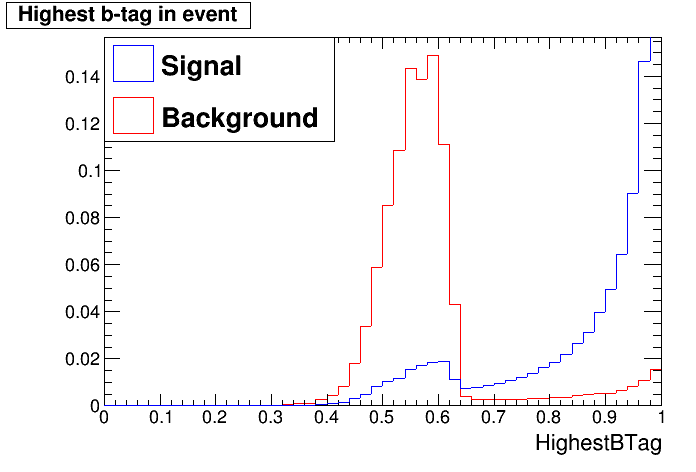
\includegraphics[width=0.9\textwidth]{TopAnalysis/figures/HighestBTag_SigVsBkg.png}
    \caption[Highest b-tag in event]{Highest b-tag in event}
  \end{subfigure}%
  \begin{subfigure}{.5\textwidth}
    \centering
    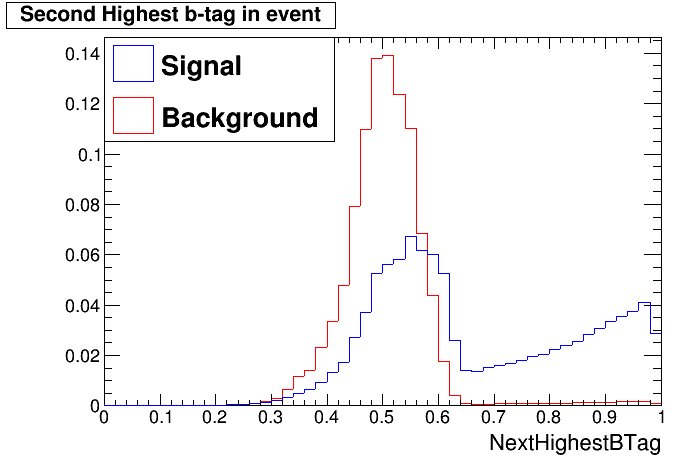
\includegraphics[width=0.9\textwidth]{TopAnalysis/figures/NextHighestBTag_SigVsBkg.png}
    \caption[Second Highest b-tag event in event]{Second Highest b-tag in event}
  \end{subfigure}
  \caption[B-Tagging performance]{B-Tagging performance}
  \label{fig:btagging}
\end{figure}


\section{Methods For Calculating AFB}
\label{Calculating AFB}

Measuring AFB from theta distributions vs counting- benefit that theta fit isn't effected by acceptance cutoff
Show relative precision for Afb for MC only for different methods


\section{Event Selection}
\label{Event Selection}


Split into three regions- low and high energy due to different topology from s'

Using bdt based selection to maximise performance


\subsection{Preselection}
Preselection cuts

\subsection{Quality Cuts}
\label{Quality Cuts}

\subsection{BDT Selection}
BDT variables

Large table showing efficiency of all cuts on all samples and the final expected number of events for full luminosity

Overall signal efficiency/purity/significance

\section{Extraction of AFB and xsec}
Differential version of at least one of the plots- probably just signal before selection and then signal+background after selection with background subtraction.
Explain that most precise point will be for s' >1200 as there is the cleanest signal- highly boosted jets.
Suggest that lower s' results could benefit from a different reconstruction approach based on a resolved 4 jet analysis- probably deserves its own dedicated study though we can do if we have time. Would also likely benefit from having different variables used for the low s' BDT.

\section{Systematics}

\section{Improvements}

\section{Conclusions}

We measured the Afb to x precision....
